\documentclass[twoside,english, a4paper, 12pt]{uiofysmaster}
% \usepackage{biblatex}
\usepackage{todonotes}

\author{Anders Hafreager}
\title{\uppercase{Flow in nanoporous media}}
\date{October 2013}

\usepackage{listings}
\usepackage{xcolor}
\usepackage{amsmath}
\usepackage{amssymb}
% \usepackage[hidelinks]{hyperref}
\usepackage{hyperref}
\usepackage[T1]{fontenc}
\usepackage{bbold}
\usepackage{simplewick}
\usepackage[squaren]{SIunits}
\usepackage{sidecap}
\usepackage[titletoc]{appendix}

\definecolor{grey}{rgb}{0.98,0.98,0.98}
\definecolor{codeRed}{rgb}{0.5, 0.027, 0.02}

% Code parameters
\lstset{language=c++}
\lstset{basicstyle=\small}
\lstset{backgroundcolor=\color{white}}
\lstset{frame=single}
\lstset{stringstyle=\ttfamily}
\lstset{keywordstyle=\color{codeRed}\bfseries}
\lstset{commentstyle=\itshape\color{gray}}
\lstset{showspaces=false}
\lstset{showstringspaces=false}
\lstset{showtabs=false}
\lstset{breaklines}

\setlength{\parskip}{11pt}
\setlength{\parindent}{0mm}

\lstset{
language=Python,
basicstyle=\footnotesize
frame=single,
backgroundcolor=\color{grey}
}

\lstset{
language=Matlab,
basicstyle=\footnotesize,
frame=single,
backgroundcolor=\color{grey}
}

\lstset{
language=C++,
backgroundcolor=\color{grey}
}

\lstdefinelanguage{GLSL}
{
sensitive=true,
morekeywords=[1]{
attribute, const, uniform, varying,
layout, centroid, flat, smooth,
noperspective, break, continue, do,
for, while, switch, case, default, if,
else, in, out, inout, float, int, void,
bool, true, false, invariant, discard,
return, mat2, mat3, mat4, mat2x2, mat2x3,
mat2x4, mat3x2, mat3x3, mat3x4, mat4x2,
mat4x3, mat4x4, vec2, vec3, vec4, ivec2,
ivec3, ivec4, bvec2, bvec3, bvec4, uint,
uvec2, uvec3, uvec4, lowp, mediump, highp,
precision, sampler1D, sampler2D, sampler3D,
samplerCube, sampler1DShadow,
sampler2DShadow, samplerCubeShadow,
sampler1DArray, sampler2DArray,
sampler1DArrayShadow, sampler2DArrayShadow,
isampler1D, isampler2D, isampler3D,
isamplerCube, isampler1DArray,
isampler2DArray, usampler1D, usampler2D,
usampler3D, usamplerCube, usampler1DArray,
usampler2DArray, sampler2DRect,
sampler2DRectShadow, isampler2DRect,
usampler2DRect, samplerBuffer,
isamplerBuffer, usamplerBuffer, sampler2DMS,
isampler2DMS, usampler2DMS,
sampler2DMSArray, isampler2DMSArray,
usampler2DMSArray, struct},
morekeywords=[2]{
radians,degrees,sin,cos,tan,asin,acos,atan,
atan,sinh,cosh,tanh,asinh,acosh,atanh,pow,
exp,log,exp2,log2,sqrt,inversesqrt,abs,sign,
floor,trunc,round,roundEven,ceil,fract,mod,modf,
min,max,clamp,mix,step,smoothstep,isnan,isinf,
floatBitsToInt,floatBitsToUint,intBitsToFloat,
uintBitsToFloat,length,distance,dot,cross,
normalize,faceforward,reflect,refract,
matrixCompMult,outerProduct,transpose,
determinant,inverse,lessThan,lessThanEqual,
greaterThan,greaterThanEqual,equal,notEqual,
any,all,not,textureSize,texture,textureProj,
textureLod,textureOffset,texelFetch,
texelFetchOffset,textureProjOffset,
textureLodOffset,textureProjLod,
textureProjLodOffset,textureGrad,
textureGradOffset,textureProjGrad,
textureProjGradOffset,texture1D,texture1DProj,
texture1DProjLod,texture2D,texture2DProj,
texture2DLod,texture2DProjLod,texture3D,
texture3DProj,texture3DLod,texture3DProjLod,
textureCube,textureCubeLod,shadow1D,shadow2D,
shadow1DProj,shadow2DProj,shadow1DLod,
shadow2DLod,shadow1DProjLod,shadow2DProjLod,
dFdx,dFdy,fwidth,noise1,noise2,noise3,noise4,
EmitVertex,EndPrimitive},
morekeywords=[3]{
gl_VertexID,gl_InstanceID,gl_Position,
gl_PointSize,gl_ClipDistance,gl_PerVertex,
gl_Layer,gl_ClipVertex,gl_FragCoord,
gl_FrontFacing,gl_ClipDistance,gl_FragColor,
gl_FragData,gl_MaxDrawBuffers,gl_FragDepth,
gl_PointCoord,gl_PrimitiveID,
gl_MaxVertexAttribs,gl_MaxVertexUniformComponents,
gl_MaxVaryingFloats,gl_MaxVaryingComponents,
gl_MaxVertexOutputComponents,
gl_MaxGeometryInputComponents,
gl_MaxGeometryOutputComponents,
gl_MaxFragmentInputComponents,
gl_MaxVertexTextureImageUnits,
gl_MaxCombinedTextureImageUnits,
gl_MaxTextureImageUnits,
gl_MaxFragmentUniformComponents,
gl_MaxDrawBuffers,gl_MaxClipDistances,
gl_MaxGeometryTextureImageUnits,
gl_MaxGeometryOutputVertices,
gl_MaxGeometryOutputVertices,
gl_MaxGeometryTotalOutputComponents,
gl_MaxGeometryUniformComponents,
gl_MaxGeometryVaryingComponents,gl_DepthRange},
morecomment=[l]{//},
morecomment=[s]{/*}{*/},
morecomment=[l][keywordstyle4]{\#},
}

% ------------------------------------------------- COLOR BOX
                                                                

\renewcommand{\vec}{\mathbf}
\newcommand{\mat}{\mathbf}
\newcommand{\F}{\mathbf{F}}
\newcommand{\E}{\mathbf{E}}
\newcommand{\B}{\mathbf{B}}
\newcommand{\J}{\mathbf{J}}
\newcommand{\R}{\mathbf{R}}
\newcommand{\avec}{\mathbf{a}}
\newcommand{\rvec}{\mathbf{r}}
\newcommand{\vvec}{\mathbf{v}}
\newcommand{\xvec}{\mathbf{x}}
\newcommand{\diverg}{\nabla \cdot}
\newcommand{\curl}{\nabla \times}
\newcommand{\laplace}{\nabla^2}
\newcommand{\definition}{\emph}
\newcommand{\dpart}[2]{\frac{\partial #1}{\partial #2}}
\newcommand{\dd}[2]{\frac{\mathrm{d}#1}{\mathrm{d}#2}}
\newcommand{\unit}[1]{\hat {\vec{#1}}}

% Quantum stuff
\newcommand{\infint}{\int_{-\infty}^{\infty}}

% Equations
\newcommand{\bea}{\begin{eqnarray*}}
\newcommand{\eea}{\end{eqnarray*}}
\newcommand{\beq}{\begin{equation}}
\newcommand{\eeq}{\end{equation}}

\usepackage{mathrsfs}

% \usepackage{autocite}
\usepackage[]{biblatex}
\bibliography{Bibliography/master.bib}

\begin{document}

\maketitle
\clearpage

\begin{abstract}
This is an abstract text.
\end{abstract}
\begin{dedication}
  To someone
  \\\vspace{12pt}
  This is a dedication to my cat.
\end{dedication}
\begin{acknowledgements}
  I acknowledge my acknowledgements.
\end{acknowledgements}

\tableofcontents
\clearpage
\listoffigures
\clearpage
\listoftables

\begin{chapter}{Introduction}
  \section{Introduction}


\subsection{Motivation}


\subsection{The structure of this thesis}


\section{My contribution}

\end{chapter}

\begin{chapter}{Theory of fluids}
  Most people have an intuition about what a substance is. A substance is just \textit{something}, like water, wood, butter or glass. A metal is a substance. The blood in your body is a substance. All of these are made up of atoms that form molecules in ways giving them very different properties. We know that a substance can exist in different phases, for example plasma, solid, liquid and gas \cite{ravndal2008statmech}, in which the same substance can behave very differently. Liquids and gases are often called fluids because they share the property that they do not have a fixed shape and is often easily deformed. In this chapter we will briefly go through the history of fluids, and discuss how the theory of fluids was developed from the discoveries by the ancient greeks to modern fluid mechanics. \\
We start this chapter with section \ref{sec:theory_of_fluids_greece} by quoting some of the great minds from Greece who were the first to describe fluids in a scientific way, before we discuss the Euler equations and Navier-Stokes equations in section \ref{sec:theory_of_fluids_euler_navier}. These sets of equations assume that the fluid can be described as a continuum, which turns out not to be true for what is called \textit{microflows}. The discussion about macroflows and microflows leads up to what is called the breakdown of continuum which is addressed in section \ref{sec:continuum_breakdown}. One very important effect is the slip velocity which leads to discrepancies from the standard continuum solver approach. This is discussed in section \ref{sec:slip_length}, before we in section \ref{sec:knudsen_number} introduce the Knudsen number which allows us to define different flow regimes in which we can categorize the validity of different fluid flow models.\\
We then define what a nanoporous media is before we in section \ref{sec:darcy_law} discuss permeability and Darcy's law and that we need to apply corrections to the permeability because of the effects of slip velocity.
\section{The beginning in Greece}
\label{sec:theory_of_fluids_greece}
The first scientific descriptions of fluid mechanics dates back to Aristotle (384-322 B.C.) when he identified the continuum and dynamic drag in fluids \cite{anderson1998history}. He wrote
\begin{aquote}{Aristotle by Lysippus}
The continuous may be defined as that which is divisible into parts which are themselves divisible to infinity, as a body which is divisible in all ways. Magnitude divisible in one direction is a line, in three directions a body. And magnitudes which are divisible in this fashion are continuous. 
\end{aquote}
The idea of continuum is fundamental in most fluid mechanics theories and is a rather abstract concept that makes the mathematics work out beautifully. At the time of Aristotle, the mathematical framework was not yet established, so it was an impressive contribution to the field. The more intuitive drag force was described as
\begin{aquote}{Aristotle by Lysippus}
It is impossible to say why a body that has been set in motion in a vacuum should ever come to rest. Why, indeed, should it come to rest at one place rather than another. As a consequence, it will either necessarily stay at rest, or if in motion, will move indefinitely unless some obstacle comes into collision with it.
\end{aquote}
For fluids in movement, the obstacle is the thing creating the drag force preventing the fluid to move freely. About a hundred years later, Archimedes (287-212 B.C.) published \textit{On Floating Bodies} where he discussed what is now known as \textit{Archimedes' principle} that states
\begin{aquote}{Archimedes of Syracuse}
Any object, wholly or partially immersed in a fluid, is buoyed up by a force equal to the weight of the fluid displaced by the object.
\end{aquote}
Even today, more than 2000 years later, every high school student taking a physics course learn about Archimedes' principle. It is a simple and intuitive, yet remarkably powerful, statement that can easily be derived using Newtonian mechanics. 

\section{The Euler equations and the Navier-Stokes equations}
\label{sec:theory_of_fluids_euler_navier}
With the concept of continuum, we think that each point in space has well defined physical properties like temperature, density and momentum. In 1757, Euler published what's called the \textit{Euler equations} by applying conservation of mass, momentum and energy to a small volume element $\dm V$. It is a set of differential equations describing how the fluid velocity field changes in time and space. The conservation laws can be written as
\begin{align}
	\dpart{\rho_m}{t} + \nabla\cdot (\rho_m\vec u) &= 0 \qquad \text{mass}\\
	\dpart{\rho_m \vec u}{t} + \nabla \cdot (\vec u \otimes (\rho_m\vec u)) + \nabla P &= 0\qquad \text{momentum}\\
	\dpart{E}{t} + \nabla\cdot (\vec u(E + p)) &= 0\qquad \text{energy},
\end{align}
where $\rho_m$ is the mass density, $\vec u(\vec x, t)$ is the velocity field, $E$ is the total energy per unit volume, $\otimes$ is the tensor product and $P(\vec x, t)$ is the pressure field. These can be combined to one vector equation, but the idea of conservation laws are more clear when they are separated. In the original paper, Euler only derived the first two equations, but the full set is usually referred to as the Euler equations. They describe the motion of fluids with negligible viscosity which is a decent approximation for many fluids.\\
About 80 years later, in the 1840s, Sir George Stokes published the Navier-Stokes equations (NSE) which can be seen as an extension of the Euler equations where effects caused by the viscosity of the fluid are included \cite{batchelor2000introduction}. The Navier-Stokes equations for an incompressible fluid can be written as one vector equation
\begin{align}
	\label{eq:nse_incompressible}
	\rho_m \frac{D\vec u}{Dt} = \rho_m \vec F - \nabla p + \mu\nabla^2\vec u,
\end{align}
where $\vec F$ is an external force (i.e. gravity or an electrostatic field), $\mu$ is the viscosity and $D/Dt$ is the material derivative defined as
\begin{align}
	\frac{D}{Dt} = \dpart{}{t} + \vec u\cdot \nabla.
\end{align}
These are also a set of coupled non-linear differential equations that can be seen as one vector differential equation. It has quite a few interesting analytically solvable solutions, but for most real systems, the geometry confining the fluid is so complex that it is usually solved on computers. The equation above is valid for incompressible fluids where the mass-conservation equation is written as (constant density)
\begin{align}
	\nabla\cdot \vec u = 0,
\end{align}
which is a good approximation for many liquids. However, most gases are compressible, and the more general NSE including theses effects is given as
\begin{align}
	\rho_m \frac{D\vec u}{ Dt} = \rho_m \vec F - \nabla p + \mu\nabla^2\vec u + \mu\nabla(\nabla\cdot \vec u),
\end{align}
where we notice the extra term compared to equation \eqref{eq:nse_incompressible}. When solving the NSE, one has to provide boundary conditions to get a unique solution for the system. Usually, one applies no-slip boundary conditions, i.e. that the fluid velocity is zero at the container walls. In section \ref{sec:slip_length} we discuss the effects of slip velocity and how this affects the flow properties of the fluid. 

\section{Macroflows and microflows}
\label{sec:theory_of_fluids_microflows}
When we solve the equations governing our fluid flow, we add boundary conditions defining the geometry of our system. In the 1990s H. Bau and J. Zemel (University of Pennsylvania) performed experiments on microchannel flow in which they found clear deviations from what was expected from the theory\cite{karniadakis2005microflows}. It is useful to introduce the terms \textit{microflows} for flow in geometries where the distance between the channel walls is of micrometer size and \textit{macroflows} for larger systems (milimeter and above). Flow at microscales differ from macroscales because of effects that can be classified into four groups
\begin{itemize}
\item noncontinuum effects,
\item surface-dominated effects,
\item low Reynolds number effects, and
\item multiscale and multiphysics effects.
\end{itemize}
In this thesis, we focus on the noncontinuum effects which are briefly discussed in section \ref{sec:continuum_breakdown}, and the surface-dominated effects as the slip condition described in section \ref{sec:slip_length}. See \cite{karniadakis2005microflows} for details about the effects of low Reynolds number, multiscale and multiphysics. 

\section{The breakdown of continuum}
\label{sec:continuum_breakdown}
A fundamental assumption in the derivation of the NSE is that the space is continuous. We know that in reality, the mass of the fluid is concentrated in the very center of the atoms, but we often assume that the mass is uniformly distributed in the volume element of which the conservations laws are applied on. This is known as the \textit{continuum hypothesis} and is invalid when the \textit{mean free path} $\lambda$, the average distance a particle moves between collisions, becomes large compared to some characteristic length $L$ in the system, i.e. the diameter of a channel\cite{karniadakis2005microflows}. This property is quantified through the \textit{Knudsen number}
\begin{align}
	\text{Kn} = \frac{\lambda}{L}.
\end{align}
From the kinetic theory we can calculate the mean free path (which is done in section \ref{sec:mean_free_path_calculation})
\begin{align}
	\lambda = \frac{m}{\sqrt 2 \pi d \rho_n} = \frac{k_B T}{\sqrt 2 \pi d^2 P},
\end{align}
where $\rho_n$ is the number density and $m$ and $d$ are the mass and diameter of the particles. By inserting the ideal gas law $P = \rho_n k_BT$, we can eliminate the density and use the pressure $P$ together with the temperature $T$ instead. Here $k_B$ is of course Boltzmann's constant. For Knudsen numbers smaller than $10^{-2}$, the continuum hypthosis is valid and we can apply the Navier-Stokes equations\cite{karniadakis2005microflows}. The Knudsen number is so important that it deserves its own section.

\section{Slip velocity}
\label{sec:slip_length}
The Navier-Stokes equations need boundary conditions of the velocity field defining the geometry of which the fluid is confined in. As mentioned earlier, the simplest boundary condition is the no-slip condition where
\begin{align}
	\vec u(\vec r; t) = 0 \qquad \vec r \in \partial\Omega
\end{align}
where $\partial\Omega$ defines the boundary domain. The history of the no-slip condition is studied by Day, based on the work of Stokes in the 19th century. Stokes compared theoretical results to experiments for pendulums of different kinds and concluded that\cite{day1990no}
\begin{aquote}{Stokes, 1901}
	I shall assume, therefore, as the conditions to be satisfied at the boundaries of the fluid, that the velocity of a fluid particle shall be the same, both in magnitude and direction, as that of the solid particle with which it is in contact. The agreement of the results thus obtained with observation will presently appear to be highly satisfactory.
\end{aquote}
In Day's detailed study of the no-slip condition, he says
\begin{aquote}{Day, 1990}
	Looking back, it appears that the acceptance of a more general no-slip condition was prolonged because of experimental shortcomings, not because of a lack of the \'appropriate\' theoretical solutions to fluid flow problems.
\end{aquote}
In other words, the theoretical framework that existed already in the time of Stokes were complete enough to include both slip and no-slip solutions. In fact, Maxwell predicted slip velocity in a paper already in 1867\cite{maxwell1879stresses}, but the experiments the next 50 years seemed to more or less confirm the no-slip condition. \todo{Discuss the later experiments showing discrepancies} Klinkenberg also has a nice argument that supports the slip velocity
\begin{aquote}{L.J. Klinkenberg, 1941}
Consider a layer adjacent to the wall which is thinner than the mean free path $\lambda$ of the gas molecules, so that practically a molecule does not collide with other molecules present in this layer. At a given moment half of the gas molecules in this layer will have a component of velocity moving towards the wall; the other half in the opposite direction. The molecules moving towards the wall have had their last collision somewhere in the flowing mass, and, therefore, will have an average velocity component in the direction of flow different from zero. A part of this average velocity component will be lost in colliding with the wall. Even if the molecules lose it entirely, then still the average velocity component in the direction of flow of all the molecules contained in the layer will amount to half of the average velocity component of the molecules moving towards the wall. The gas in the layer, therefore, will have a finite rate of flow.
\end{aquote}
It is convenient to introduce the concept of \textit{slip length} $l_s$ to be able to quantify the slip velocity. Slip length is defined as the distance into the wall we would have to extrapolate a velocity profile for it to reach zero value, see figure \ref{fig:slip_length}.
\begin{figure}[h]
\begin{center}
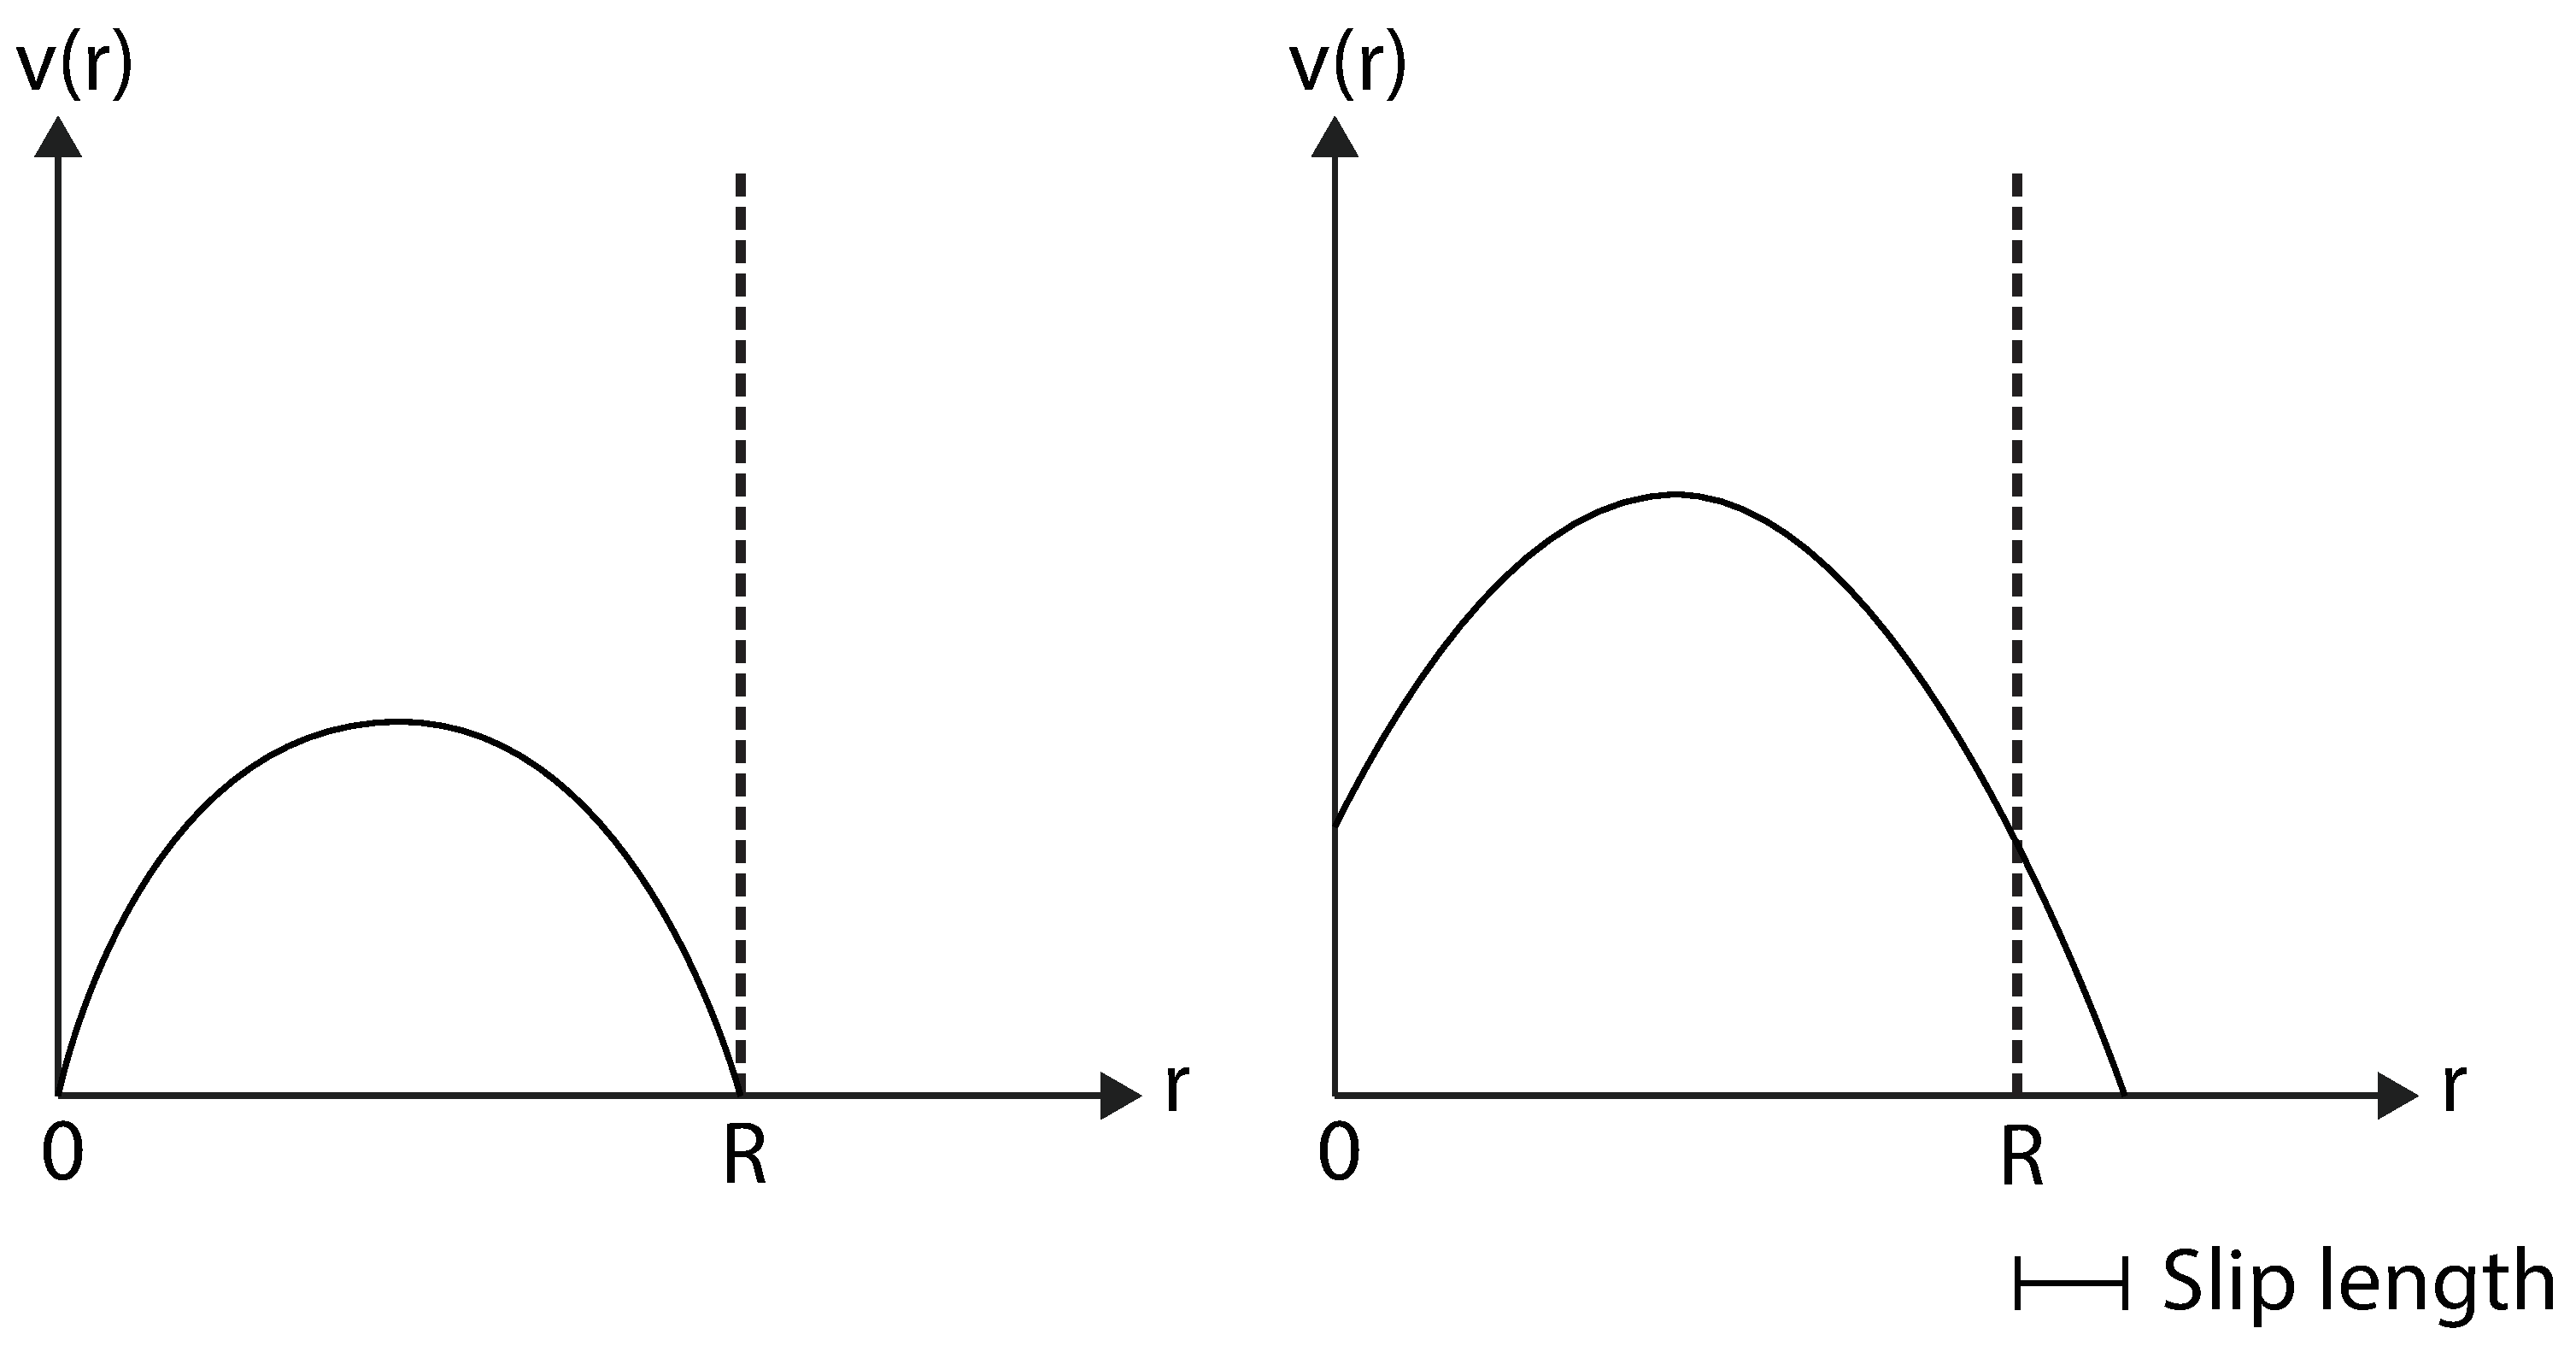
\includegraphics[width=\textwidth, trim=0cm 0cm 0cm 0cm, clip]{DSMC/figures/slip_length.eps}
\end{center}
\caption{Slip length is the distance into the wall we would have to extrapolate a velocity profile for it to reach zero value. We have the no-slip condition on the left, where the slip length is zero whereas we have a non-zero slip length on the right.}
\label{fig:slip_length}
\end{figure}
Maxwell theory predicts the following relation between the slip length and the mean free path
\begin{align}
	\label{eq:noslip_sliplength}
	l_s = \alpha \lambda,
\end{align}
where $\alpha\approx 1.15$ is the slip coefficient \cite{morris1992slip}. The effects of slip velocity become more apparent when the channel diameter is of the same order as the mean free path. By introducing the dimensionless slip length
\begin{align}
	l_s^* = \frac{l_s}{ L} = \alpha \frac{\lambda }{ L} = \alpha \text{Kn},
\end{align}
we see that the ratio of the slip length to the channel diameter is proportional to the Knudsen number. The actual slip velocity (the average velocity of the molecules right next to the wall) can be written as
\begin{align}
	\label{eq:linear_slip_velocity}
	v_{\text{wall}} = \alpha\lambda\frac{\dm v}{\dm n},
\end{align}
where $n$ is the direction normal on the wall\cite{klinkenberg1941permeability}. We call this a \textit{first order} slip model since it is contains only the first derivative of the velocity. Higher order models exists and give corrections that are important in nanoporous media (which is defined in section \ref{sec:nanoporous_media}) where the channels that contribute to flow are of nanometer scale.

\section{Knudsen number}
\label{sec:knudsen_number}
To get an idea of the length scales where the Knudsen number is about unity, the mean free path for helium at $T=$\unit{273}{\kelvin} and $P=1$ atm is\cite{lillestol2001generell} 
\begin{align}
	\label{eq:helium_mfp}
	\lambda_{\text{He}} = \unit{0.17}{\micro\meter} = \unit{170}{\nano\meter}.
\end{align}
This means that for systems where the channels have diameter of a few hundred nanometers, the Knudsen number is around unity, and the continuum hypothesis is invalid. 

\section{Atomic models}
\label{sec:theory_of_fluids_atomic_models}
For systems where the continuum hypothesis is invalid, we need other models describing the behaviour of the particles in our system. The first idea that might pop our minds might be to study the system at the atomic level. The physical set of rules that are controlling the atoms is of course quantum mechanics. The equations of motion and hence the dynamics of an atomic system can in principle be calculated directly from quantum mechanics by solving Schr\"{o}dinger's equation with perturbation theory. Since this requires calculating the wave function of every atom with complex atomic interactions, the size of the system needs to be very small with today's computers. An alternative, popular approach is to use a parameterized potential $U(\vec r^N)$ ($\vec r^N$ being the positions of all atoms), and calculate the forces through the gradient of $U$. Newton's equations of motion is then integrated and the dynamics of the system are determined in a classical, deterministic way where important effects from quantum mechanics can be embedded in the potential. This method is called \textit{Molecular Dynamics} and is studied in chapter \ref{chap:md}. Molecular Dynamics is orders of magnitudes faster than models solving Schr\"{o}dinger's equation, but it still needs a detailed describtion of the dynamics of every atom in the system. For many problems, this information is redundant because what's really important is the statistical properties of the system.

 It is convenient to classify different flow regimes 
\section{Flow regimes}
\todo{Discuss flow regimes}
\section{Nanoporous media}
\label{sec:nanoporous_media}
A porous medium is a material with pores and channels (the pore network) available for fluids. See figure \ref{fig:history_porous_media}. 
\missingfigure{Make a sketch of a porous medium.}
  \section{Mean free path}
\section{Slip length}
\section{Mass continuity equation}

\section{Darcy's law for gases}
\label{sec:darcy_gas}
Darcy's law tells us what volumetric flow rate $Q$ one would expect from a liquid with viscosity $\mu$ through a material with permeability $k$ of length $L$ and volume $V$ when we apply a pressure difference $\Delta P$, see figure \ref{fig:darcys_law}. 
\begin{figure}[h]
\begin{center}
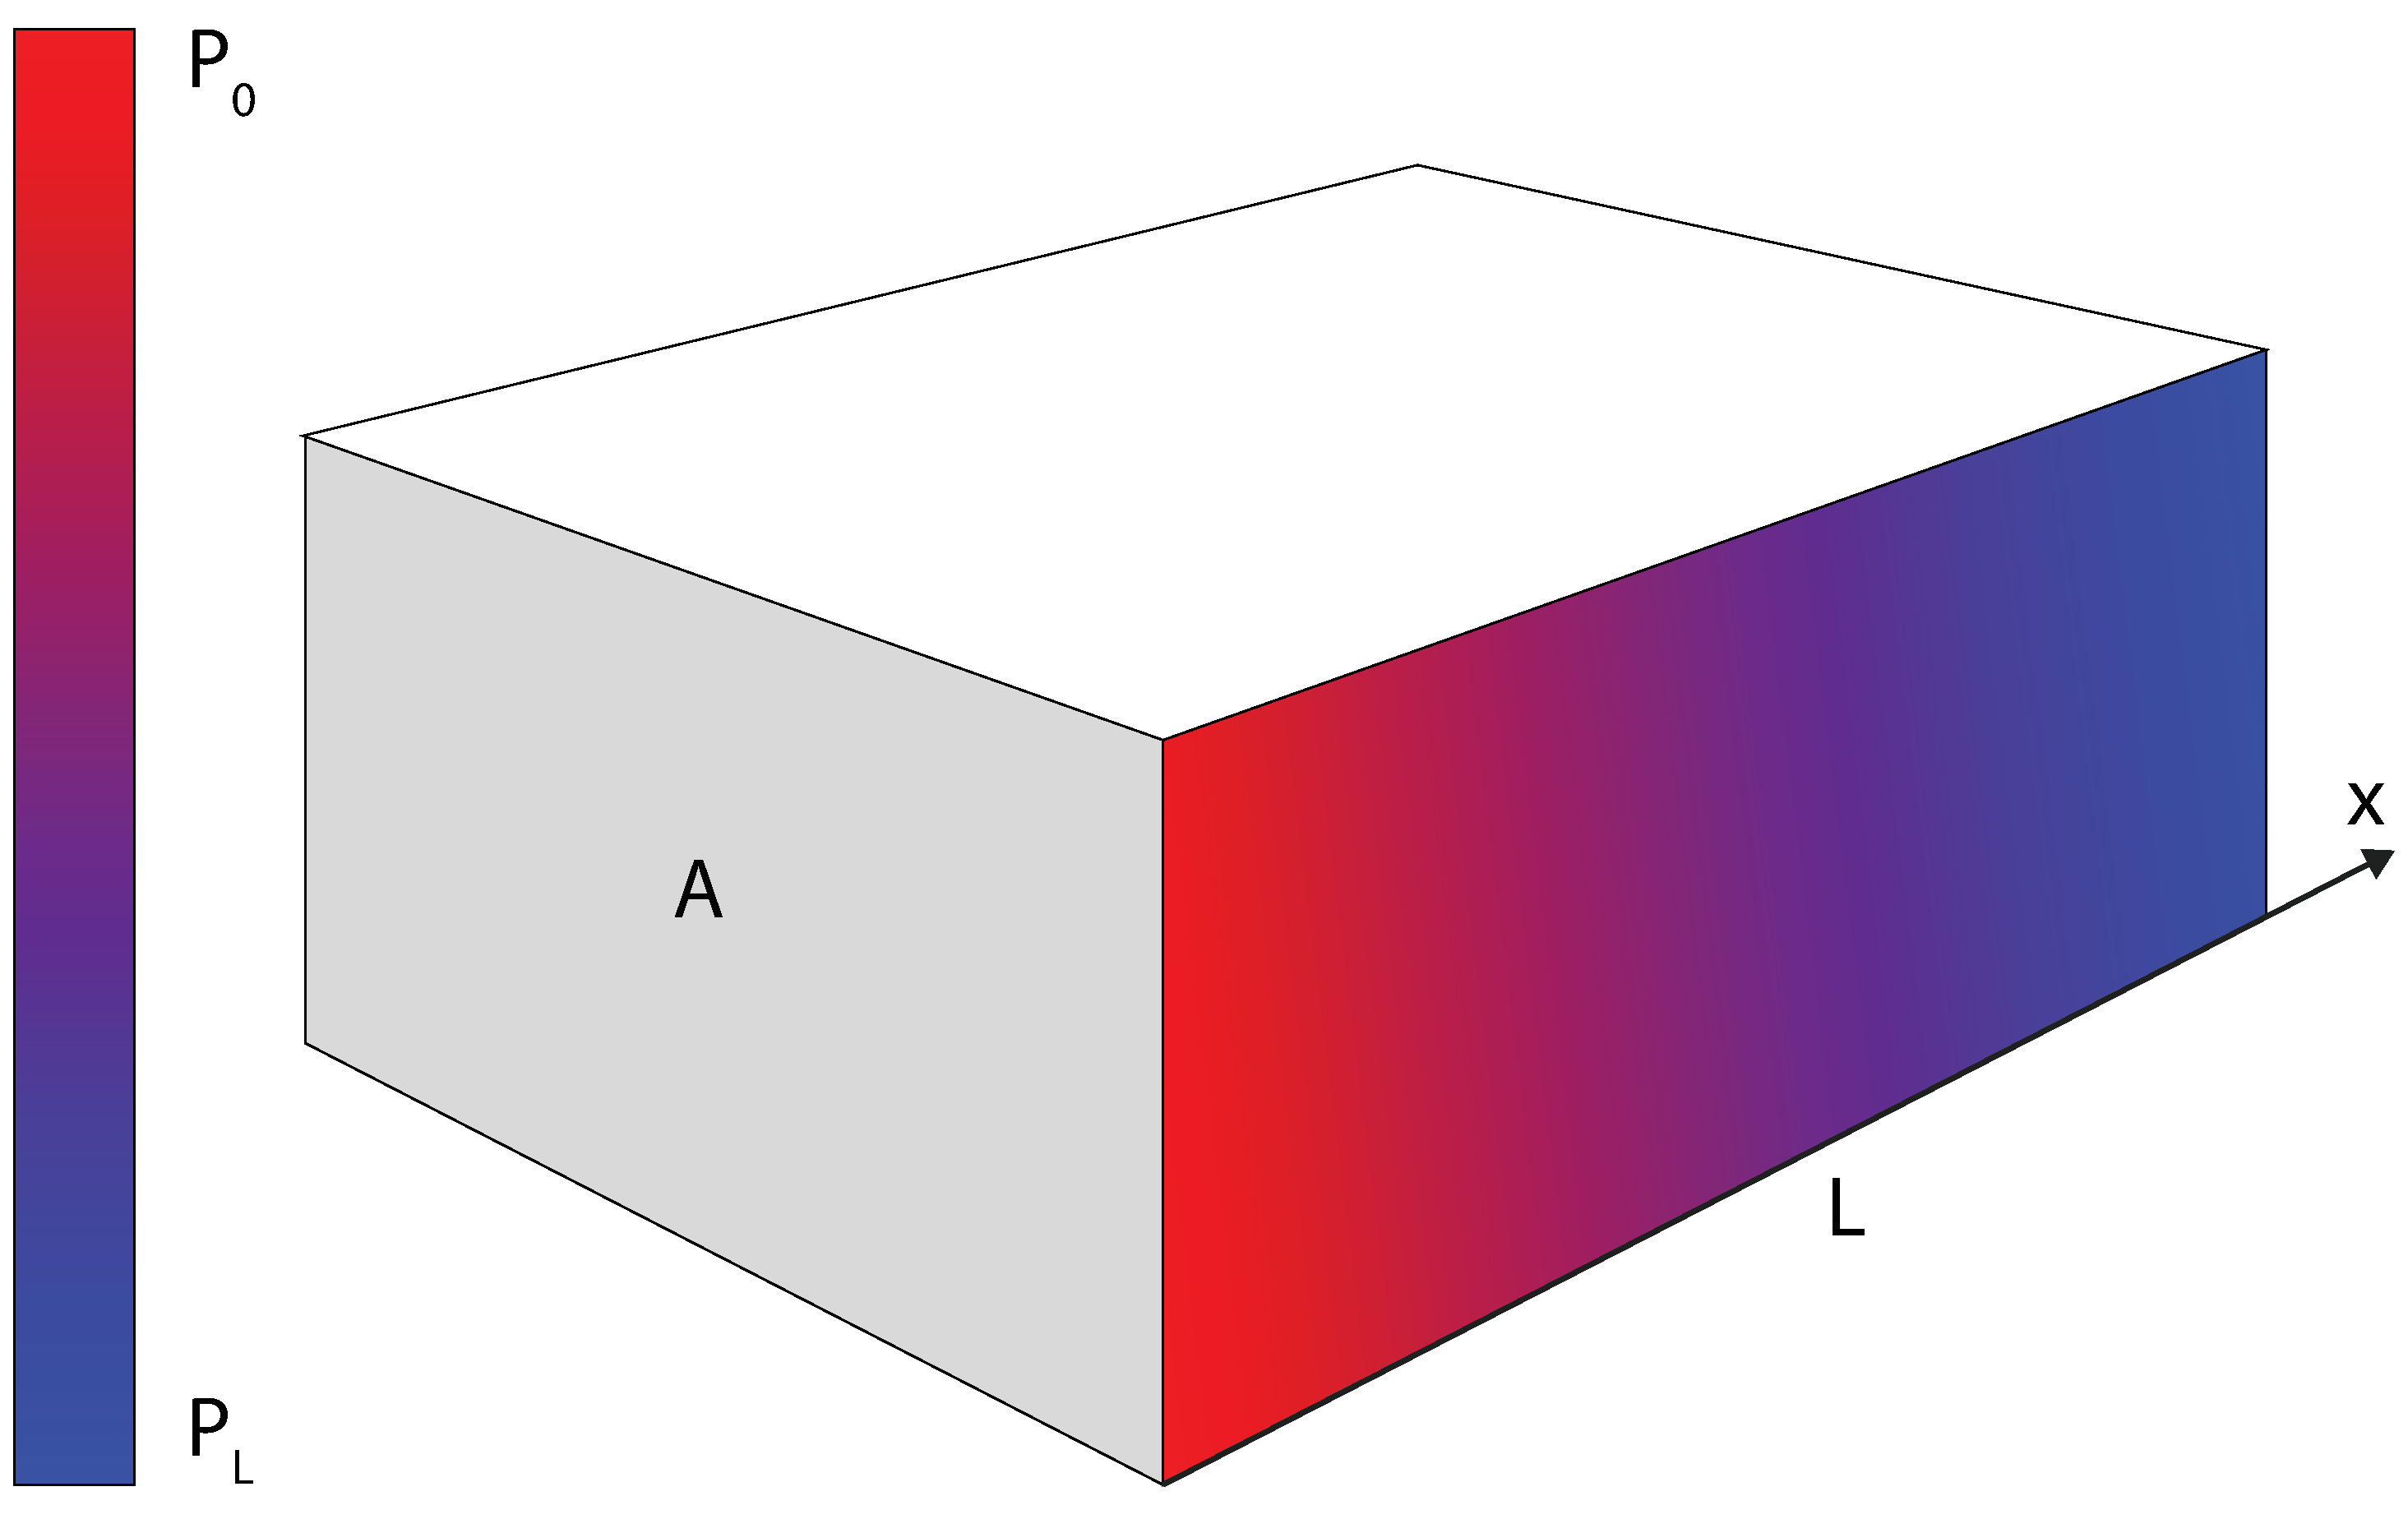
\includegraphics[width=\textwidth, trim=0cm 0cm 0cm 0cm, clip]{kinetic_theory/figures/darcy.eps}
\label{fig:darcys_law}
\end{center}
\caption{A box with volume $V=LA$ with fixed pressure values at $x=0$ and $x=L$.}
\end{figure}
Since we usually operate with flow in one direction, we will only look at the one dimensional version of Darcy's equation which is given as
\begin{align}
\label{eq:darcy_1}
	Q = A{k\over \mu}{\Delta P\over L},
\end{align}
where $A$ is the cross sectional area; the area of the plane orthogonal on the flow direction. By letting $L\rightarrow 0$, we get the differential form of Darcy's law
\begin{align}
\label{eq:darcy_2}
	Q = -A{k\over \mu}{dP\over dx},
\end{align}
where we picked up a minus sign because the fluid flows from high pressure to low pressure. One of the assumptions in the derivation of Darcy's law is that the liquid is incompressible.\cite{darcy_derivation} This is a bad approximation for gases, so we need a similar equation that allows non-constant densities. We rewrite Darcy's law by instead using the volumetric flux (or Darcy velocity) $u=Q/A$
\begin{align}
	\label{eq:darcy_3}
	u = -{k\over \mu}{dP\over dx}.
\end{align}
We then assume that the gas satisfies the ideal gas equation of state
\begin{align}
	P = \rho_n kT,
\end{align}
where $P$ is the pressure, $k_B$ is Boltzmann's constant and $T$ is the temperature. The mass continuity equation states that
\begin{align}
	\dpart{(\phi \rho_m)}{t} + \dpart{(u\rho_m)}{x} = 0,
\end{align}
which at a steady state is reduced to
\begin{align}
	\dpart{(\rho_m u)}{x} = 0,
\end{align}
which in turn gives that $\rho_m u$ is a constant and can be written as
\begin{align}
	\rho_m u = {Pm\over k_BT} c,
\end{align}
where we have applied the ideal gas law. We can solve for the Darcy velocity $u$ and insert this into equation \eqref{eq:darcy_3}
\begin{align}
	{ck_BT\over P m} &= -{k\over \mu}{dP\over dx}\\
	{ck_BT\over m}dx &= -{k\over \mu}pdP,
\end{align}
and integrate 
\begin{align}
\nonumber
	{ck_BT\over m}\int_0^L dx &= -{k\over \mu}\int_{P_0}^{P_L} pdP\\
\nonumber
	{ck_BT\over m}L &= -{k\over 2\mu}\left(P_L^2 - P_0^2\right)\\
\nonumber
	u &= {k\over 2\mu}{\left(P_0^2 - P_L^2\right)\over PL}\\
\label{eq:darcy_gas}
	Q &= A{k\over 2\mu}{\left(P_0^2 - P_L^2\right)\over PL}
\end{align}
where $u$ and $P$ is measured at the same point $x$. 

  \section{Applications}
\subsection{Shale gas extraction}
\subsection{Electronic devices}
\end{chapter}

\begin{part}{Direct Simulation Monte Carlo}
\begin{chapter}{Kinetic theory}
  The kinetic theory of gases is a microscopic theory that describes the behavior of gases on the molecular level. A system of $N$ particles is fully described by the $3N$ momentum components combined with the $3N$ spatial coordinates. Together, this forms a $6N$ dimensional phase space where each point represents the state of the system in an ensemble. We start this chapter by introducing the distribution function, the concepts of microstates, macrostates and ensembles in section \ref{sec:kinetic_theory_distribution_function}, before we in section \ref{sec:kinetic_theory_ensemble_averages} explain how we measure the macroscopic observables which are average values over all the states in an ensemble. Then we have a brief discussion about ergodicity in section \ref{sec:kinetic_theory_ergodicity} which is a very important assumption when we start measuring physical quantities in a numerical statistical mechanics model such as Direct Simulation Monte Carlo (chapter \ref{chap:dsmc}) and Molecular Dynamics (chapter \ref{chap:md}). In section \ref{sec:boltzmann_equation} we derive the Boltzmann equation which is the fundamental equation that governs the behavior of the distribution function. We then define what an equilibrium state is which we use to derive the Maxwell-Boltzmann velocity distribution in section \ref{sec:maxwell_boltzmann_distribution}. As we might remember, the Knudsen number is an important dimensionless quantity that we use to quantify how important surface and non-continuum effects are. The Knudsen number is the ratio between the mean free path $\lambda$ and some characteristic length $L$ of the system. In section \ref{sec:mean_free_path_calculation} we calculate the mean free path which is used to compute the mean collision time $\tau_\text{coll}$, which is important to choose a good timestep in the Direct Simulation Monte Carlo model in chapter \ref{chap:dsmc}.
\section{The distribution function}
\label{sec:kinetic_theory_distribution_function}
A point $(\vec r, \vec v)$ in the phase space describes what is called a \textit{microstate} and contains a massive amount of information. Given this point, we would know the position and velocity to \textit{every} particle in the entire system. In a liter of an ideal gas under standard pressure, the number of particles is of order $10^{22}$ \cite{garcia2000numerical}, so if each of these $6N$ coordinates were represented as an 8 byte \textit{double} on a computer, we would need more than $10^{11}$ terabytes of memory just to store all the information. This approach would be very inconvenient and, fortunately, not at all necessary. The really interesting properties in a system are the macroscopic ones, like energy, temperature, pressure, volume, average velocity among others. For example, the total energy in a gas consisting of $N$ particles is calculated as
\begin{align*}
	E = \sum_{i=1}^N \frac{1}{2} m_i v_i^2 + V(\vec r),
\end{align*}
where $m_i$ is the mass of particle $i$, $v_i$ is its scalar velocity and $V(\vec r)$ is the total potential energy in the system depending on the full $3N$-dimensional spatial coordinate $\vec r$.\\
Given a microstate, what happens if we switch two particles, say particle $i$ and $j$? If particle $i$ had velocity $\vec v_i = \vec u$ and particle $j$ had some other velocity $\vec v_j = \vec w$, we could quickly swap them so that $\vec v_i = \vec w$ and $\vec v_j = \vec u$ (theoretically of course, it would be a difficult task in an experiment). If their masses are identical, the total energy of the system would not change, but since \textit{we} know that we switched the two particles, we could want to count this as another microstate. We could in principle paint the particles with different colors, or maybe just label them with their own unique number. However, in a real, mono-atomic gas, we can't really tell the difference if particle $i$ and $j$ secretly agreed to switch places without telling us. If they did so, it would not count as different microstates, the system remains exactly the same. We say that the particles are \textit{indistinguishable}.\\
If we instead increase the velocity of particle $i$, we can reduce some another particle $j$'s velocity to keep the total energy constant. Even though the macroscopic property \textit{energy} is unchanged, there is a (theoretically) measurable difference between these two states. The set of all microstates that share the same macroscopic state variables (a \textit{macrostate}) forms an ensemble of systems. A much used ensemble is the microcanonical ensemble (NVE) with a constant number of particles $N$, constant volume $V$ and constant energy $E$. Increasing the velocity of particle $i$ while at the same time reducing particle $j$'s velocity just enough to remain the energy unchanged does not change the particle number $N$, the volume $V$ or the energy. So these two different microstates would both be in the same ensemble.\\

In a typical system, the number of microstates in a macrostate is so huge that the phase space points can be described by a continuous density function $f(\vec p, \vec r, t)$ without losing any important information \cite{mcquarrie1973statistical}. The input parameters are the $3N$ momentum components, the $3N$ spatial coordinates plus time. This function is often called a \textit{distribution function}, normalized so that
\begin{align}
	\iint\! f(\vec p, \vec r, t) \dm \vec p\dm \vec r = N,
\end{align}
where $\dm \vec p\dm \vec r=\dm p_1\dm p_2...\dm r_{3N}$ is the $6N$ dimensional phase space volume element. This density function does not contain the information about the \textit{exact} positions or momenta of the particles, but the \textit{probability} to find the system in a state around a given phase space point. We can then use it to calculate measurable, macroscopic average values. 

\section{Ensemble averages}
\label{sec:kinetic_theory_ensemble_averages}
Given the distribution function $f$, we can calculate any ensemble average (which will be the measurable, macroscopic properties of the system) by interpreting $f$ as a probability distribution (it needs the factor $1/N$ to be normalized to one) that gives the probability of finding a particle at position $\vec r + \dm \vec r$ with momentum in the range $\vec p + \dm\vec p$ at the time $t$. We can then use the standard expectation value expression to calculate a macroscopic property $\bar A$
\begin{align}
	\label{eq:ensemble_average}
	\bar A(t) = \frac{1}{ N}\iint\! A(\vec p, \vec r, t)f(\vec p, \vec r, t)\dm \vec p\dm\vec r.
\end{align}
This could for example be the total energy
\begin{align}
	\bar E(t) &= \frac{1}{ N}\iint\! E(\vec p, \vec r, t)f(\vec p, \vec r, t)\dm \vec p\dm\vec r \\
	&= \frac{1}{ N}\iint\! \left(V(\vec r) + \sum_{i=1}^N \frac{\vec p_i^2}{2m_i} \right)f(\vec p, \vec r, t)\dm \vec p \dm \vec r,
\end{align}
where $\vec p_i$ is the momentum of particle $i$. Any other quantity of interest can in principle be measured in the same way. 

\section{Ergodicity}
\label{sec:kinetic_theory_ergodicity}
The ensemble average calculates the average value of some macroscopic quantity given the distribution function $f$. Usually, we don't have the distribution function, except in some very simple theoretical calculations. Even then, it might be difficult to compute the integral in equation \eqref{eq:ensemble_average}. The usual situation when we do numerical statistical mechanics is that we have a way to explore the phase space, hoping that it helps us visit states with probabilities according to the given ensemble. Many Monte Carlo techniques (such as the Metropolis algorithm) allow us to go to a new, random point in the phase space, and calculate the probability of going from the current state to the new state. From this, we can count the number of times we have visited different regions of the phase space and create a histogram or maybe, if we're lucky, fit some existing probability distribution to our data.\\
Another approach is to let the rules of physics take us around in the phase space, from one state to another, following Newton's equations of motion. Imagine that at $t=0$, our system is in some microscopic state (a single phase space point ($\vec r(0), \vec p(0)$)) and at a later time $t=\tau$ has moved to ($\vec r(\tau), \vec p(\tau)$). Between these two points, the system has moved through many other points, exploring the phase space. It seems reasonable that in the limit of infinite time, the time evolution should visit the phase space points according to the density given by $f$. If not, it wouldn't make any sense even talking about $f$, since it is the time evolution we, as humans, are experiencing in the real physical world.\\
This is called the ergodicity hypothesis, the assumption that a system following the laws of physics, explores the phase space with the probability of being in a region proportional to the density in that region. The average value of a macroscopic quantity $A$ is then found as
\begin{align}
	\bar A = \lim_{t\rightarrow \infty} \frac{1}{t}\int_0^{t} A(\vec r(t'), \vec p(t'), t')\dm t'.
\end{align}
  \section{The Boltzmann equation}
\label{sec:boltzmann_equation}
In the section \ref{sec:kinetic_theory_distribution_function}, we introduced the distribution function $f$ that describes the density in a $6N$ dimensional phase space. Now, if we know the distribution function at $t=0$, we could in principle compute any property of the system. But at a later time $t=\tau$, the distribution function might have changed, unless, of course, $\partial_t f = 0$ (in which the system would be in what we call an equilibrium state). We can, by applying conservation of probability, derive an equation of motion for $f$. This equation is called the Boltzmann equation. It describes how $f$ evolves through time by assuming that any change of density (read probability) around a point $(\vec r, \vec v)$ at the time $t$ must be due to
\begin{itemize}
	\item flow through a surface in the phase space,
	\item an external force, or
	\item internal collisions.
\end{itemize}
All three will change $f$ in different ways. For simplicity, we will first assume that the particles do not collide and derive the \textit{collisionless Boltzmann equation}. But do not worry, we will add the collision term later and end up with the full Boltzmann equation.

\subsection{The collisionless Boltzmann equation}
Consider the density around the phase space point $(\vec r,\vec v)$ at the time $t$. If we assume no forces, and that the total number of particles has not changed, a time $dt$ later, the density has moved to $(\vec r + \vec vdt, \vec v)$. Conservation of probability states that any change of $f$ within a volume $\Omega$ must flow through the boundary $\partial \Omega$
\begin{align}
	\frac{\dm }{\dm t}\int_\Omega f \dm \vec r \dm \vec v &= -\int_{\Omega_v}\dm \vec v\int_{\partial \Omega_r} f(\vec v\cdot \vec n_r) \dm S_r\\
	&= -\int_{\Omega_v}\dm \vec v\int_{\Omega_r} \nabla_\vec r\cdot(f\vec v) \dm \vec r = -\int_{\Omega} \nabla_\vec r\cdot(f\vec v) \dm \vec v\dm \vec r
\end{align}
which becomes
\begin{align}
	\dpart{f}{t} + \nabla_\vec r \cdot(f\vec v) = \dpart{f}{t} + \vec v\cdot\nabla_\vec r f = 0
\end{align}
since $\vec v$ is independent of $\vec r$. We can extend this equation by adding the effects of an external force $\vec F$ that changes the velocity in the same way as the position was changed above (except for the factor $1/m$)
\begin{align}
	\label{eq:collisionless_boltzmann}
	\dpart{f}{t} + \vec v\cdot\nabla_\vec r f + \nabla_\vec v \cdot \frac{\vec F}{ m}f = 0,
\end{align}
which we call the collisionless Boltzmann equation. It is a good approximation to describe the dynamics of very dilute gases where intermolecular collisions occur rarely. But we should not ignore collisions between particles, so as promised, we will now see that by treating collisions will appear as an additional term.
\subsection{The collision operator}
We consider a dilute gas so we can assume that only binary collisions occur (we ignore the contribution from collisions between three or more particles at a time). We also assume that the total energy and momentum is conserved in all collisions. Then consider two particles $i$ and $j$ moving towards each other with velocities $\vec v$ and $\vec v_1$, and relative velocity $\vec g = \vec v - \vec v_1$. We define particle $i$ as the \textit{incident} particle and $j$ as the \textit{target} particle. After the collision, the particles will have velocities $\vec v'$ and $\vec v_1'$ with relative velocity $\vec g' = \vec v' - \vec v_1'$. In order to make the calculations simpler, we change the frame of reference. If we choose the target particle as initial frame of reference, we see that the velocity of the incident particle becomes $\tilde {\vec v} = \vec g$ and $\tilde {\vec v}' = \vec g'$. Since momentum is conserved, we know that the relative velocity must remain constant $|\vec g| = |\vec g'|$ during the collision. The direction of $\vec g'$ is given by the angles $\phi$ and $\theta$ with $\hat {\vec z}$ along $\vec g$ and $\phi \in [0, 2\pi], \theta \in [0, \pi]$. We can express $\vec g'$ as
\begin{align}
	\vec g' = \vec g - 2\unitvector e(\unitvector e\cdot\vec g),
\end{align}
where $\unitvector e$ is an arbitrary unit vector. \todo{Illustrate this with a figure?} If we multiply by $\unitvector e$, we see that 
\begin{align}
	\unitvector e\cdot \vec g' = \unitvector e\cdot\left[\vec g - 2\unitvector{e}(\unitvector e\cdot\vec g)\right] = -\unitvector e \cdot \vec g
\end{align}
which gives the symmetric relation
\begin{align}
	\vec g = \vec g' - 2\unitvector e(\unitvector e\cdot\vec g').
\end{align}
The angle between $\vec g$ and $\vec g'$ is $\theta$, so
\begin{align}
	\vec g'\cdot \vec g = g^2\cos\theta = g^2(1 - 2\cos \chi),
\end{align}
where $\chi$ is the angle between $\unitvector e$ and $\vec g$ which gives the relation
\begin{align}
	\theta = \pi - 2\chi.
\end{align}
We now define the solid angle element $\dm\Omega=\sin\theta \dm\theta \dm\phi$ about $\vec g'$ 
\begin{align}
	g \dm\Omega &= g\sin\theta \dm\theta \dm\phi = 2g\sin(\pi - 2\chi)\dm\chi \dm\phi\\
	&= 4g\cos\chi\sin\chi \dm\chi \dm\phi = 4\left|\unitvector e\cdot\vec g\right|\sin\chi \dm\chi \dm\phi\\
	&= 4\left|\unitvector e\cdot\vec g\right|\dm^2e,
\end{align}
where $\dm^2e = \sin\chi \dm\chi \dm\phi$ is a solid angle element about $\unitvector e$. In the following, we will calculate the scattering cross section which is the \textit{area} that describes the likelyhood of an incident particle being scattered by the target particle. We denote the number density $\rho_n$ and find that the incident flux is $\rho_n g$. The rate $h_{\dm\Omega}'$ of scattered particles into $\dm\Omega$ is
\begin{align}
	\label{eq:partial_scattering_rate}
	h_{\dm\Omega}' = \rho_n g\sigma \dm\Omega,
\end{align}
where the proportionality constant $\sigma$ is the cross section. We might have several target particles colliding independently of each other which will contribute to the scattering rate. If we have $n_t$ such particles, we obtain the total scattering rate $h_{\dm\Omega}$ by multiplying \eqref{eq:partial_scattering_rate} by $n_t$
\begin{align}
	h_{\dm\Omega} = n_t\rho_n g\sigma \dm\Omega.
\end{align}
The \textit{differential} cross section $\sigma$ depends on $\vec g$ and $\vec g'$, so we denote it as $\sigma = \sigma(\vec g\rightarrow \vec g')$, whereas the \textit{total} cross section $\sigma_T$ is given by integrating over all solid angles
\begin{align}
	\sigma_T = \int \sigma \dm\Omega.
\end{align}
We will now look at particles with velocities in the range $[\vec v, \vec v + \dm\vec v]$ incident on target particles with velocities in the range $[\vec v_1, \vec v_1 + \dm\vec v_1]$. The incident flux is $gf(\vec v,\vec r)\dm\vec v$ and the number of target particles is $f(v_1,\vec r)\dm\vec v_1\dm\vec r$. The rate at which particles with velocity $\vec v_1$ are scattered by particles with velocity $\vec v$ is \todo{Check if these $f$'s should be normalized}
\begin{align}
	f(\vec v)f(\vec v_1) g \sigma \dm\Omega \dm\vec v \dm\vec v_1 \dm\vec r = f(\vec v)f(\vec v_1)4\left|\unitvector e\cdot \vec g\right| \sigma \dm^2e \dm \vec v \dm\vec v_1 \dm \vec r.
\end{align}
The rate of loss is the rate of which particles in $\dm\vec v\dm\vec r$ are being hit by other particles. We can calulate this by integrating over all solid angles $\dm^2 e$ and incident velocities $\dm \vec v$
\begin{align}
	\text{rate of loss} = \left[\int f(\vec v)f(\vec v_1)4\left|\unitvector e \cdot \vec g \right|\sigma \dm^2 e\dm \vec v_1\right]\dm \vec v\dm \vec x.
\end{align}
We also have the inverse event, incident particles with velocity $\vec v'$ hitting target particles with velocity $\vec v_1'$ so that the final velocity of the target particles is $\vec v$. This is calculated with the same idea
\begin{align}
	\text{rate of gain} = \left[\int f(\vec v')f(\vec v_1')4\left|\unitvector e \cdot \vec g \right|\sigma \dm^2 e\dm \vec v_1\right]\dm\vec v\dm\vec x,
\end{align}
since $|\unitvector e\cdot \vec g| = |\unitvector e\cdot \vec g'|$ and $\dm\vec v'\dm\vec v_1' = \dm\vec v\dm\vec v_1$. The total change in the distribution function is given by the functional $J[f]$
\begin{align}
	J[f] &= \int \dm\vec v_1 \dm^2 e4|\unitvector e\cdot\vec g|\sigma[f'f_1' - ff_1]\\
	&= \int \dm\vec v_1 \dm\Omega g \sigma[f'f_1' - ff_1],
\end{align}
where $f = f(\vec r, \vec v, t)$ and $f_1 = f(\vec r, \vec v_1, t)$. The full Boltzmann equation is then given by
\begin{align}
	\label{eq:boltzmann_equation}
	\dpart{f}{t} + \vec v\cdot \nabla_\vec r f + \frac{\vec F}{m}\cdot\nabla_\vec v f = J[f].
\end{align}
In the derivation of the collision operator $J[f]$, we assumed binary collisions only. This is a decent approximation that holds for low densities. By defining the force range $D$ and the dimensionless parameter $\nu = \rho_n D^3$, the Boltzmann equation is valid when $\nu$ is small \cite{mclennan1989introduction}. $D^3$ defines a volume around a particle in which the forces cannot be neglected. This makes $\nu$ the average number of particles within that volume. If that number is small (less than unity) then we can safely neglect collisions between three or more particles.
\section{\textit{H}-theorem}

Boltzmann's $H$-theorem is a powerful result that gives us all the theoretical tools we need to implement the DSMC method. We define the $H$-function as
\begin{align}
	H(t) = \langle \ln f \rangle = \int f(\vec r, \vec v, t)\ln f(\vec r, \vec v, t)d\vec r d\vec v
\end{align}
and differenciate with respect to time
\begin{align}
	\frac{dH}{dt} = \int \dpart{f}{t}\ln f d\vec r d\vec v + \int \dpart{f}{t} d\vec r d\vec v = \int \dpart{f}{t}\ln f d\vec r d\vec v
\end{align}
where we have used that the number of particles is conserved
\begin{align}
	\int \dpart{f}{t}d\vec r d\vec v = \frac{d}{dt} \int fd\vec r d\vec v = \frac{dN}{dt} = 0.
\end{align}
We multiply the Boltzmann equation by $\ln f$ and integrate
\begin{align}
	% \int \dpart{f}{t}\ln f d\vec r d\vec v = -\int (\ln f)\vec v\cdot \nabla_\vec r f d\vec r d\vec v - \int (\ln f) {\vec F\over m}\cdot \nable_\vec v f d\vec rd\vec v + \int \ln f J[f] d\vec r d\vec v
	balle
\end{align}

\section{Maxwell-Boltzmann distribution as equilibrium}
\label{sec:maxwell_boltzmann_distribution}
\begin{align}
	\label{eq:maxwell_boltzmann_distribution}
	P(v_i)\dm {v_i} = \sqrt\frac{m}{ 2\pi k_BT}e^\frac{-mv_i^2}{ 2k_BT}\dm {v_i},
\end{align}
\section{Mean free path}
\label{sec:mean_free_path_calculation}
The collision frequency can be calculated through the mean free path, which is the average distance a molecule travels between collisions. The mean free path for a gas is estimated by looking at the \textit{effective collision area}, see figure \ref{fig:effective_collision_area}. The effective collision area is then
\begin{align}
	A = \pi d^2,
\end{align}
where $d$ is the molecular diameter. Two molecules with velocities $\vec v_1$ and $\vec v_2$ have the relative velocity $\vec v_{rel} = \vec v_1 - \vec v_2$. The norm is given by
\begin{align}
	v_{rel} &= \sqrt{\vec v_{rel}\cdot \vec v_{rel} } = \sqrt{ (\vec v_1 - \vec v_2)(\vec v_1 - \vec v_2)}\\
	&= \sqrt{\vec v_1\cdot \vec v_1 - 2\vec v_1\vec v_2 + \vec v_2\vec v_2}.
\end{align}
The average relative velocity is calculated by assuming that the velocities are completely random and hence not correlated, and that the molecules have the same mean speed $\langle v\rangle$
\begin{align}
	\bar v_{rel} &= \sqrt{\vec v_1^2 + \vec v_2^2} = \sqrt 2 \langle v\rangle,
\end{align}li
During a time $\tau$ and average relative molecular velocity $\sqrt 2 \langle v\rangle$, the total volume sweeped out by the particle is given as
\begin{align}
	V = \sqrt 2 \pi d^2\langle v\rangle \tau,
\end{align}
which in turn gives the number of collisions during such a volume
\begin{align}
	\label{eq:num_collisions}
	n_{coll} = V\rho_n = \sqrt 2 \pi d^2\langle v\rangle \rho_n \tau,
\end{align}
where $\rho_n$ is the number density. The mean free path is then calculated as the length of the path divided by the number of collisions
\begin{align}
	\label{eq:mean_free_path}
	\lambda = \frac{\langle v\rangle \tau}{ \sqrt 2 \pi d^2\langle v\rangle \rho_n\tau} = \frac{1 }{ \sqrt 2 \pi d^2 \rho_n}
\end{align}
\section{Mean collision time}
\begin{align}
	\label{eq:coll_frequency}
	f_{coll} = \rho_n \pi \sigma^2 \langle v_r \rangle
\end{align}
\end{chapter}

\begin{chapter}{Introduction}
  \label{chap:dsmc}
  We now have the theoretical foundation we need to develop the first numerical model we will use to study flow in nanoporous media. It is called Direct Simulation Monte Carlo (DSMC), and is a stochastic particle model that has showed incredible predictive power for flow in the high Knudsen number regime. The model was developed by G. A. Bird in 1976 and was quickly picked up by engineers working in the field of aerospace. In the upper atmosphere (\unit{100}{\kilo\meter}), the mean free path of air is several meters. For space shuttles, this gives a Knudsen number of order unity since the size of its nose is of order meter \cite{alexander1997direct}. In the later years, the method has been widely used to study microflows which is our main concern in this thesis. In 1992, the model was proved to converge towards a solution of the Boltzmann equation (equation \eqref{eq:boltzmann_equation}) in the limit where the timestep $\Delta t\rightarrow 0$ and the number of particles $M\rightarrow \infty$.\\
We start the chapter by introducing the model and its basic philosophy. The model has two two crucial parts, collisions between particles which is discussed in section \ref{sec:dsmc_collisions_model}, and how the particles interact with the surface. The latter is covered in section \ref{sec:surface_interactions}. Another important subject is of course how we measure physical quantities like temperature and energy. This is described in section \ref{sec:dsmc_measuring_physical_quantities}. In section \ref{sec:dsmc_pressure} we have a longer discussion about the pressure and argue that a DSMC gas actually satisfies the ideal gas equation of state. We also derive a relationship between a given pressure difference $\Delta P$ and a constant force allowing us to induce flow in the system without needing large gradients in the density or temperature. We then have a brief comment about the numerical stability and how the timestep and collision cell size introduce errors in transport coefficients. We complete the chapter by discussing how we determine whether or not a system has reached a steady state in section \ref{sec:dsmc_steady_state}. The implementation of all these steps are explained in detail in chapter \ref{chap:dsmc_implementation}.
  \section{The model}
The Direct Simulation Monte Carlo
\subsection{Intermolecular collision}
The collision frequency can be calculated through the mean free path, which is the average distance a molecule travels between colisions. The mean free path for a gas is estimated by looking at the \textit{effective collision area}, see figure \ref{fig:effective_collision_area}. The effective collision area is then
\begin{align}
	A = \pi d^2,
\end{align}
where $d$ is the molecular diameter. Two molecules with velocities $\vec v_1$ and $\vec v_2$ have the relative velocity $\vec v_{rel} = \vec v_1 - \vec v_2$. The norm is given by
\begin{align}
	v_{rel} &= \sqrt{\vec v_{rel}\cdot \vec v_{rel} } = \sqrt{ (\vec v_1 - \vec v_2)(\vec v_1 - \vec v_2)}\\
	&= \sqrt{\vec v_1\cdot \vec v_1 - 2\vec v_1\vec v_2 + \vec v_2\vec v_2}.
\end{align}
The average relative velocity is calculated by assuming that the velocities are completely random and hence not correlated, and that the molecules have the same mean speed
\begin{align}
	\bar v_{rel} &= \sqrt{\vec v_1^2 + \vec v_2^2} = \sqrt 2 \bar v,
\end{align}
During a time $\tau$ and average relative molecular velocity $\sqrt 2 \bar v$, the total volume sweeped out by the particle is given as
\begin{align}
	V = \sqrt 2 \pi d^2\bar v \tau,
\end{align}
which in turn gives the number of collisions during such a volume
\begin{align}
	n_{coll} = V\rho_n = \sqrt 2 \pi d^2\bar v \tau \rho_n,
\end{align}
where $\rho_n$ is the number density. The mean free path is then calculated as the length of the path divided by the number of collisions
\begin{align}
	\lambda = {\bar v \tau\over \sqrt 2 \pi d^2\bar v \tau \rho_n} = {1 \over \sqrt 2 \pi d^2 \rho_n}
\end{align}
\section{Large systems}
  \section{Surface interactions}
\label{sec:surface_interactions}
The effects of surface interactions become significant as the pore sizes decrease. For very small pores, the number of atoms near the surface is comparable with total number of atoms. In MD, these effects are already taken care of through the atomic forces, but in DSMC, we need a surface interaction model. We discuss three different models in this section. The main property of these models is to perform a statistically correct energy and momentum transfer between the wall and the colliding particles. In DSMC, we are only interested in the macroscopic details of these collisions. There are two important parameters that incorporates the differences between different gases and surfaces; the normal and tangential accomodation coefficients.
\subsection{Accomodation coefficients}
When a particle hits a wall with energy $E_i$, some of the energy might be transferred to the wall resulting in an energy change $\Delta E$. On average, we can define the \textit{normal accomodation coefficient} 
\begin{align}
	\sigma_n = \frac{E_i - E_r}{E_i - E_w},
\end{align}
where $E_i$ is the energy of the incoming particles, $E_r$ is the energy of the outging molecules and $E_w$ is the energy corresponding to the surface temperature $T_w$. A thermal accomodation coefficient equal to zero would mean that there is no energy exchange, and we will get the specular wall model described below. $\sigma_T=1$ on the other hand means that all the reflected particles have energies corresponding to the surface temperature. This is what we call the thermal wall (or diffuse reflection\cite{karniadakis2005microflows}), and there is no correlation between the incoming and outgoing velocities. More intricate models make use of other values of the accomodation coefficients so the particles \textit{remember} their incoming velocities.\\
We can also define the \textit{tangential momentum accomodation coefficient}
\begin{align}
	\sigma_t = {\tau_i - \tau_r\over \tau_i - \tau_w},
\end{align}
where $\tau_i$ and $\tau_r$ are the incoming and outgoing tangential momentum and $\tau_w$ is the momentum of the wall. For stationary surfaces we have $\tau_w=0$.

\subsection{Specular wall}
The specular wall behaves just like a classical mirror. The colliding objects are reflected so that the normal component of the velocity is reversed while the tangential components remain unchanged. There is no exchange of energy with the wall. 

\subsection{Thermal wall}
If we instead think of the wall as an object with a given temperature $T_w$, we can imagine that the particles go into the wall, collide with the wall atoms as a random walk, and return with no correlation with the incoming velocity. We can then choose a new, random velocity vector from a distribution so that the gas temperature converges to the wall temperature. This distribution has to reflect the fact that faster particles collide more often with the surface. A distribution that satisfies this property is the biased Maxwell-Boltzmann distribution given as
\begin{align}
	P_n(v_n) = {m\over kT_w}v_n e^{-mv_n^2/2kT_w}
\end{align}
for the velocity component normal on the surface and
\begin{align}
	P_t(v_t) = \sqrt{m\over 2\pi kT_w}e^{-mv_t^2/2kT_w},
\end{align}
for the tangential component. Here $m$ is the mass of the particle and $k$ is Boltzmann's constant\cite{alexander1997direct}. This distribution does not obey detailed balance since the incoming velocity is completely uncorrelated to the outgoing velocity. It is computationally inexpensive and is much used in the literature. 
\subsection{The Cercignani-Lampis model}
Another more realistic model is the Cercignani-Lampis model which was derived requiring detailed balance and wall isotropy\cite{cowling1974cercignani}. The probability of going from an incoming velocity $\vec v'$ to an outgoing velocity $\vec v$ is given as
\begin{align}
	\nonumber
	P(\vec v'\rightarrow \vec v) &= \frac{2\sigma_n\sigma_t(2-\sigma_t)\beta_w^4}{\pi}\\
	\nonumber
	&\times\exp\Big(-\beta_w^2\frac{v_n^2 + (1-\sigma_n)(v_n')^2}{\sigma_n} - \beta_w^2\frac{(v_t - (1 - \sigma_t)v_t')^2}{\sigma_t(2 - \sigma_t)}\Big)\\
	&\times I_0\Big(\beta_w^2\frac{2\sqrt{1 - \sigma_t}v_nv_n'}{\sigma_n}\Big),
\end{align}
where $v_n$ and $v_t$ are the normal and tangential components of the velocities, $I_0$ is the zeroth-order modified Bessel function of the first kind. We see that the tangential component is a normal distribution with a non-zero mean, whereas the normal component is more complicated. The distribution for the normal component is plotted in figure \ref{fig:cercignani_lampis}.

\begin{figure}[h]
\begin{center}
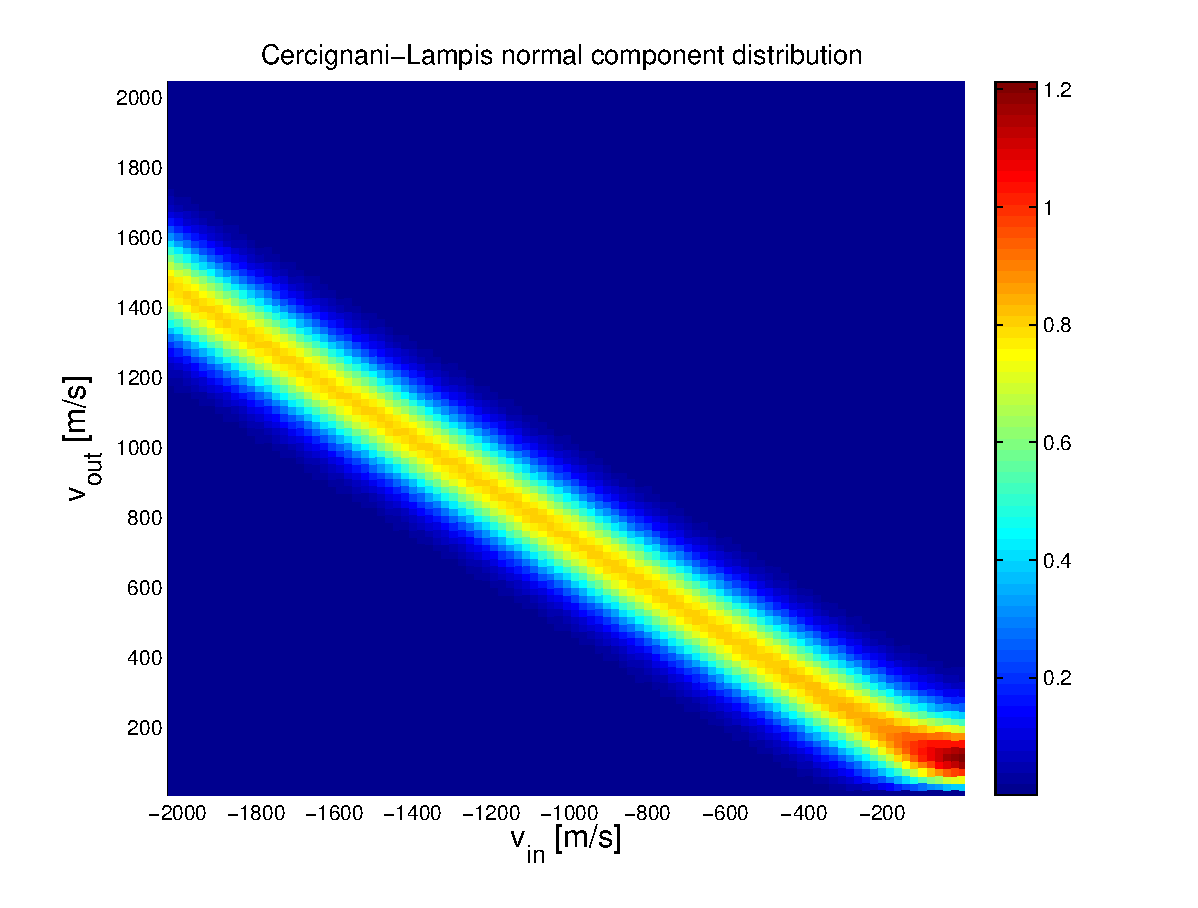
\includegraphics[width=\textwidth, trim=0cm 0cm 0cm 0cm, clip]{DSMC/figures/cercignani-lampis.eps}
\label{fig:cercignani_lampis}
\end{center}
\caption{The Cercignani-Lampis normal component distribution for $T=100K$, $m=m_{argon}$, $\alpha_n=0.5$. We see that particles with high velocities are reflected with a slightly lower velicities converging towards the velocity corresponding to the wall temperature $T_w$.}
\end{figure}

To draw random numbers from this distribution is orders of magnitudes more expensive than the thermal wall since it isn't trivial to invert the cumulative distribution function. Instead we must use the von Neumann algorithm which is a Monte Carlo technique\cite{allen1989computer}. I have implemented and tested this method, but due to the computational cost, the main focus in this thesis is the thermal wall which is used in all the results. 
  \section{Physical properties}
Once the simulation program is written, we can create states with all the information needed to know any physical property about the system. However, most macroscopic quantities are of statistical nature and require a time average in a steady state to reach the real expectation value. 
\subsection{Steady state}

\subsection{Energy}
The total energy of a system is as usual given by the sum of the kinetic and potential energy. Since we are using the hard sphere model, we remember that the potential energy is given as
\begin{align}
	V(\vec r_1, \vec r_2) = \left\{
	\begin{array}{lr}
	0 & \text{if} |\vec r_1  - \vec r_2| \leq d\\
	\infty & \text{if} |\vec r_1  - \vec r_2| < d\\
	\end{array}
	\right .
\end{align}
where collisions will make sure that the relative distance between any particle pair always remains larger than the diameter. The total energy of our entire system will then be the kinetic energy
\begin{align}
	E = E_K = \sum_{n=1}^N {1\over 2}m_iv_i^2
\end{align}
where $m_i$ is the mass of particle $i$ and $v_i$ is its scalar velocity. An example implementation of how the kinetic energy is calculated is given in listing \ref{lst:dsmc_kinetic_energy}. Remember that in DSMC, each particle represents a given number of real atoms.

\begin{lstlisting}[caption=Calculation of kinetic energy., label=lst:dsmc_kinetic_energy]
double calculate_kinetic_energy(vector<vector<double> > &velocities, vector<double> &masses, int atoms_per_particle) {
	double kinetic_energy = 0;
	int num_particles = velocities.size();
	for(int i=0; i<num_particles; i++) {
		vector<double> &velocity = velocities.at(i);
		double velocity_squared = velocity.at(0)*velocity.at(0) + velocity.at(1)*velocity.at(1) + velocity.at(2)*velocity.at(2);
		double mass = masses.at(i);
		kinetic_energy += 0.5*mass*atoms_per_particle*velocity_squared;
	}

	return kinetic_energy;
}
\end{lstlisting}

\subsection{Temperature}
The temperature is defined through the equipartition theorem using the three momentum degrees of freedom
\begin{align}
	\langle E_k \rangle = {3\over 2}NkT,
\end{align}
where $\langle E_k \rangle$ is the average kinetic energy, $N$ is the number of particles, $k$ is Boltzmann's constant and $T$ is the temperature. The only unknown property in this equation is the temperature
\begin{align}
	T = \frac{2E_k}{3Nk},
\end{align}
where we have dropped the average value brackets of the kinetic energy because we use this to define the \textit{instantaneous} temperature which in turn must be averaged in order to get the actual gas temperature over time. In listing \ref{lst:dsmc_temperature}, we show how to calculate the temperature in a DSMC model.

\begin{lstlisting}[caption=Calculation of instantaneous temperature., label=lst:dsmc_temperature]
double calculate_temperature(vector<vector<double> > &velocities, vector<double> &masses, int atoms_per_particle) {
	double kinetic_energy = calculate_kinetic_energy(velocities, masses, atoms_per_particle);
	int num_particles = velocities.size();
	int num_real_atoms = num_particles*atoms_per_particle;
	
	double temperature = 2*kinetic_energy / (3*num_real_atoms*boltzmann_constant);
	
	return temperature;
}
\end{lstlisting}

\subsection{Pressure}

\subsection{Density}
\subsection{Permeability}
  \section{Numerical stability and discretization error}
\label{sec:dsmc_stability}
Most numerical methods have a critical stability criterion where the energy or some other property might diverge if the timestep is too large. For example, while solving PDE's with a finite difference scheme, we often encounter the Courant number which is a critical threshold of the ratio of the discretization length of space and time. For the one-dimensional wave equation, this can be expressed as
\begin{align}
	C = \frac{|\dot x|_{max} \Delta x}{\Delta t} \leq C_{max},
\end{align}
where $|\dot x|_{max}$ is the magnitude of the velocity. If the spatial grid has high resolution, small $\Delta x$, we need a similarly small timestep $\Delta t$.

However, since the DSMC model always conserves energy and momentum (during particle collisions), the method is in principle numerically stable for any timestep. As mentioned in section \ref{sec:dsmc_model}, the timestep is split into two parts; moving and colliding. The timestep should therefore be smaller than the mean collision time. Larger timesteps may result in large errors in the transport coefficients (such as viscosity and thermal conductivity)\cite{karniadakis2005microflows}. While the timestep is compared to the mean collision time $\tau_\text{coll}$, the collision cell size can be seen as the spatial discretization, and be compared to the mean free path $\lambda$. 
\subsection{Finite cell size}
The collision cells allows all particles within a cell to collide with each other. So if the cell size is very large, particles from a hot region (in one corner of the collision cell) may collide with particles in a colder region (maybe in another corner) that are displaced by a large distance. This could enable heat to transfer much faster than it would in a real gas. The cell size $L_\text{cell}$ should therefore at least be smaller than the mean free path\cite{karniadakis2005microflows}. The viscosity can be calculated from kinetic theory
\begin{align}
	\mu = \frac{5}{16d^2}\sqrt{\frac{mk_B T}{\pi}},
\end{align}
which Garcia et al. \cite{alexander1998cell} used to show that the error in the viscosity has a quadratic dependency of the cell size
\begin{align}
	\label{eq:viscosity_cell_size}
	\mu(L_\text{cell}) = \frac{5}{16d^2}\sqrt{\frac{mk_B T}{\pi}} \left [1 + \frac{16}{45\pi}\frac{L_\text{cell}^2}{\lambda^2}\right].
\end{align}
If the length of the collision cells equals the mean free path, we could then expect a $~10\%$ error in the viscosity coefficient.
\subsection{Finite timestep}
A large timestep may allow particles to travel through several collision cells during a single timestep. This would allow information to travel faster than in a real gas and also leads to errors in transport coefficients like the viscosity. Hadjiconstantinou \cite{hadjiconstantinou2000analysis} derived an expression for the timestep dependency for the viscosity, similar to equation \eqref{eq:viscosity_cell_size}
\begin{align}
	\mu = \frac{5}{16d^2}\sqrt{\frac{mk_B T}{\pi}} \left [1 + \frac{16}{75\pi}\frac{(v_m\Delta t)^2}{\lambda^2}\right],
\end{align}
where $v_m=\sqrt{2k_B/mT}$ is the most probable velocity. We see that the error is proportional to $(v_m\Delta T/\lambda)^2$ which vanishes in the limit $\Delta t\rightarrow 0$. 
  \section{Equation of state}
\label{sec:dsmc_eos}
The free \textit{modules} in a DSMC simulation are the collision operator $\mathcal C$ and the move operator $\mathcal M$ which fully (stochastically) determines the time evolution of the system. For hard sphere particles, the pressure may be defined in a similar way as for MD (equation \eqref{eq:pressure_in_md})
\begin{align}
	P = \rho_nkT + {1\over tV}\sum_\text{all collisions} m\Delta \vec v_{ij}\cdot \vec r_{ij},
\end{align}
where $\Delta \vec v_{ij}$ is the change of velocity of one of the particles during a collision and $\vec r_{ij}$ is the distance between these two particles\cite{garcia1997direct}. If we choose the hard sphere collision model as described in section \ref{sec:dsmc_collisions_model}, there is no correlation between the change in velocity $\Delta \vec v_{ij}$ and the displacement vector $\vec r_{ij}$
\begin{align}
	\langle \Delta \vec v_{ij}\cdot \vec r_{ij}\rangle = 0,
\end{align}
so the expression for the pressure is reduced to that of ideal gas
\begin{align}
	P = \rho_n kT.
\end{align}
Since the main focus of this thesis is to study dilute gases where the ideal gas is a good approximation, this collision model is sufficient enough. For dense gases, it is possible to apply collision models that yields other equations of state.
\subsection{Non-ideal gas corrections}
  \subsection{Measuring permeability}
\label{sec:permeability_acceleration_driven}
\todo{Here also, use the $\rho g$ version of darcy's law}
The permeability was defined in section \ref{sec:permeability_dsmc} through Darcy's law (equation \eqref{eq:darcy_1})
\begin{align}
	k = \frac{Q\mu L}{A \Delta P},
\end{align}
but we did not know how to correctly evaluate the pressure since $x=0$ is the same point as $x=L$ in a periodic system with length $L$. We can define the pressure at $x=0$ through the ideal gas law, and due to the acceleration $g$ there is an implied pressure at $x=L$ we can find by using equation \eqref{eq:acceleration_to_pressure_difference}
\begin{align}
	P_0 &= \rho_n(x=0)kT\\
	P_L &= P_0 - \Delta P \\
	&= \rho_n(x=0)kT - \bar{\rho}_m g L,
\end{align}
where $\bar{\rho}_m$ is the average density in the system and we have used that $\Delta x=L$.\\
We still need to figure out how to measure the volumetric flow rate $Q$. The volumetric flow rate tells us how much volume that passes through a surface per time. The simplest way to measure $Q$ is to count how many particles that have passed through a surface and multiply that number with the volume per particle $\rho_n^{-1}$. Since we apply periodic boundary conditions on particles that fly out of the system, we just have to keep track of how many, this is illustrated in listing \ref{lst:dsmc_apply_periodic_boundary_conditions}.
\begin{lstlisting}[caption=Example of how to apply periodic boundary conditions and at the same time calculate number flux., label=lst:dsmc_apply_periodic_boundary_conditions]
void apply_periodic_boundary_conditions(vector<double>&position, vector<long> &count_periodic, vector<double> &system_length)
{
    if(position[0] >= system_length[0]) { 
    	position[0] -= system_length[0]; count_periodic[0]++; 
    }
    else if(position[0] < 0) { 
    	position[0] += system_length[1]; count_periodic[0]--; 
    }

    if(position[1] >= system_length[1]) { 
    	position[1] -= system_length[1]; count_periodic[1]++;
    }
    else if(position[1] < 0) {
    	position[1] += system_length[1]; count_periodic[1]--; 
    }

    if(position[2] >= system_length[2]) { 
    	position[2] -= system_length[2]; count_periodic[2]++; 
    }
    else if(position[2] < 0) {
    	position[2] += system_length[2]; count_periodic[2]--; 
    }
}
\end{lstlisting}
Now that we have the number flux, we can easily calculate the permeability as shown in listing 
\begin{lstlisting}[caption=Calculation of permeability\, assuming that flow is in the $z$-direction., label=lst:dsmc_permeability]
double calculate_permeability(double volume, long num_particles, double viscosity, vector<long> &count_periodic, vector<double> &system_length, double mass_density, double acceleration)
{	
    double volume_per_particle = volume / num_particles;

    // We assuming that the flow is in z-direction
    double volume_flow_rate = count_periodic[2]*volume_per_molecule;
    double area = system_length[0]*system_length[1];

    double pressure_0 = system->density*system->temperature;
    double pressure_L = pressure_in_reservoir_0 - mass_density*acceleration*system_length[2];
    double permeability = 2*pressure_0*volume_flow_rate*system_length[2]*viscosity / (area * (pressure_0*pressure_0 - pressure_L*pressure_L));

    return permeability;
}
\end{lstlisting}
  \section{Reaching a steady state}
\label{sec:dsmc_steady_state}
Since we want to study flow in nanoporous media, before inducing the flow, the fluid is on average obviously at rest. Immediately after we have started applying the constant force that will make the fluid flow, the fluid velocity is still approximately zero. After a certain amount of time, the system will reach a steady state which in its most simple form can be defined as when the time derivative of the \textit{fluid velocity} in any region, the local velocity, is zero. We should not start to sample flow statistics like the permeability until such a state has been reached. However, the system may not be in a steady state even though the average local fluid velocity does not change over time. There are other physical quantities like that may still be changing.\\
A naive, but simple approach to measure whether or not the fluid velocity has converged is to look at the measured temperature defined in equation \eqref{eq:dsmc_temperature}. If the gas temperature starts out at $T= $\unit{300}{\kelvin} before the flow is induced, the measured temperature will increase while the fluid velocity increases. Once the fluid has reached a steady state, the temperature will have converged to some value it will continue fluctuating around. For simplicity, this is how we have determined whether or not the system has reached the steady state. In future development of the code, better methods should be implemented.
\end{chapter}
\begin{chapter}{Implementation}
  In this chapter we go into detail about how the DSMC model is implemented in c++. We assume that the reader is familiar with c++ and object orientation. First, we discuss how the code is object oriented and how the different classes are structured. We will explain how particles are divided into collision cells and how the collisions are calculated. The algorithm for detecting and performing surface interactions is discussed, in addition to how the code is parallelized with Message Passing Interface (MPI).


\section{Code structure and variables}
The main function of the program initiates an instance of the class \textit{System} which is the main class of the simulator. It also has an object of the \textit{SystemSampler} class that samples the physical quantities following the definitions in section \ref{sec:dsmc_measuring_physical_quantities}. In this section we go through all of the classes and how they are connected (as shown in figure \ref{fig:dsmc_uml_diagram}). 
\begin{figure}[h]
\begin{center}
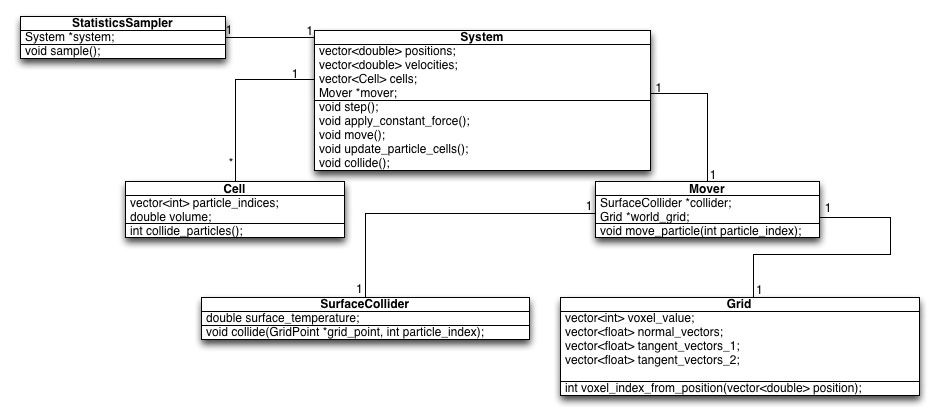
\includegraphics[width=\textwidth, trim=0cm 0cm 0cm 0cm, clip]{DSMC/figures/dsmcuml.png}
\end{center}
\caption{A UML-diagram showing how the classes in the DSMC program are related to each other.}
\label{fig:dsmc_uml_diagram}
\end{figure}
\subsection{main.cpp}
The main function is of course the top level scope of the program. It creates the objects used to read settings, simulate the system and sample statistics. The code is summarized in listing \ref{lst:dsmcmaincpp}.
\begin{lstlisting}[caption=main.cpp, label=lst:dsmcmaincpp]
int main(int args, char* argv[]) {
    // Initialize MPI
    Settings settings("dsmc.ini");
    System system;
    system.initialize(&settings, myid)
    StatisticsSampler sampler(&system);
    
    // Load data from earlier timestep

    for(int timestep=0;timestep<settings.timesteps;timestep++) {
    	system.step();
    	sampler.sample();
    }

    // Save data to file
    // Finalize
}
\end{lstlisting}
\subsection{Class System}
The system class is the top level simulator class. It reads all the physical properties of the system (i.e. system size, density, world geometry) and executes each timestep when it's asked to do so. The phase space variables are saved in 
\begin{itemize}
\item \textit{std::vector<double> r}
\item \textit{std::vector<double> v}
\end{itemize}
  \section{Collision cells}
\label{sec:dsmc_collision_cells}

  \section{Complex geometries}
\label{sec:dsmc_complex_geometries}
All the surface interaction models from section \ref{sec:surface_interactions} use the surface normal and tangent vectors to calculate the reflected velocities. These vectors are easy to determine if the system consists of two parallel plates in the xy-plane, or any other mathematically well described geometry. Such systems are interesting as validation test cases, but most real world materials have a more complex geometry without any simple mathematical description. A very much used representation of such geometries is a triangle mesh in which the surface consists of many connected triangles. The triangles have a well defined normal vector and tangent plane which is easy to calculate. With this method, collision detection is done by checking intersection with each triangle and is rather computationally expensive. In this thesis, I have chosen another approach by representing the system as a large, binary three-dimensional matrix consisting of voxels, each having the value \textit{filled} or \textit{empty}. With this model, collision detection is done by a quick memory lookup to check if the voxel corresponding to the position of a particle is filled or not. In this section we discuss how to create such a matrix, how to identify the surface points and how to calculate the vectors describing the surface geometry.

\subsection{Binary representation - voxels}
\label{sec:dsmc_binary_representation}
With this method, any system geometry is fully described by a three dimensional matrix with dimensions $m\times n\times l$. Each matrix element represents a voxel in the physical space, and can take values 0 or 1. A value of one means that the voxel is filled, whereas zero means empty. No particles can be inside a filled voxel, so this is how we do surface collision detection. 
\subsection{Collision detection}
We define a collision as whether or not a particle has moved into a wall during the timestep $\Delta t$. This has to be checked for every particle each timestep, and in the case of a collision, we need to calculate the resultant velocity. The collision detection algorithm is best illustrated by a code example:
\begin{lstlisting}
bool did_collide(double *position) {
	int voxel_index_i = position[0] / system_length[0] * num_voxels[0];
	int voxel_index_j = position[1] / system_length[1] * num_voxels[1];
	int voxel_index_k = position[2] / system_length[2] * num_voxels[2];

	// The world matrix is a binary matrix
	return world_matrix[voxel_index_i, voxel_index_j, voxel_index_k];
}
\end{lstlisting}
This is just a quick memory lookup. The really expensive part of the full collision algorithm is finding exactly which voxel is the first surface voxel the particle hits. We need to precalculate all the surface voxels so they are marked in the matrix during runtime.
\subsection{Identifying the surface voxels}
Given the binary matrix, we have identified every solid part of the system. The voxels inside a wall that are not part of the surface all have neighbouring voxels that are also marked as walls. We \textit{define} the surface as the filled voxels that have less than 26 neighbouring filled voxels. The algorithm could be implemented like this (one would also have to take care of the periodic boundary conditions, but that is not important to illustrate the idea):
\begin{lstlisting}
bool is_surface(short ***world_matrix, int voxel_index_i, int voxel_index_j, int voxel_index_k) {
	for(int i=-1;i<1;i++) {
    	for(int j=-1;j<1;j++) {
			for(int k=-1;k<1;k++) {
				// Skip self
				if(i == j == k == 0) continue; 
                if(world_matrix[voxel_index_i + i][voxel_index_j + j][voxel_index_k + k] == 0) {
                	// This neighbour is empty
                	return true;
                }
            }
        }
    }

    return false;
}
\end{lstlisting}
This has to be done for every voxel in the system, but only once per system. 
\subsection{Calculating normal and tangent vectors}
The last surface properties we need to calculate are the normal and tangent vectors. This could in principle be done by using marching cubes \cite{article:marching_cubes_original} or a similar technique. However, in this thesis, I have chosen to develop a new way of describing the surface vectors. A cube consisting of 9 voxels has a geometric center $\vec r_{gc}$, plus a center of mass $\vec r_{cm}$ which can be defined through the values, the mass, of the voxels
\begin{align}
	\vec r_{cm} = \sum_i\sum_j \vec r_{ij}m_{ij},
\end{align}
where $m_{ij} \in \{1,0\}$. We \textit{define} the normal vector to be 
\begin{align}
	\vec n = 
\end{align}
\subsection{Scaleability}
  \section{Parallelization}
% Keywords: MPI, spatial domain geometry, communication surface, 6 facets, world geometry, 
Since there are no long range forces, each collision cell is completely independent. This property makes the model embarrassingly parallel. We divide the spatial domain into subdomains, each fully controlled by one processor. 
\subsection{}
\end{chapter}
\begin{chapter}{Validation and results}
  \section{Code validation}
Every time a physicist implement a model, it is important to verify that the implementation is correct. New models that describe unknown areas of physics (such as new length scales) might be difficult to confirm if there are no experiments or comparable models available. 
\subsection{Velocity distribution}
The Poiseuille flow through a long channel is a standard and fundamental problem that is wideley studied in the gas dynamics literature. The system consists of two infinite parallel plates, displaced by a distance $h$. A pressure gradient is applied in the $z$-direction by a constant force $g$, see figure \ref{fig:dsmc_validation_poiseuille}. 

\begin{figure}[htp]
\centering
%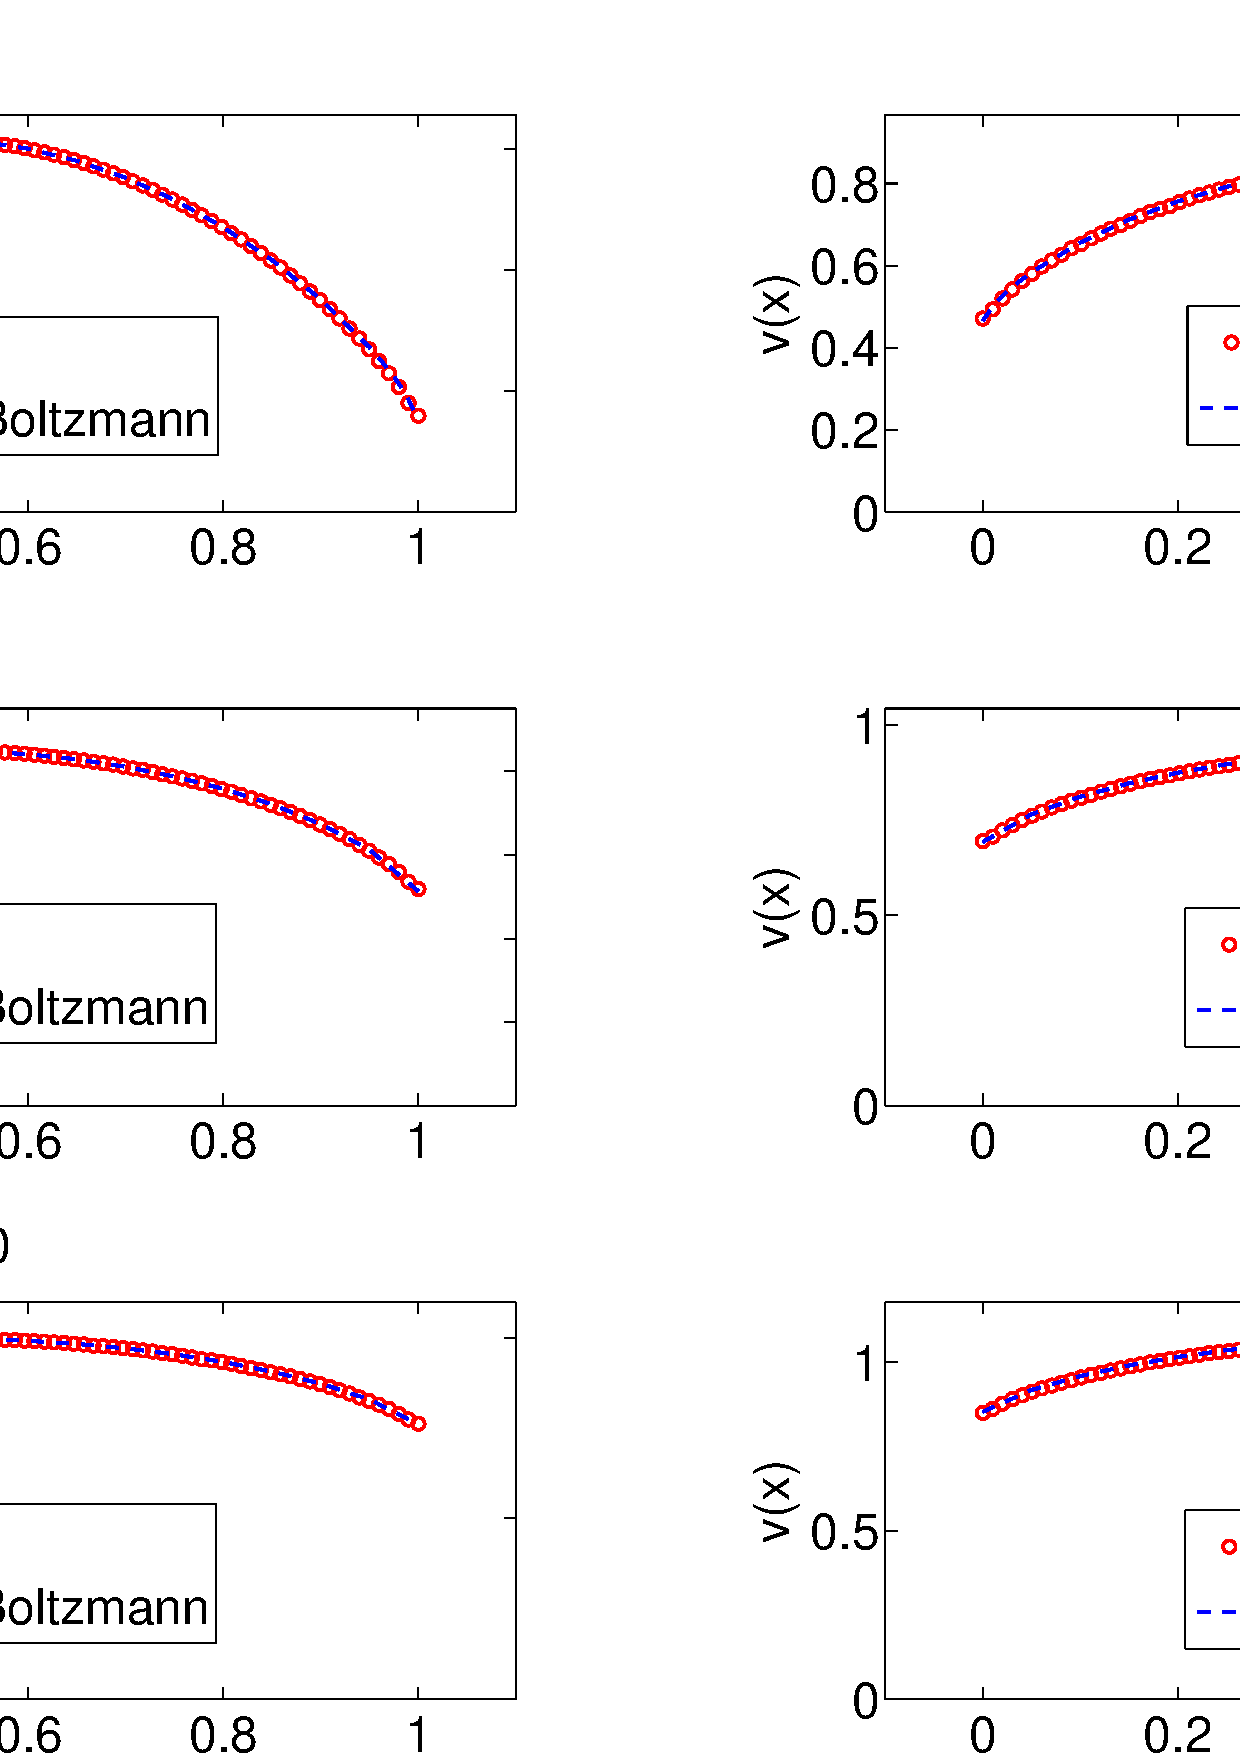
\includegraphics[scale=0.25]{figures/validation_poiseuille.pdf}
\label{fig:dsmc_validation_poiseuille}
\caption{Gravity driven Poiseuille flow}
\end{figure}

The channel is periodic in the $x-$ and $z-$direction, emulating a large system with negligible boundary effects. The gas molecules collide with the plates through the thermal wall model, so the reflected particles will have zero tangential velocity on average. In the continuum limit, $Kn\rightarrow 0$, we expect the velocity profile to approach the parabolic solution \cite{batchelor2000introduction}
\begin{align}
	v_z(y) = \nabla P\frac{1}{2\mu}y(y-h).
\end{align}
However, in the transition flow regime, $0.1 \leq Kn \leq 10$, we expect a non zero slip velocity\cite{morris1992slip}. 

The Knudsen number will affect the velocity distribution through the fact that a high Knudsen number means a larger mean free path, hence fewer inter-molecular collisions. A low collision rate will make the surface effects propagate slower through the system. We therefor expect a larger difference 

\subsubsection{Gravity driven flow}

  \section{Parallelization performance}
\label{sec:dsmc_parallelization_performance}
After the code is parallelized, the total computation time needed to perform a simulation is obviously not reduced. There are still as many collisions as before as the physical problem is identical. The idea is to do many of the calculations at the same time so that the total \textit{real} time we actually wait is reduced. Parallelizing is of course not free, as we need more logic to let the processors communicate with each other (exchanging particles and waiting for each other to finish each time step). As the number of processors increases, the total computation time \textit{per processor} is reduced, but the time spent on communication often increases. We will measure what's called \textit{parallel scalability} which indicates how efficient a program is when the number of processors is increased. There are two different kinds of scalability; weak and strong scaling
\begin{itemize}
	\item strong scaling is how the computation time changes with an increased number of processors on a fixed system size, whereas the
	\item weak scaling is how the computation time changes with an increased number of processors on a fixed system size \textit{per processor}.
\end{itemize}
\subsection{Strong scaling}
To see how the program efficiency scales with a fixed system size while increasing the number of processors is important if we want to study a specific system (a given system size and geometry, e.g. scanned from real data), but we would like to reduce the simulation run time. With a fixed system size, the total number of particles per CPU is obviously reduced while increasing the total number of processors. We define the \textit{strong scaling efficiency} $\eta_s$ as
\begin{align}
	\eta_s = \frac{t_1}{Nt_N},
\end{align}
where $t_1$ is the total run time using one processor and $t_N$ is the total run time using $N$ processors. We see that $\eta_s\in (0,1)$ since $Nt_N$ is the ideal scaling without any communication overhead. In this benchmark, we have run a geometry carved out by 10 random walkers (the algorithm is described in section \ref{sec:dsmc_random_walk_algorithm}), each starting at random positions. Each walker moves 1000 steps (voxels) with a turn probability of 0.1 on a $128\times128\times128$ voxel grid ending up with a porosity of $\phi=0.53635$. The physical system is a cube with side length $L=$\unit{1.0}{\micro\meter} with a density $\rho_n=\unit{1.0\e{25}}{\meter^{-3}}$ which gives a total of 5.3 million atoms. We choose that one DSMC particle represents one atom yielding a total of 5.3 million particles in the whole system. The benchmark was performed for 10000 timesteps ($\Delta t = 0.005$) with $2^N$ processors from 1 CPU to 512 CPUs yielding a good estimate of how efficient the program scales for a relatively large number of processors. In table \ref{tab:dsmc_strong_scaling} we have the scaling results with additional information like the number of intermolecular collisions and the number of wall collisions. These numbers indicates the amount of computation  The strong scaling efficiency is plotted against the number of processors in figure \ref{fig:dsmc_strong_scaling}.
\begin{table}
\begin{center}
    \begin{tabular}{|l|l|l|l|l|l|l}
    \hline
    $N_\text{CPU}$ & $N_\text{particles}/N_\text{CPU}$ & $N_\text{collisions}/N_\text{CPU}$ & $N_\text{wall collisions}/N_\text{CPU}$ & Run time[s] & $\eta_s$ \\ \hline
    1 & 5.4\e{6} & 1.31\e{8} & 1.09\e{11} & \unit{10571}{\second} & 1.00\\
    \hline
    2 & 2.7\e{6} & 6.55\e{7} & 5.04\e{10} &  \unit{5262}{\second} & 1.00\\
    \hline
    4 & 1.3\e{6} & 3.28\e{7} & 2.73\e{10} &  \unit{2687}{\second} & 0.984\\
    \hline
    8 & 6.7\e{5} & 1.64\e{7} & 1.36\e{10} &  \unit{1360}{\second} & 0.972\\
    \hline
    16 & 3.4\e{5} & 8.19\e{6} & 6.81\e{9} &  \unit{755}{\second} & 0.875\\
    \hline
    32 & 1.7\e{5} & 4.09\e{6} & 3.41\e{9} &  \unit{505}{\second} & 0.654\\
    \hline
    64 & 8.4\e{4} & 2.05\e{6} & 1.70\e{9} &  \unit{262}{\second} & 0.630\\
    \hline
    128 & 4.2\e{4} & 1.02\e{6} & 8.52\e{8} &  \unit{146}{\second} & 0.566\\
    \hline
    256 & 2.1\e{4} & 5.12\e{5} & 4.26\e{8} &  \unit{94}{\second} & 0.440\\
    \hline
    512 & 1.0\e{4} & 2.56\e{5} & 2.13\e{8} &  \unit{79}{\second} & 0.261\\
    \hline
    \end{tabular}
    \caption{Benchmark results showing the strong scaling efficiency $\eta_s$ for the DSMC program.}
    \label{tab:dsmc_strong_scaling}
    \end{center}
\end{table}
The reason for this scaling behavior might be due to bad load balancing since the processors might get different work load. One processor might get a subvolume that contains very few particles if most of its voxels are solid wall voxels. These processors will spend most of their time on waiting for the other processors to finish and we do not make full use of the available processors. This problem is discussed further in section \ref{sec:future_work_load_balancing}. 
\subsection{Weak scaling}
Another important scaling problem appears when we want to maximize the simulated system size. If we keep a constant system size \textit{per cpu}, and increase the number of processors, the limitation of how big we efficiently can create the system is controlled by the weak scaling. We then introduce the \textit{weak scaling efficiency} $\eta_w$ defined as
\begin{align}
	\eta_w = \frac{t_1}{t_N},
\end{align}
where again $t_1$ is the total run time using one processor and $t_N$ is the run time using $N$ processors. If the algorithm scales perfectly, the total run time would remain constant while increasing the number of processors (each CPU is ideally independent), but we expect some overhead. This implies that the range for $\eta_w$ also is between zero and one. We have run the same geometry as for the strong scaling, but each processor controls a volume of \unit{1}{\micro\meter^3} so that the largest system is \unit{512}{\micro\meter^3}. Keeping the same density gives a total of 5.3 million particles per processor. In table \ref{tab:dsmc_weak_scaling}, we see the results for the weak scaling efficiency simulation. 
\begin{table}
\begin{center}
    \begin{tabular}{|l|l|l|l|l|l|l}
    \hline
    $N_\text{CPU}$ & $N_\text{particles}$ & $N_\text{collisions}$ & $N_\text{wall collisions}$ & Run time[s] & $\eta_w$ \\ 
    \hline
    1 & 5.4\e{6} & 1.00\e{10} & 1.00\e{10} & \unit{100}{\second} & 1.0\\
    \hline
    2 & 1.27\e{6} & 1.00\e{10} & 1.00\e{10} & \unit{100}{\second} & 1.0\\
    \hline
    4 & 1.27\e{6} & 1.00\e{10} & 1.00\e{10} & \unit{100}{\second} & 1.0\\
    \hline
    8 & 1.27\e{6} & 1.00\e{10} & 1.00\e{10} & \unit{100}{\second} & 1.0\\
    \hline
    16 & 1.27\e{6} & 1.00\e{10} & 1.00\e{10} & \unit{100}{\second} & 1.0\\
    \hline
    32 & 1.27\e{6} & 1.00\e{10} & 1.00\e{10} & \unit{100}{\second} & 1.0\\
    \hline
    64 & 1.27\e{6} & 1.00\e{10} & 1.00\e{10} & \unit{100}{\second} & 1.0\\
    \hline
    128 & 6.87\e{8} & 1.67\e{10} & 5.86\e{11} & \unit{12032}{\second} & 1.0\\
    \hline
    256 & 1.37\e{9} & 3.33\e{10} & 1.05\e{12} & \unit{16418}{\second} & 1.0\\
    \hline
    512 & 2.75\e{9} & 6.59\e{10} & 1.87\e{12} & \unit{18242}{\second} & 1.0\\
    \hline
    \end{tabular}
    \caption{Benchmark results showing the weak scaling efficiency $\eta_w$ for the DSMC program.}
    \label{tab:dsmc_weak_scaling}
    \end{center}
\end{table}

\begin{figure}[h]
\begin{center}
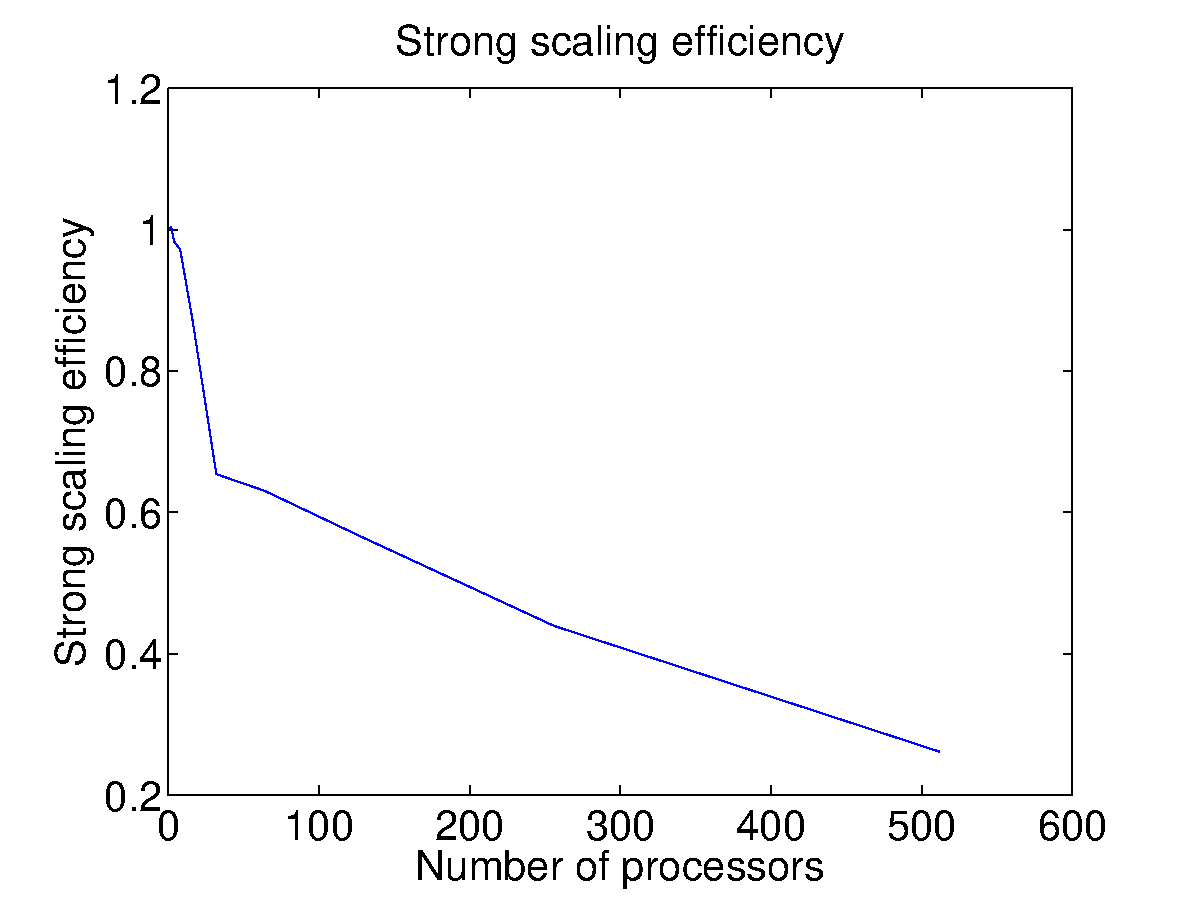
\includegraphics[width=\textwidth, trim=0cm 0cm 0cm 0cm, clip]{DSMC/figures/strong_scaling.eps}
\end{center}
\caption{The weak and strong scaling efficiency, $\eta_w$ and $\eta_s$, as a funtion of the number of processors $N_\text{CPU}$. We see that at 512 processors, the efficiency is reduced to 25\% because of the large overhead from the MPI communication.}
\label{fig:dsmc_strong_scaling}
\end{figure}
\section{Results for simple geometries}
\label{sec:results_for_simple_geometries}
In this section, we will study flow in simple geometries where the theoretical permeability is well known. The expression for the permeability is only valid for small Knudsen numbers (which we called the absolute permeability; the permeability for fluids in the continuum limit), so it is a perfect test case for the Knudsen correction factor $f_c$ in equation \eqref{eq:knudsen_correction}. 

\subsection{Flow in a cylinder, varying Knudsen number}
We have induced flow in a cylinder with radius \unit{0.45}{\micro\meter} with an applied acceleration corresponding to a pressure difference $\Delta P = 1.1P_0$, where $P_0$ is the ideal gas pressure at \unit{300}{\kelvin}. We want to vary the Knudsen number which was defined as
\begin{align}
	\text{Kn} = \frac{\lambda}{L} = \frac{1}{\sqrt 2 \pi d^2 \rho_n L}
\end{align}
where $L$ is the length of the cylinder, $\lambda$ is the mean free path. We have used equation \eqref{eq:mean_free_path} in the last expression so that we can choose the Knudsen number through the density
\begin{align}
	\rho_n(\text{Kn}) = \frac{1}{\sqrt 2 \pi d^2 \text{Kn}L}.
\end{align}
We expect an apparent permeability satisfying the Knudsen correction
\begin{align}
	k_a = k_\infty f_c = k_\infty[1 + \alpha(\text{Kn})\text{Kn}]\left[1 + {4\text{Kn}\over 1 + \text{Kn}}\right].
\end{align}
The analytical absolute permeability for a cylinder with radius $r$ is given by\cite{karniadakis2005microflows}
\begin{align}
	\label{eq:permeability_cylinder}
	k_\infty = {r^2\over 8},
\end{align}
which gives the following prediction for the apparent permeability
\begin{align}
	k_a = [1 + \alpha(\text{Kn})\text{Kn}]\left[1 + {4\text{Kn}\over 1 + \text{Kn}}\right] {r^2\over 8}.
\end{align}
In figure \ref{fig:one_cylinder_varying_knudsen} we have plotted the measured permeability as a function of Knudsen number. We see that the 

\begin{figure}[h]
\begin{center}
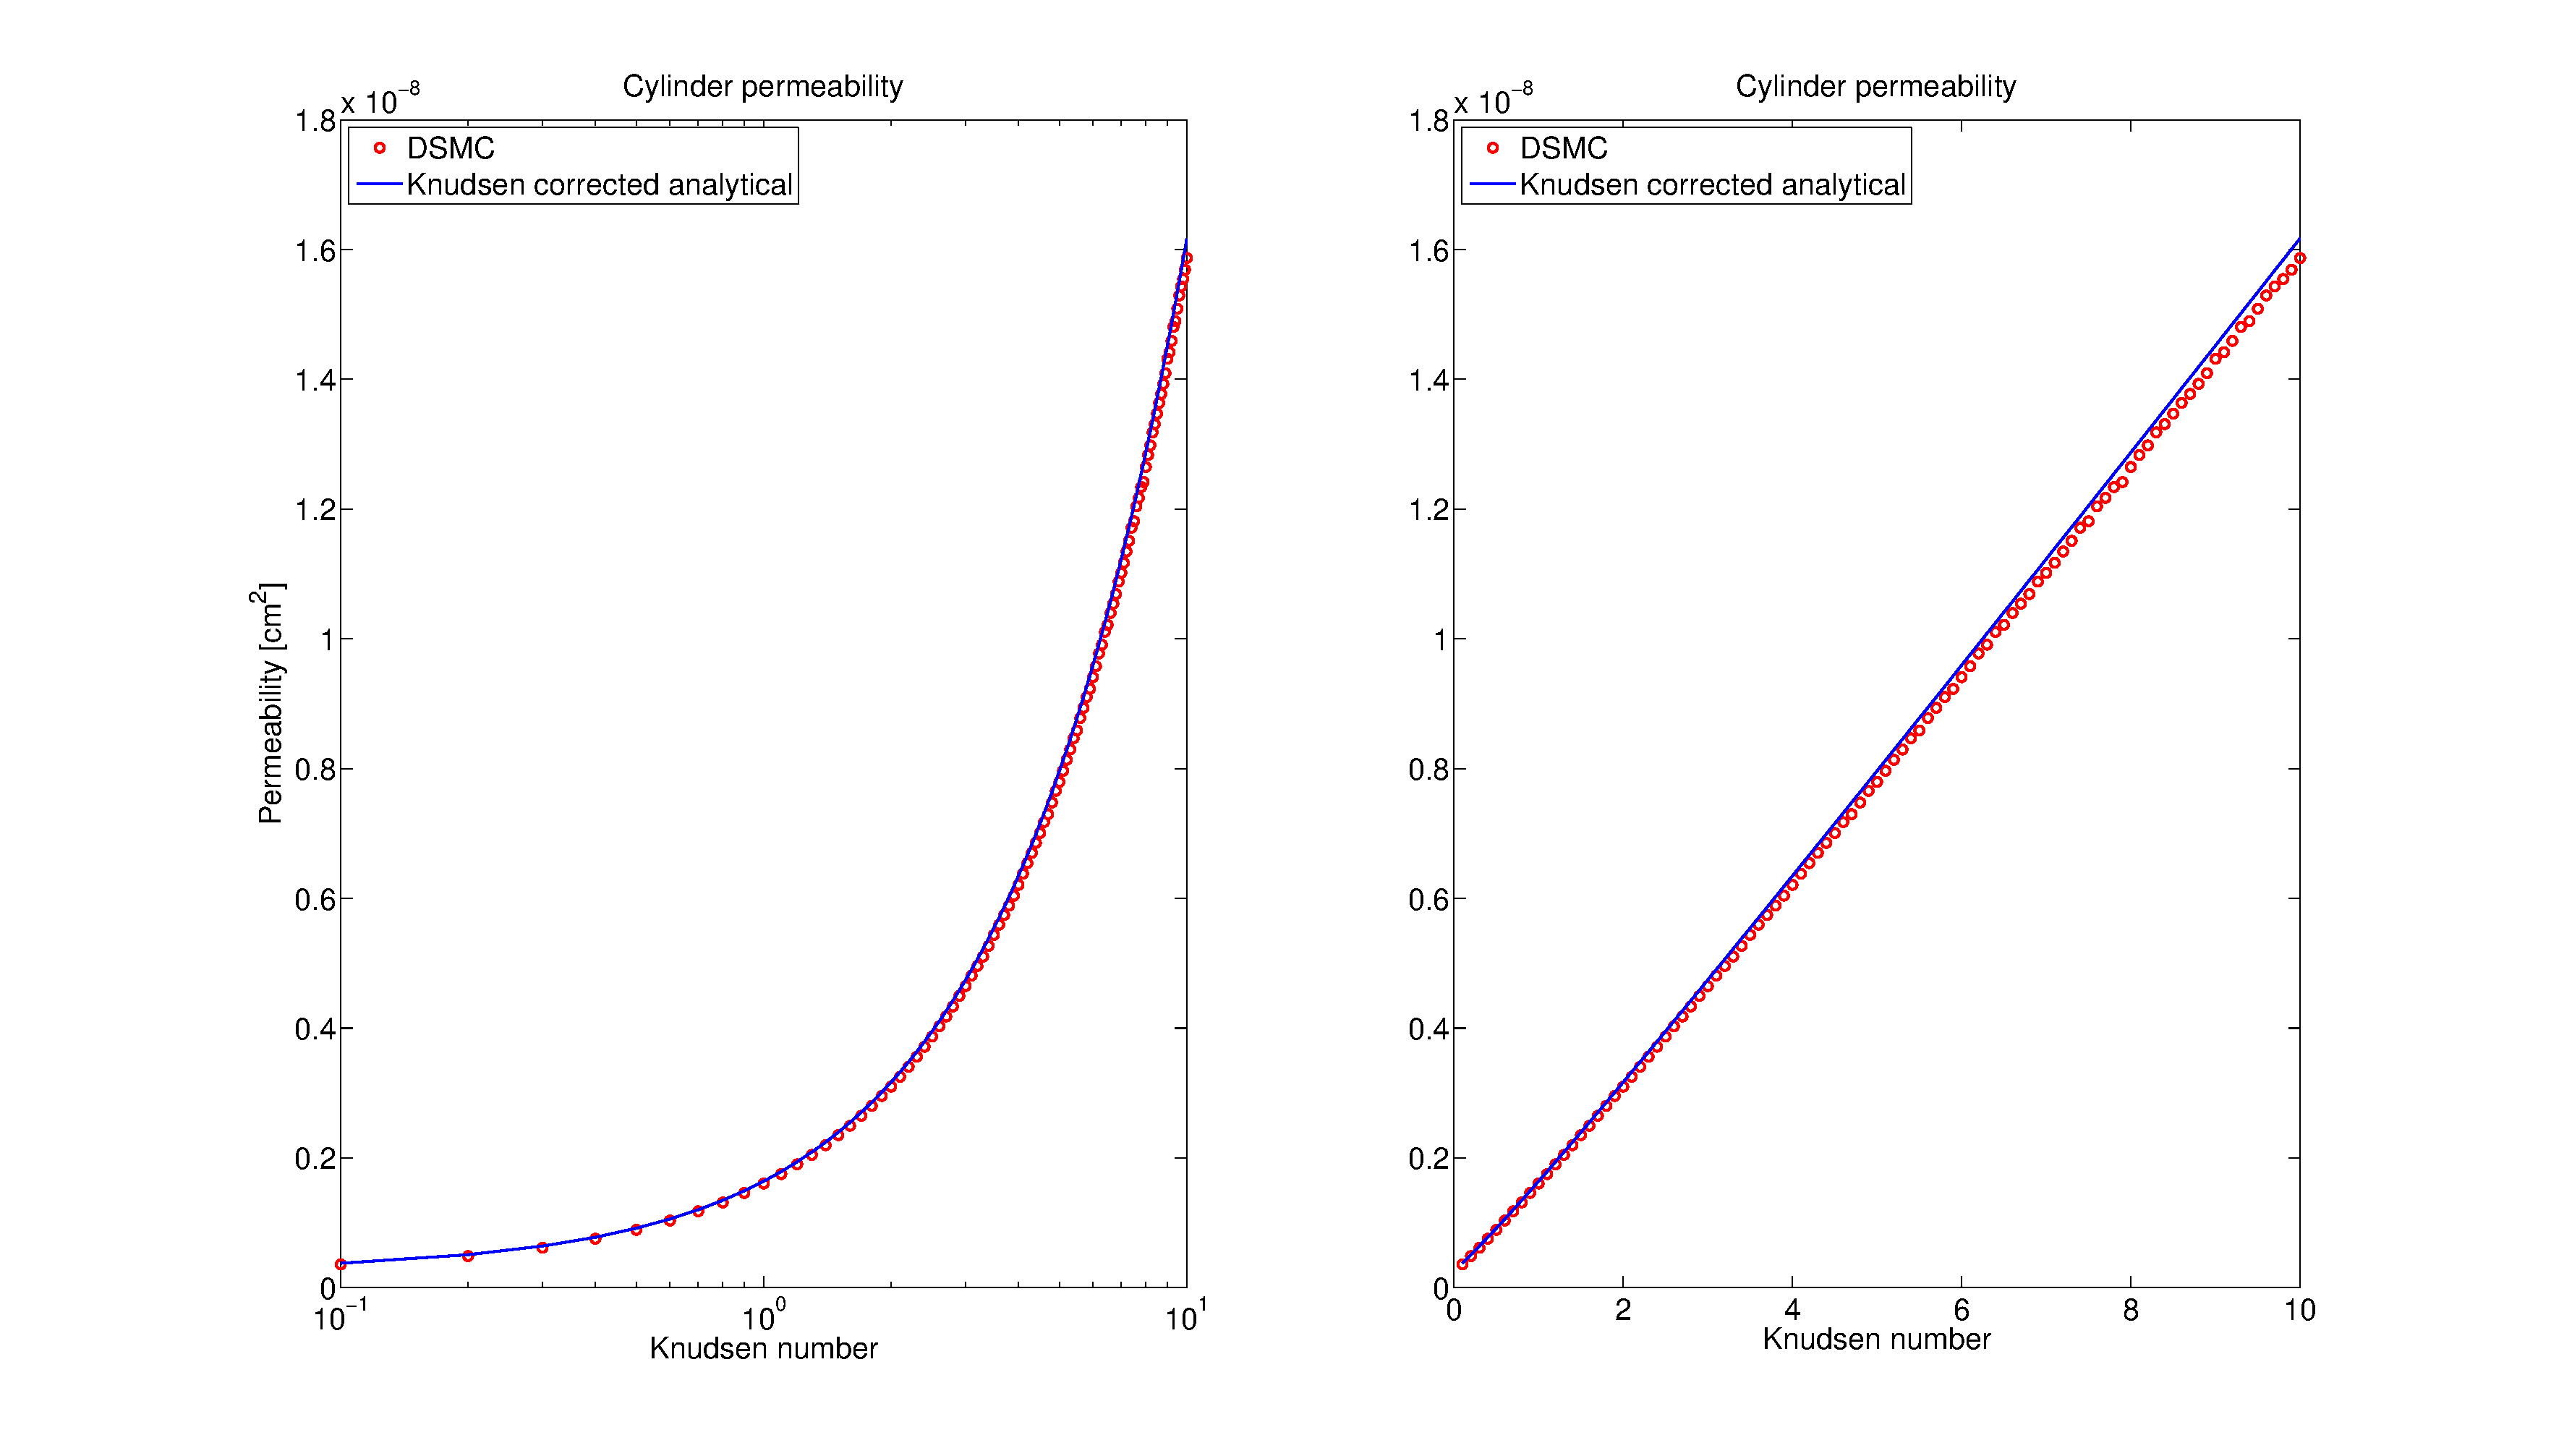
\includegraphics[width=\textwidth, trim=0cm 0cm 0cm 0cm, clip]{DSMC/figures/cylinder_knudsen_permeability.eps}
\end{center}
\caption{Permeability as a function of Knudsen number for a cylinder with radius \unit{0.45}{\micro\meter} and length \unit{1}{\micro\meter} with an applied pressure difference $\Delta P = 1.1P_0$ ($P_0$ being the ideal gas pressure). We control the Knudsen number by varying the density. The blue line is the Knudsen corrected analytical solution from \cite{karniadakis2005microflows}. The DSMC results confirm that the Knudsen correction factor works very well for a system with a well defined Knudsen number.}
\label{fig:one_cylinder_varying_knudsen}
\end{figure}

\subsection{Flow in a cylinder, varying radius}
If we instead keep the Knudsen number constant ($\text{Kn}=1.0$), we can vary the radius to verify equation \eqref{eq:permeability_cylinder}. We have studied radii in the range \unit{0.1}{\micro\meter} to \unit{0.45}{\micro\meter} with the same pressure difference as in the previous simulation ($\Delta P = 1.1P_0)$. In figure \ref{fig:one_cylinder_varying_radii_result} we have plotted the measured permeability as a function of cylinder radius. The straight line confirms the quadratic dependency in equation \eqref{eq:permeability_cylinder}.
\begin{figure}[h]
\begin{center}
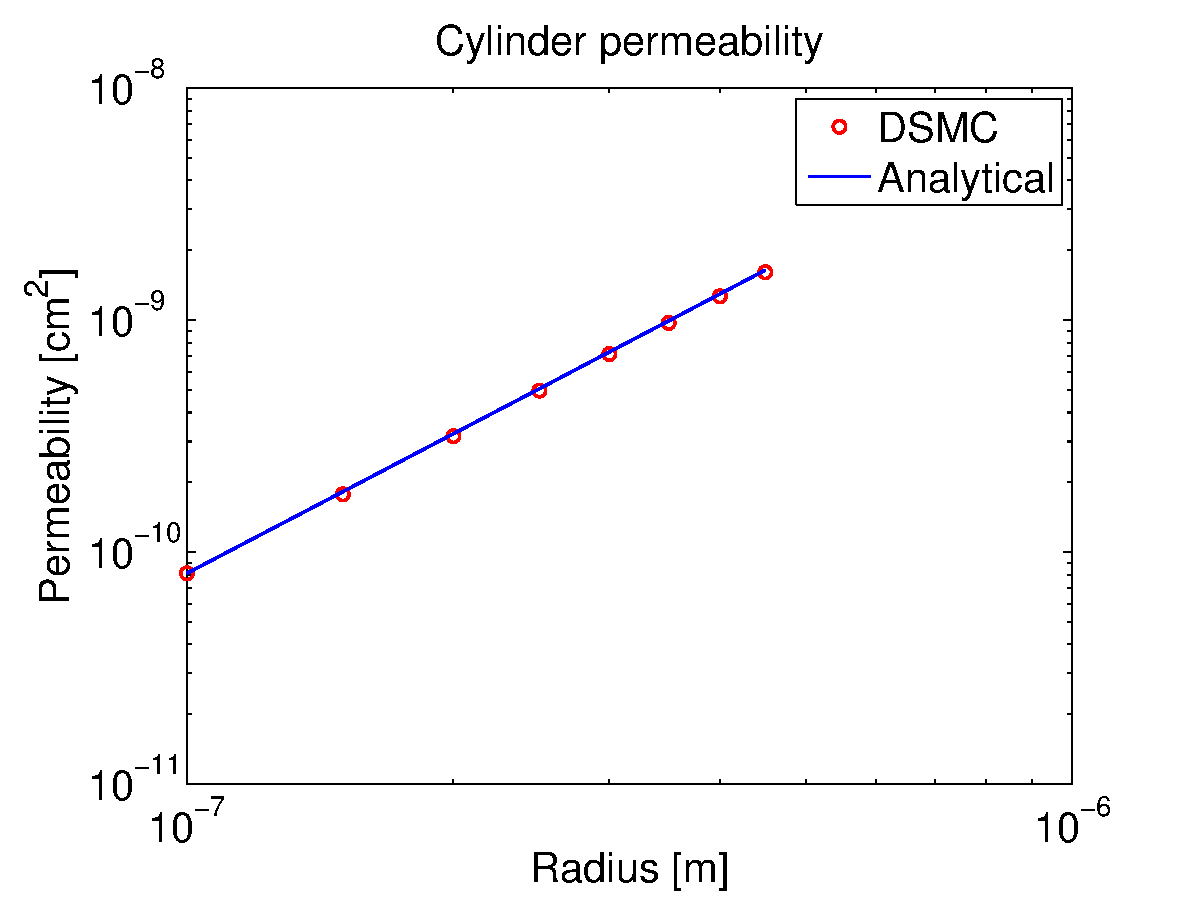
\includegraphics[width=\textwidth, trim=0cm 0cm 0cm 0cm, clip]{DSMC/figures/cylinder_radius_permeability.eps}
\end{center}
\caption{Logarithmic plot of the permeability for different cylinders with radii in the range $0.1 \mu m$ to $0.45 \mu m$ with an applied pressure difference $\Delta P = 1.1P_0$. The blue line is the Knudsen corrected analytical solution from \cite{karniadakis2005microflows}.}
\label{fig:one_cylinder_varying_radii_result}
\end{figure}
\section{Results for complicated geometries}
We have now seen that the Knudsen correction factor works well for systems with a well defined Knudsen number. The Knudsen correction factor needs an exact Knudsen number to be able to predict the permeability, but for more complex geometries, there is rather a distribution of Knudsen numbers than a single number. It could work as a lower and an upper limit of the permeabilities for two different input Knudsen numbers, but they could differ by an order of magnitude. In this section we will study a system consisting of randomly packed spheres that does not have a well defined Knudsen number.
\subsection{The Carman-Kozeny equation}
In 1927, Kozensky proposed an equation predicting the permeability of packed spheres of radius $a$ forming a system with porosity $\phi$ given as
\begin{align}
	k = {a^2 \over 9K} {\phi^3 \over (1 - \phi)^2},
\end{align}
where $K$ is the Kozeny constant which is experimentally measured to be around five\cite{carman1937fluid}. This result has been verified to predict permeabilities in many experiments since its discovery. However, at the nanometer scale, we expect deviations due to high Knudsen numbers. 
\subsection{The simulation}

\end{chapter}
\end{part}

\begin{part}{Molecular Dynamics}
  \label{chap:md}
  \begin{chapter}{Introduction}
  Molecular Dynamics is another numerical model that describes the behaviour of liquids, gases and solids at the finest scale of any classical model. We can study the dynamics of single atoms and how they interact with each other forming molecules and larger objects like advanced pore networks. The idea is simple and has been used since the time of Sir Isaac Newton in the 17th century when he formulated his laws of motion. With the knowledge of the relevant forces between the atoms, we can solve Newton's equations and calculate their dynamics.

We open this chapter by a short introduction to the model in section \ref{sec:md_model} before we explain how forces are calculated with the Lennard-Jones potential in section \ref{sec:md_forces}. With computed forces, we can integrate the atoms with Newton's laws following an time integration scheme which we discuss in section \ref{sec:md_time_integration}. The last section is concerned with how we measure physical quantities which will be very similar to what we did with DSMC in section \ref{sec:dsmc_measuring_physical_quantities}.
  \section{The model}
\label{sec:md_model}
The state of a Molecular Dynamics system is fully described by seven variables per atom; three positions, three velocities plus the atom type. The phase variables are evolved through the laws of motion. It is here common, as in DSMC (see section \ref{sec:dsmc_model}), to apply periodic boundary conditions. Applied periodic boundary conditions in all directions implies constant volume (unless, of course, we rescale the system size which can be done). The atomic forces are calculated as the gradient of a chosen potential that can differ quite a lot depending on the requirements of the model. A noble gas like Argon can be modeled with a simple potential called the Lennard-Jones potential which will be discussed below. With this potential, one can calculate equilibrium thermodynamic properties that are in good agreement with experimental values \cite{verlet1967computer}. System statistics are sampled as ensemble averages through ergodicity over large times. A typical Molecular Dynamics algorithm is illustrated in figure \ref{fig:flow_simple_md}.
\begin{figure}[h]
\framebox{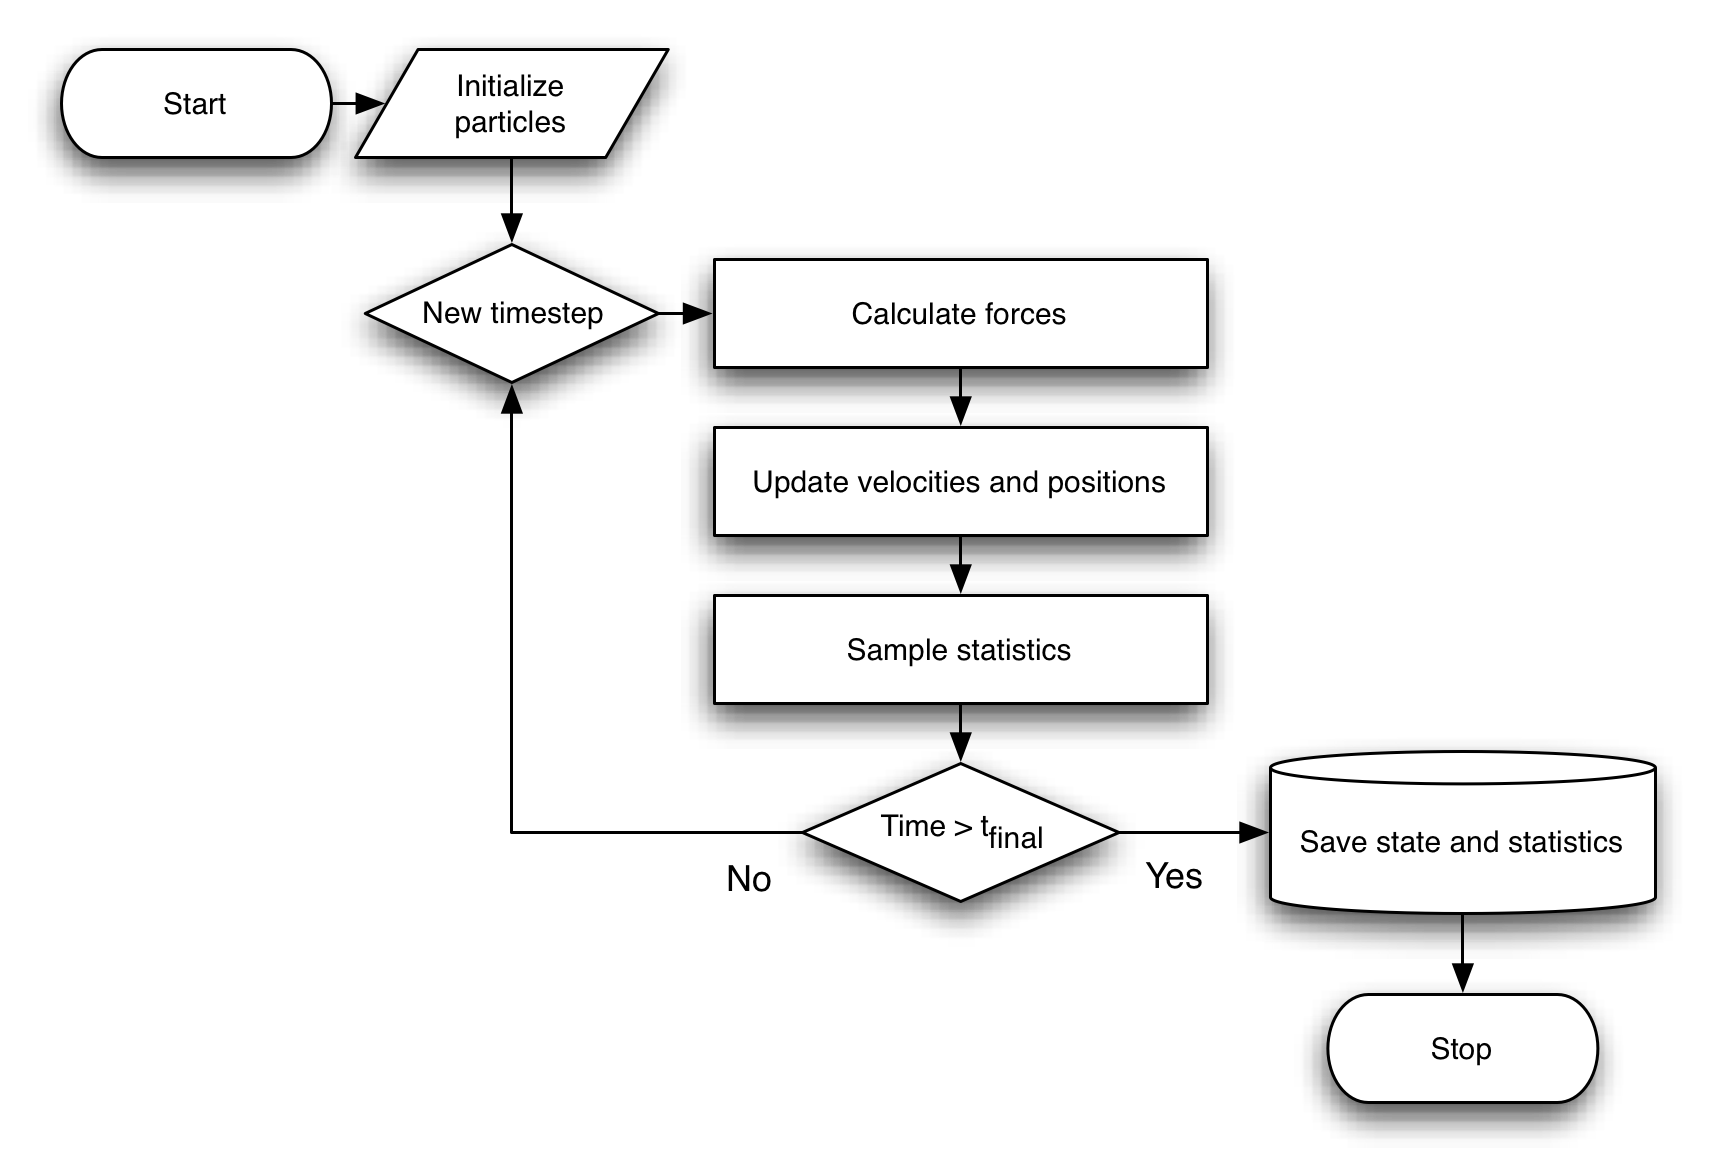
\includegraphics[width=0.8\textwidth, trim=0cm 0cm 0cm 0cm, clip]{MD/figures/SimpleMD.png}}
\centering
\caption{Flow chart illustrating a typical Molecular Dynamics algorithm.}
\label{fig:flow_simple_md}
\end{figure}
  \section{Physical properties}
The phase space variables can be used to sample statistical properties of the system. Properties of interest are kinetic and potential energy, temperature, pressure, diffusion constant and different correlation functions (such as the pair correlation function, cage-correlation function, static and the dynamic structure factor). In this section, we will define these properties and discuss how to measure them.
\subsection{Kinetic and potential energy}
We measure the kinetic energy directly through its definition for point particles
\begin{align}
	E_k = \sum_i \frac{1}{2} m_iv_i^2,
\end{align}
where $m_i$ is the mass of particle $i$ and $v_i$ is the velocity of the particle. The potential energy is measured by evaluating \eqref{eq:md_potential_energy}. We define temperature by applying the equipartition theorem using the momentum degrees of freedom
\begin{align*}
	E_k = \frac{f}{2}kT,
\end{align*}
where $f=3N$ are the three momentum variables per particle, $T$ is the temperature and $k$ is Boltzmann's constant. Solving the equation for the temperature yields
\begin{align}
	T = \frac{2E_k}{3Nk},
\end{align}
which is how we \textit{define} temperature in this model. 
\subsection{Pressure}
We will derive an expression for the pressure by using Clausius' virial function
\begin{align}
    W(\textbf{r}) = \sum_{i=1}^N \vec r_i \cdot \vec F_i^{TOT},
\end{align}
where $F_i^{TOT}$ is the total force acting on atom $i$, including external forces. We assume equilibrium, so that the kinetic energy has reached an approximately constant value. We measure the statistical average of $W$ by calculating
\begin{align}
    \langle W \rangle &= \lim_{t\rightarrow\infty} {1\over t} \int_0^t d\tau \sum_{i=1}^N \vec r_i(\tau) \cdot m_i \vec{\ddot r}_i(\tau).
\end{align}
Integrating by parts gives
\begin{align}
    \label{eq:virial_and_equi}
    \langle W \rangle &= -\lim_{t\rightarrow\infty} {1\over t} \int_0^t d\tau \sum_{i=1}^N m_i |\vec{\dot r}_i(\tau)|^2 = -2E_k = -3Nk_bT,
\end{align}
by again using equipartition. Now, assume that the atoms live inside a parallelepipedic container of size $L_x, L_y, Lz$ with hard walls, with origo in one of its corners. If we divide the force into external and interatomic forces, $\vec F_i^{TOT} = \vec F_i + \vec F_i^{EXT}$, and assume that the external forces are forces from the container (no gravity or electric fields), we can calculate $W^{EXT}$. The atoms near the walls apply a pressure on the wall $P = F/A$. As an example, we look at all the atoms that are near the wall located at $x=L_x$. The virial function gives
\begin{align}
    W^{EXT}_x = \sum_{n=1}^{N_x}\vec r_n\cdot \vec F_n^{EXT},
\end{align}
where $n$ now sums over all atoms that are near the container wall at $x=L_x$. The position vectors are $\vec r_n = (L_x, y_n, z_n)$ and the force only has a component normal to the wall $F_n^{EXT} = 1/N_x(-PL_yL_z, 0, 0)$. We then get
\begin{align}
    W^{EXT}_x = -L_xPL_yL_z = -PV,
\end{align}
and by doing the same for the other dimensions, we get
\begin{align}
    W = -3PV.
\end{align}
Inserting this result into \eqref{eq:virial_and_equi} yields
\begin{align}
    \left\langle \sum_{i=1}^N \vec r_i \cdot \vec F_i\right\rangle - 3PV = -3Nk_bT
\end{align}
which can be rearranged to
\begin{align}
    PV = Nk_bT - \frac{1}{3}\left\langle \sum_{i=1}^N \vec r_i \cdot \vec F_i\right\rangle.
\end{align}
Using this result, we can define the pressure
\begin{align}
	P = \rho k_bT - \frac{1}{3V}\left\langle \sum_{i=1}^N \vec r_i \cdot \vec F_i\right\rangle,
\end{align}
where $\rho$ is the density.
\subsection{Radial distribution function $g(r)$}
The thermodynamic properties like temperature, pressure and volume give little or no information about the microscopic structure of the system. If the atoms forms a solid and are organized in some sort of a crystal (see figure \ref{fig:crystal}), one could be interested in measuring what kind of crystal they form. Different structures and symmetries of the crystal give rise to different physical properties like electronic band structure, optical transparency among others\cite{kittel1996introduction}. The crystal structure can be studied through what is called the radial distribution function, $g(r)$, which is a function proportional to the probability of finding an atom at a distance $r$ from another atom. A non-perfect FCC lattice (non-perfect in the sense that the atoms are vibrating around the equilibrium) will have a $g(r)$ as in figure \ref{fig:fcc_lattice_g_of_r}.\\
\begin{figure}[h]
\framebox{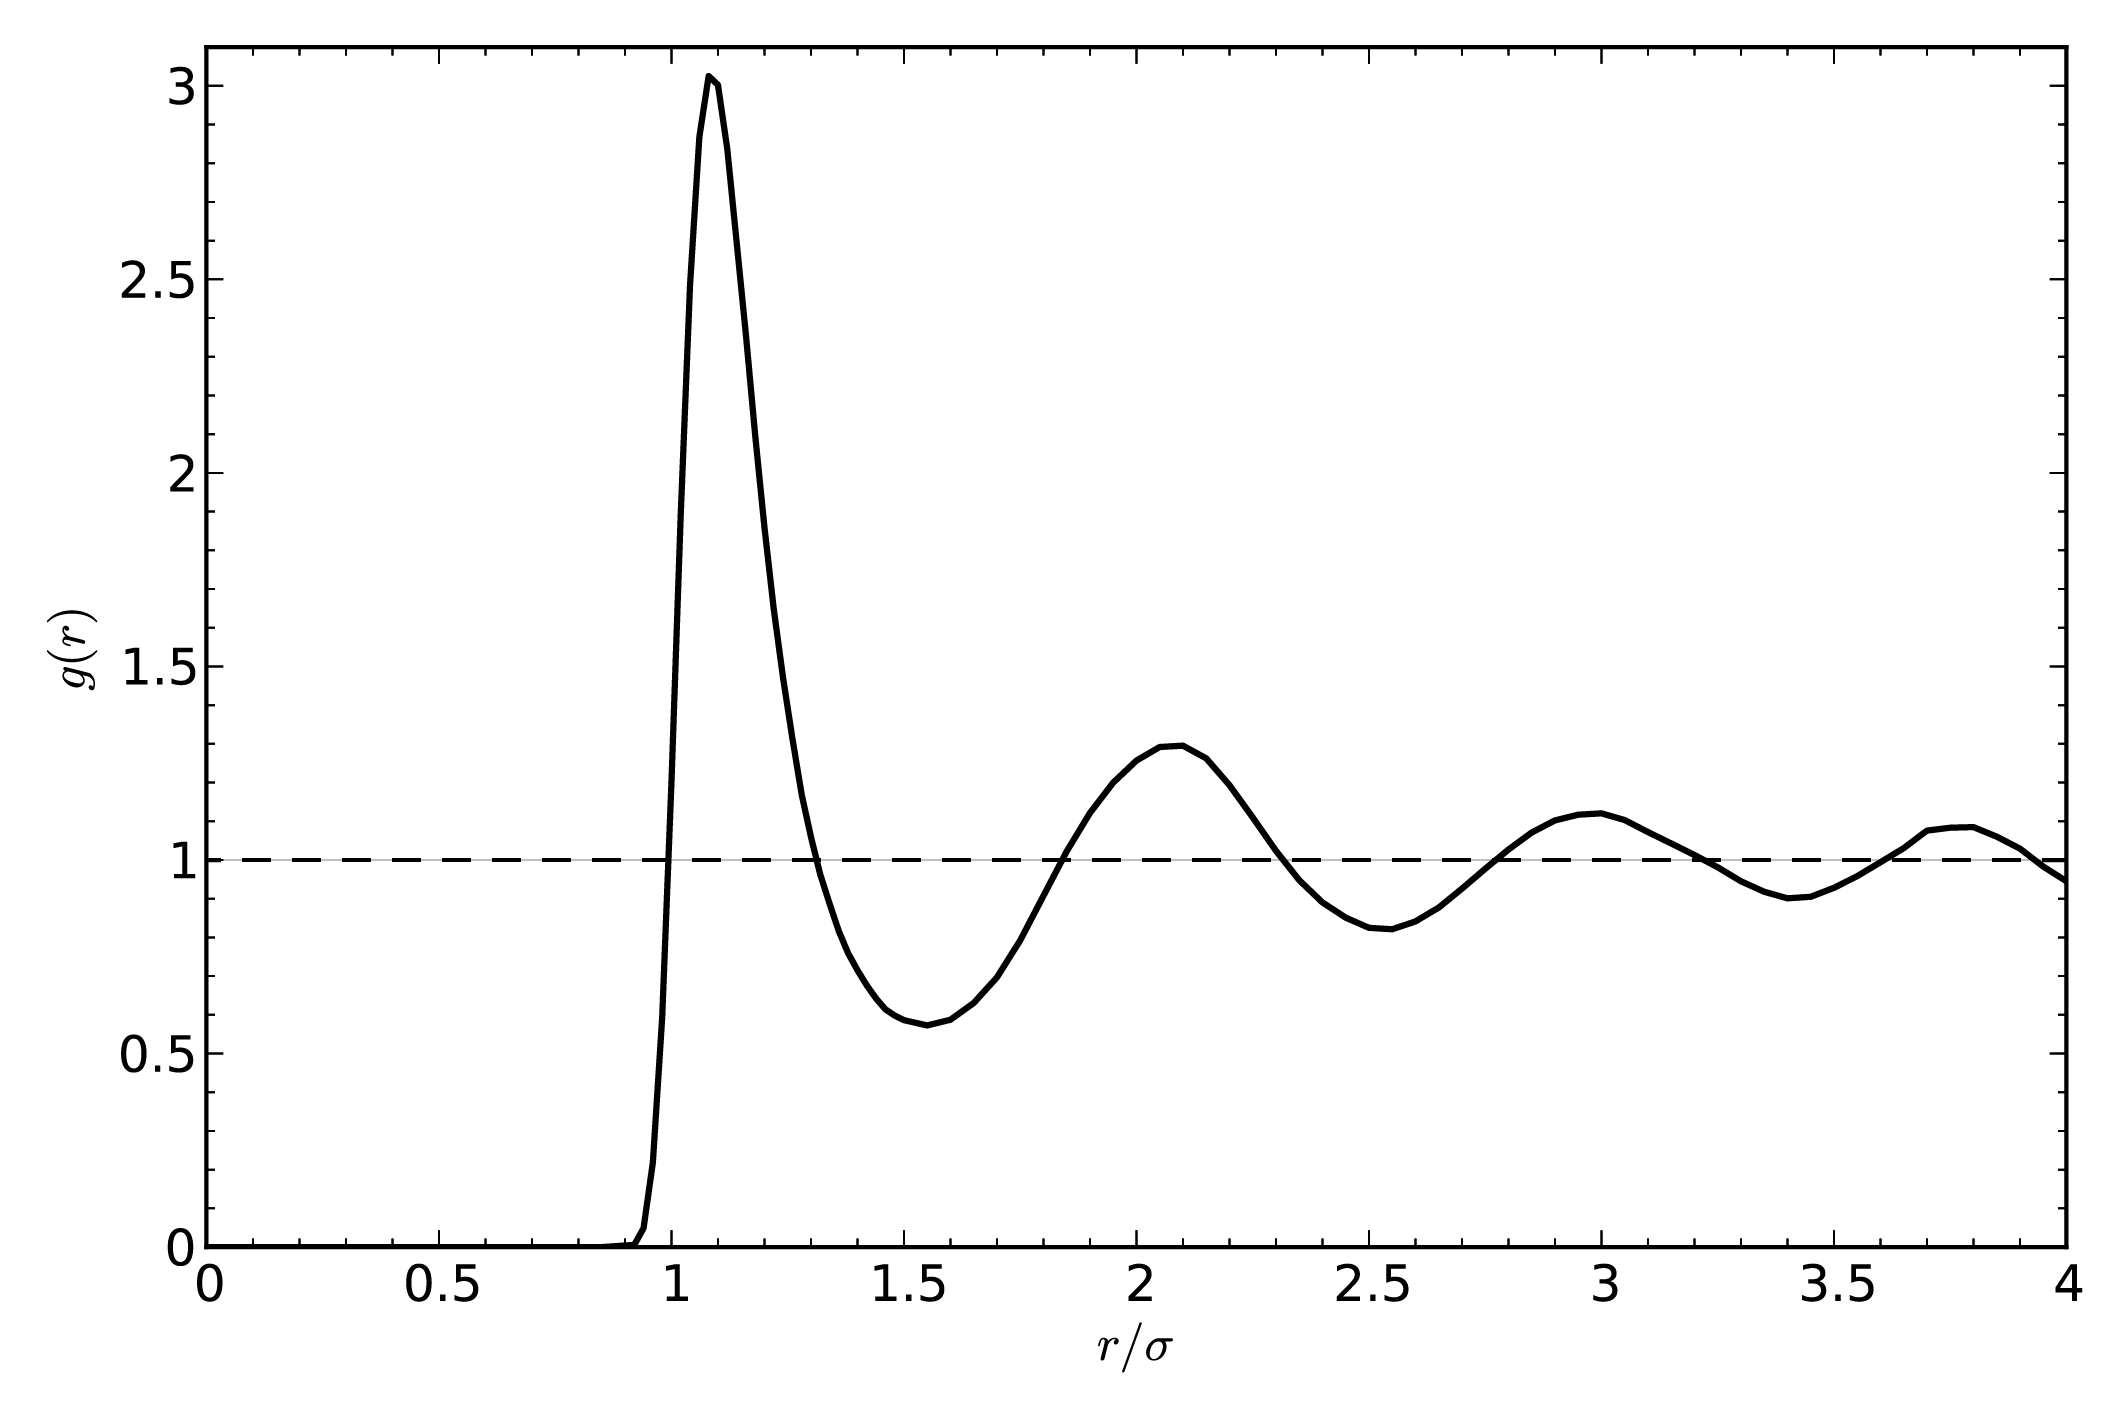
\includegraphics[width=\textwidth, trim=0cm 0cm 0cm 0cm, clip]{MD/figures/lennardjonesg_of_r.png}}
\label{fig:fcc_lattice_g_of_r}
\centering
\caption{The radial distribution function of an FCC lattice. The first peak reveals the distance between the face atoms and the corner atoms. Source: \url{http://en.wikipedia.org/wiki/Radial_distribution_function}.}
\end{figure}
The radial distribution function is defined as
\begin{align}
    \label{eq:g_of_r}
    g(r)dr &= \left\langle \sum_{i\neq j}\delta(r - |\vec r_i - \vec r_j|)\right\rangle{V\over N(N-1)4\pi r^2}\\
    &= {1 \over N} \left\langle \sum_{i\neq j}\delta(r - |\vec r_i - \vec r_j|)\right\rangle
\end{align}
where $N$ is seen as a normalization factor making sure that $\lim r\rightarrow \infty = 1$. A numerical implementation would loop over all relevant atom pairs, calculate their relative distance $r_{ij}$ and create a histogram over such distances. We would have to normalize each histogram bin by the volume of spherical shell as in \eqref{eq:g_of_r} with $dr\rightarrow \Delta r$ since each bin has a radial thickness. An implementation in $c++$ is given in  listing \ref{lst:g_of_r}.

\begin{lstlisting}[caption=Calculation of $g(r)$., label=lst:g_of_r]
vector<double> calculate_g_of_r(System &system, int num_bins) {
    // Create empty array of num_bins bins to store g(r)
    vector<double> g_of_r(num_bins,0);
    int num_atoms = system.r.size();

    // Loop over all atom pairs and put their distance into bin
    for(int i=0; i<num_atoms-1; i++) {
        Vector3D &r1 = system.r[i];
        for(int j=i+1; j<num_atoms; j++) {
            Vector3D &r2 = system.r[j];
            double dr = (r1 - r2).length();
            int bin_index = (dr / r_max) * num_bins;
            g_of_r[bin_index]++;
        }
    }

    // Normalize each bin
    for(int bin_index=0; bin_index<num_bins; bin_index++) {
        double r_inner = r_max * double(bin_index) / num_bins;
        double r_outer = r_max * double(bin_index+1) / num_bins;
        double r = 0.5*(r_inner + r_outer);
        double dr = r_outer - r_inner;

        double shell_volume = 4*M_PI*pow(r,2.0)*dr;
        double density = num_atoms/system.volume;
        g_of_r[bin_index] /= shell_volume * (num_atoms-1) * density;
    }

    return g_of_r;
}
\end{lstlisting}
The example code has complexity $N^2/2$, but since $g(r)$ is interesting only for relatively small $r$, we can improve the algorithm substantially by creating neighbor lists for each atom before looping over all relevant pairs. Experimentally, it is possible to measure the radial distribution function through diffraction experiments. By firing a beam of electrons or neutrons at the crystal, the electrons will be diffracted in different directions depending on the crystallic structure. One can measure the angles and intensities of the diffracted beams and then measure what is called \textit{structure factor} given by
\begin{align}
    S(\vec q) = {1\over N}\left\langle \sum_{jk} e^{-i\vec q(\vec R_j - \vec R_i)}\right \rangle,
\end{align}
where $\vec q$ is the spatial frequency (reciprocal coordinate), $N$ the number of atoms and $\vec R_{ij}$ the position of particles $i$ and $j$ respectively. We will not go into more detail in what the structure factor is other than that it is related to $g(r)$ through
\begin{align}
    S(q) = 1 + 4\pi\rho\frac{1}{q}\int dr r\sin(qr)[g(r) - 1],
\end{align}
if we assume that the material is isotropic\cite{kittel1996introduction}. The $g(r)$ can then be found through the inverse fourier transform
\begin{align}
    g(r) = 1 + {1\over 2\pi^2\rho r} \int dq(S(q) - 1)q\sin(qr).
\end{align}

\section{Diffusion constant}
The diffusion constant $D$ is defined by using the Einstein relation
\begin{align}
    \langle \Delta r^2 \rangle = 2dDt,
\end{align}
where $t$ is time, $d$ is the number of spatial dimensions and $\langle \Delta r^2 \rangle$ is average square displacement 
\begin{align}
    \langle \Delta r^2 \rangle = {1 \over N} \sum_{n=1}^N |\vec r(t) - \vec r(0)|^2.
\end{align}
In three dimensions, the diffusion constant is then found as
\begin{align}
    D = {\langle \Delta r^2 \rangle\over 6t}.
\end{align}
This is a fairly simple calculation, but in the MD-simulation, we need to keep track of how far each atom has moved from its initial position. A simple implementation is given in listing \ref{lst:diffusion}.
\begin{lstlisting}[caption=Calculation of the diffusion constant., label=lst:diffusion]
double calculate_diffusion_constant(System &system) {
    double rSquared = 0;
    for(int atom_index=0; atom_index<system.num_atoms; atom_index++) {
        double dr2 = (system.r[atom_index] - system.r0[atom_index]).length_squared();
        rSquared += dr2;
    }
    rSquared /= system.num_atoms; // Normalize to get <r^2>
    double diffusion_constant = rSquared / (6*system.t);
    return diffusion_constant;
}
\end{lstlisting}

  \section{Numerical stability}
\subsection{Tail correction}
  \section{Reaching a steady state}

  \section{Computational cost}
\label{sec:computationalcost}
  \end{chapter}

  \begin{chapter}{Implementation}
    \section{Implementation}

\subsection{Periodic boundary conditions}

\subsection{Two-body forces}
\label{sec:md_implementation_two_body_forces}
The Lennard-Jones potential gives rise to a two-body force acting only on pairs of atoms. In principle, this means we have to sum over all pairs in the system which for $n$ atoms in the system is $O(n^2)$. This calculation can be reduced to $O(n)$ by realizing that the gradient of the potential (hence the force) is nearly zero at $r \approx 2.5\sigma$, see figure \ref{fig:md_lennard_jones_2}. \todo{Show lennard jones force instead}
\begin{figure}[h]
\begin{center}
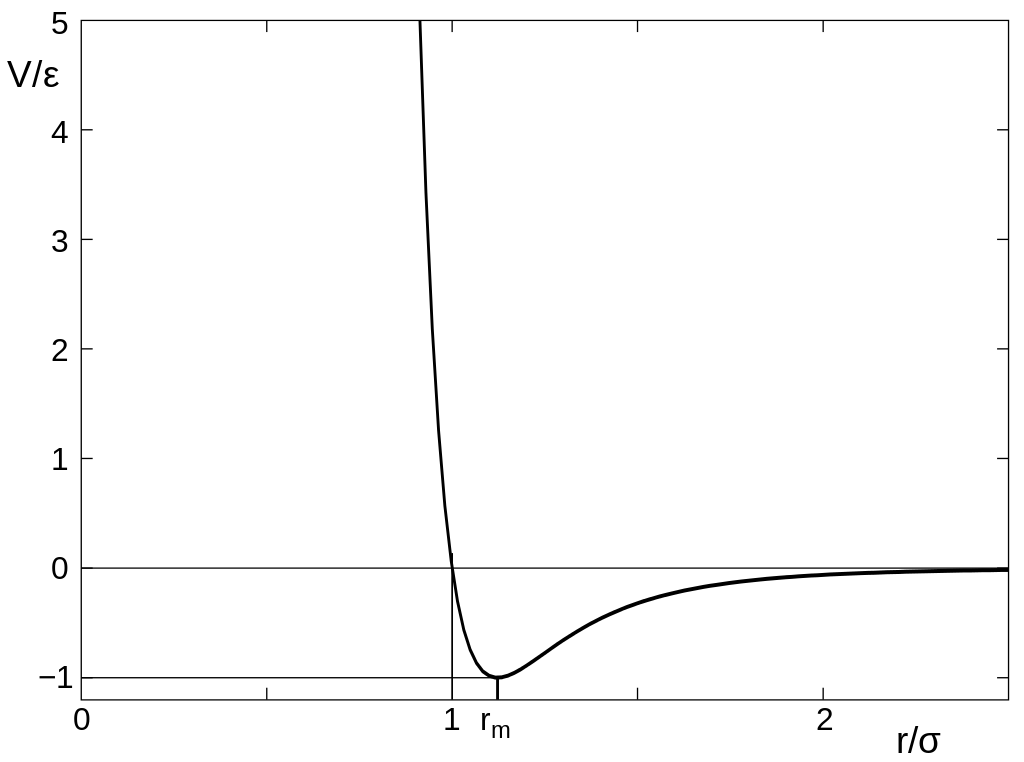
\includegraphics[width=1.0\textwidth, trim=0cm 0cm 0cm 0cm, clip]{MD/figures/lennard_jones.png}
\end{center}
\caption{The Lennard-Jones force. We see that the force is nearly zero at $r\approx 2.5\sigma$, so we don't need to calculate forces between atoms separated by a distance larger than $r_\text{cut} \equiv 2.5\sigma$.}
\label{fig:md_lennard_jones_2}
\end{figure}
We now introduce a certain cut-off distance $r_{cut}$ which we choose as the distance where the force is nearly zero, and set the force to be zero for any $r>r_{cut}$. The force between a pair of atoms $F(r_{ij})$ is then written as
\begin{align}
	F(r_{ij}) = \left\{\begin{array}{cc}
		F_{LJ}(r_{ij}) & \text{if } r \leq r_{cut}\\
		0 & \text{if } r > r_{cut}.
	\end{array}
	\right.
\end{align}
where $F_{LJ}$ is the standard Lennard-Jones force from eq \eqref{eq:md_lj_force}. We now don't need to sum over atom pairs of which the relative distance is larger than $r_cut$, so the calculation of forces is then globally $O(N)$. 
    \section{Parallelization}
\label{sec:md_parallelization}
Da parallelization technique is straight-up similar ta what tha fuck our phat asses did up in DSMC up in section \ref{sec:dmsc_parallelization}. Da spatial domain is divided tha fuck into $P_x\times P_y\times P_z$ smalla domains ($P_i$ bein tha number of processors up in tha $i$th dimension). Each such domain is then of size $l_x\times l_y \times l_z$ where $l_i = L_i/P_i$. Da processor arrangement n' labelin is done as shown up in figure \ref{fig:md_parallelization_2}, where a processor wit coordinates $(p_x, p_y, p_z)$ controls atoms wit coordinates up in tha range
\begin{align}
	\nonumber
	x&\in[p_xl_x, (p_x+1)l_x\rangle\\
	\nonumber
	y&\in[p_yl_y, (p_y+1)l_y\rangle\\
	z&\in[p_zl_z, (p_z+1)l_z\rangle.
\end{align}
\begin{figure}[h!]
\begin{center}
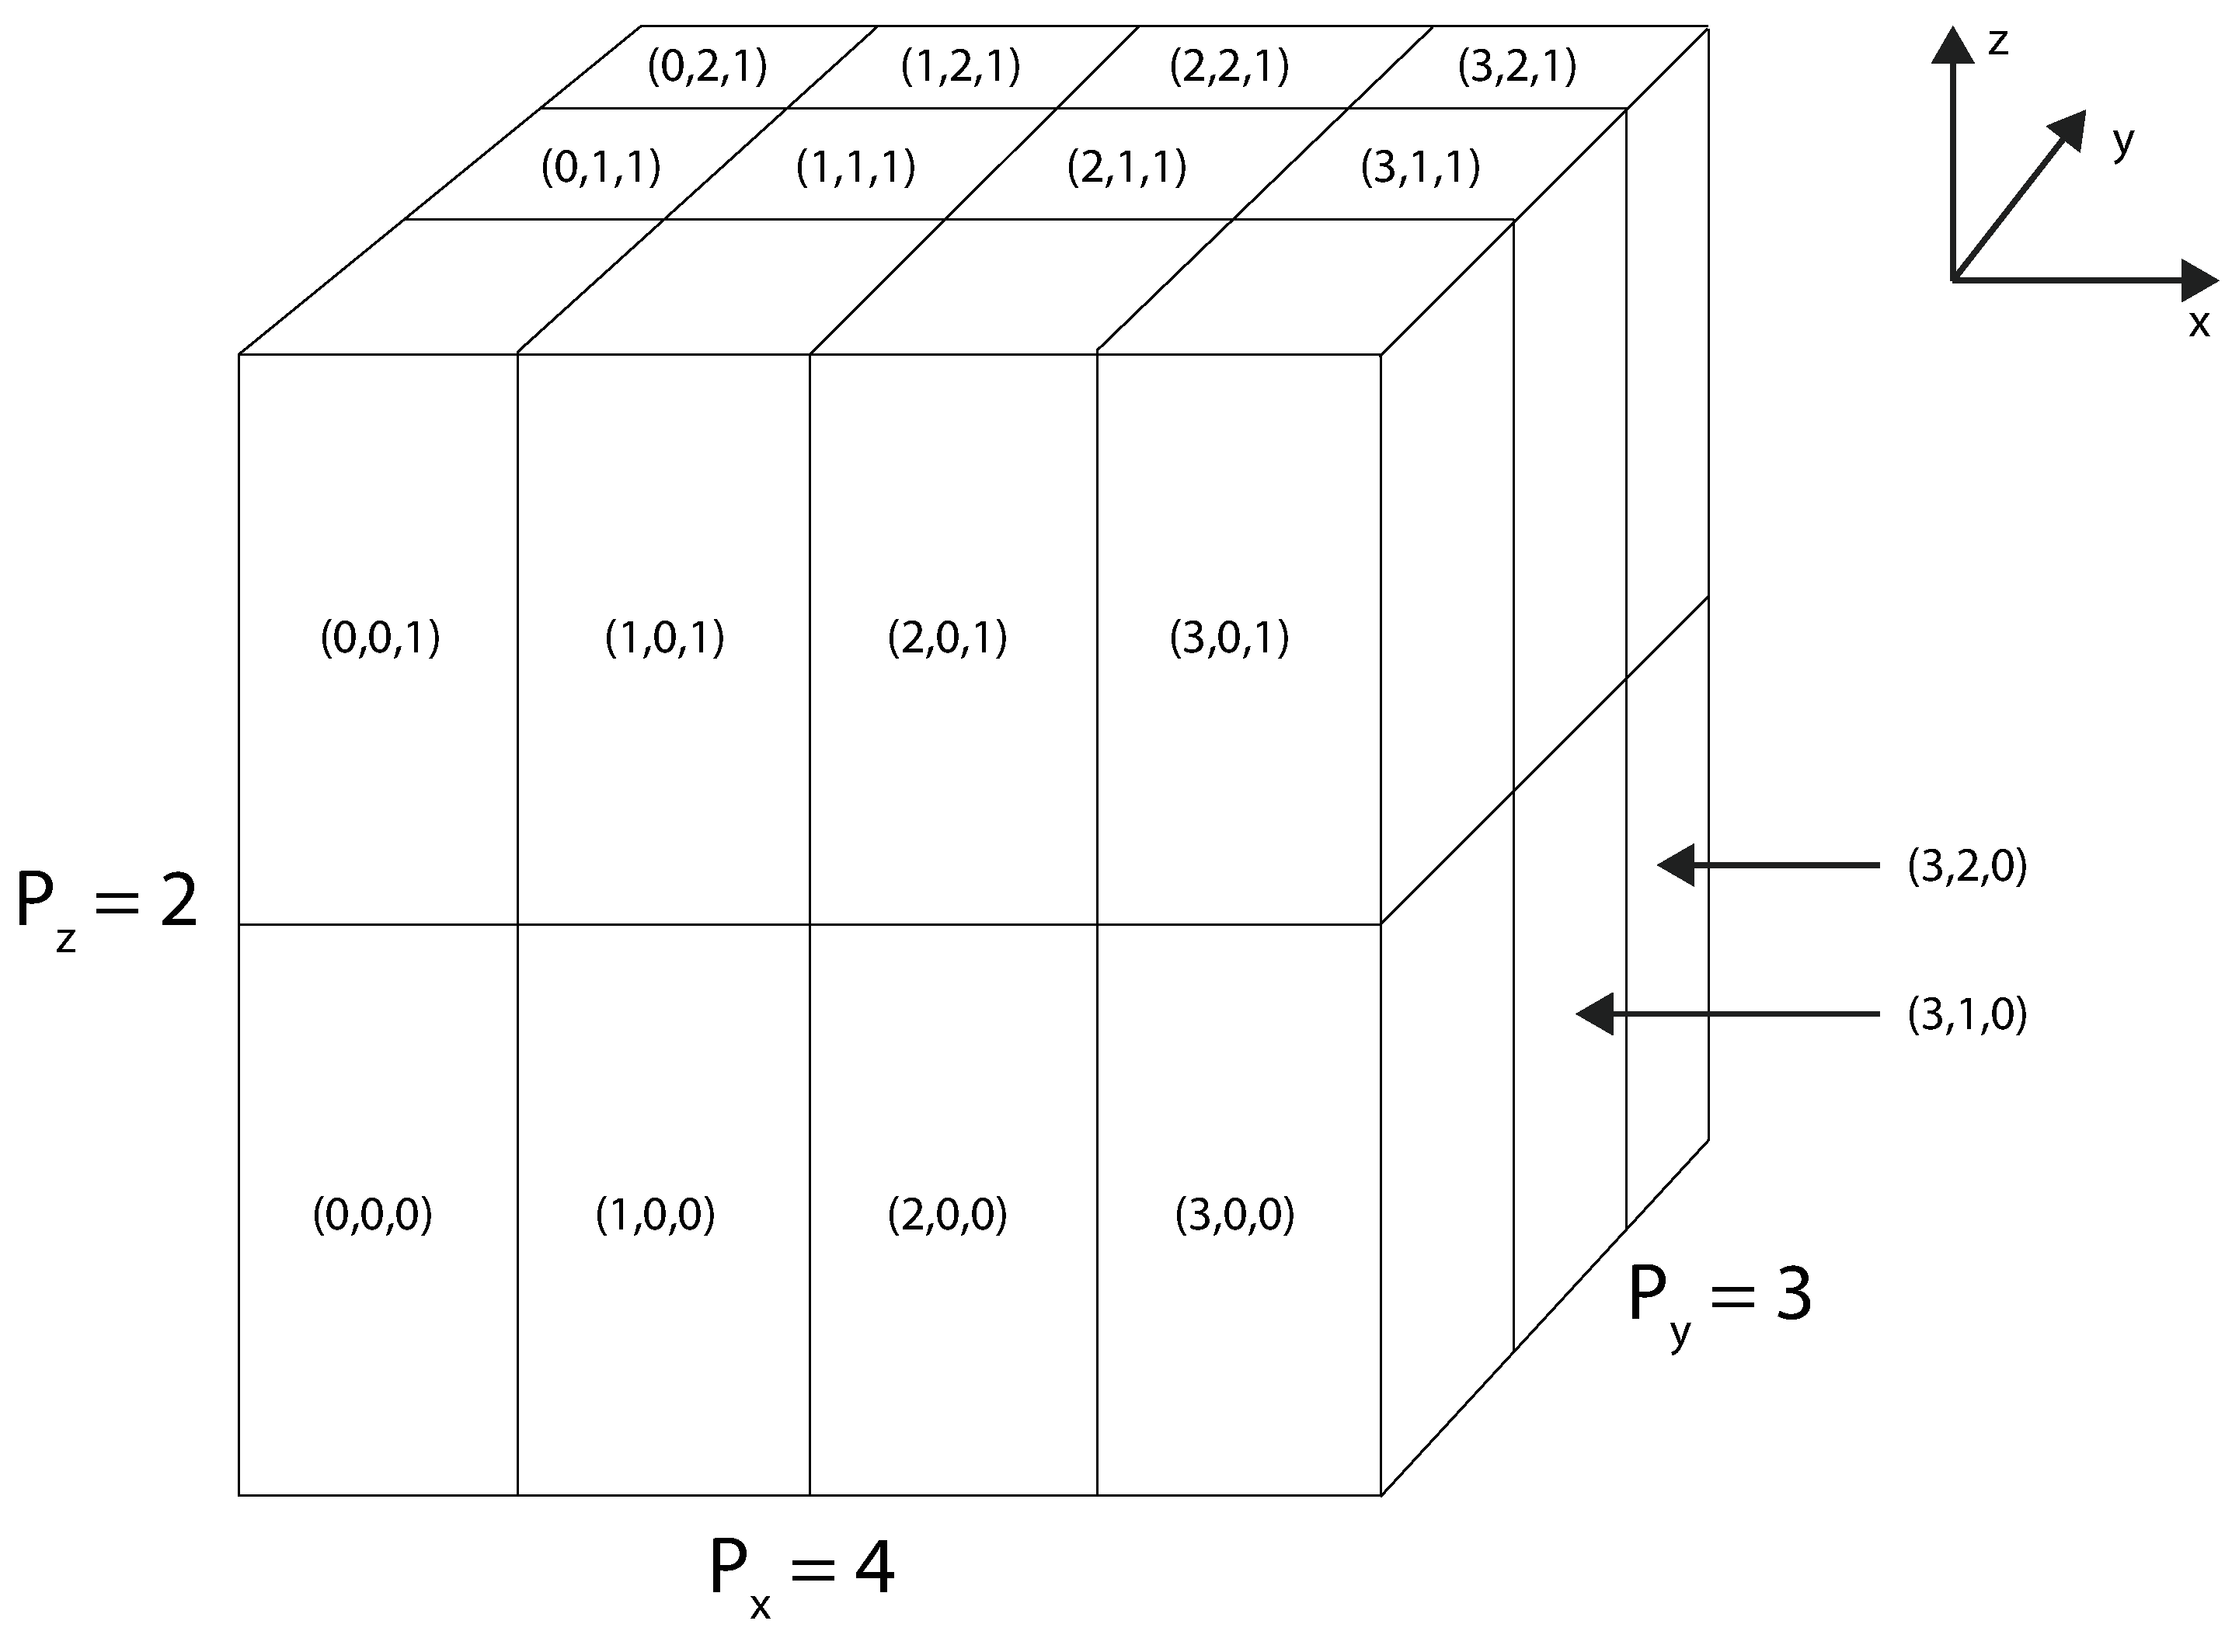
\includegraphics[width=0.7\textwidth, trim=0cm 0cm 0cm 0cm, clip]{DSMC/figures/parallelization_node_configuration.eps}
\end{center}
\caption{Processor labelin up in a 3-dimensionizzle grid. Y'all KNOW dat shit, muthafucka! Each processor is uniquely identified all up in its coordinizzle $(p_x, p_y, p_z)$.}
\label{fig:md_parallelization_2}
\end{figure}
We represent tha coordinatez of a atom on processor $(p_x, p_y, p_z)$ up in tha local coordinizzle system where tha CPUz origin $\vec p_\text{origin}$ defines tha coordinizzle system fo' realz. An atom wit global coordinates $\vec r$ will then have local coordinates $\vec r'$
\begin{align}
	\vec r' = \vec r - \vec p_\text{origin}.
\end{align}
We can then easily detect if a atom has moved outside its processorz domain by checkin if any of tha local coordinizzle components is outside tha range $[0, l_i)$ fo' dimension $i$. If a atom has moved ta another processor, it has moved ta one of tha 26 neighborin processors. Us thugs will use tha same 3-step process as busted lyrics bout up in subsection \ref{sec:dsmc_parallelization_exchange_particles} which is dopest illustrated wit tha 2-dimensionizzle example up in figure \ref{fig:md_parallelization_facet_technique}.
\begin{figure}[h!]
\begin{center}
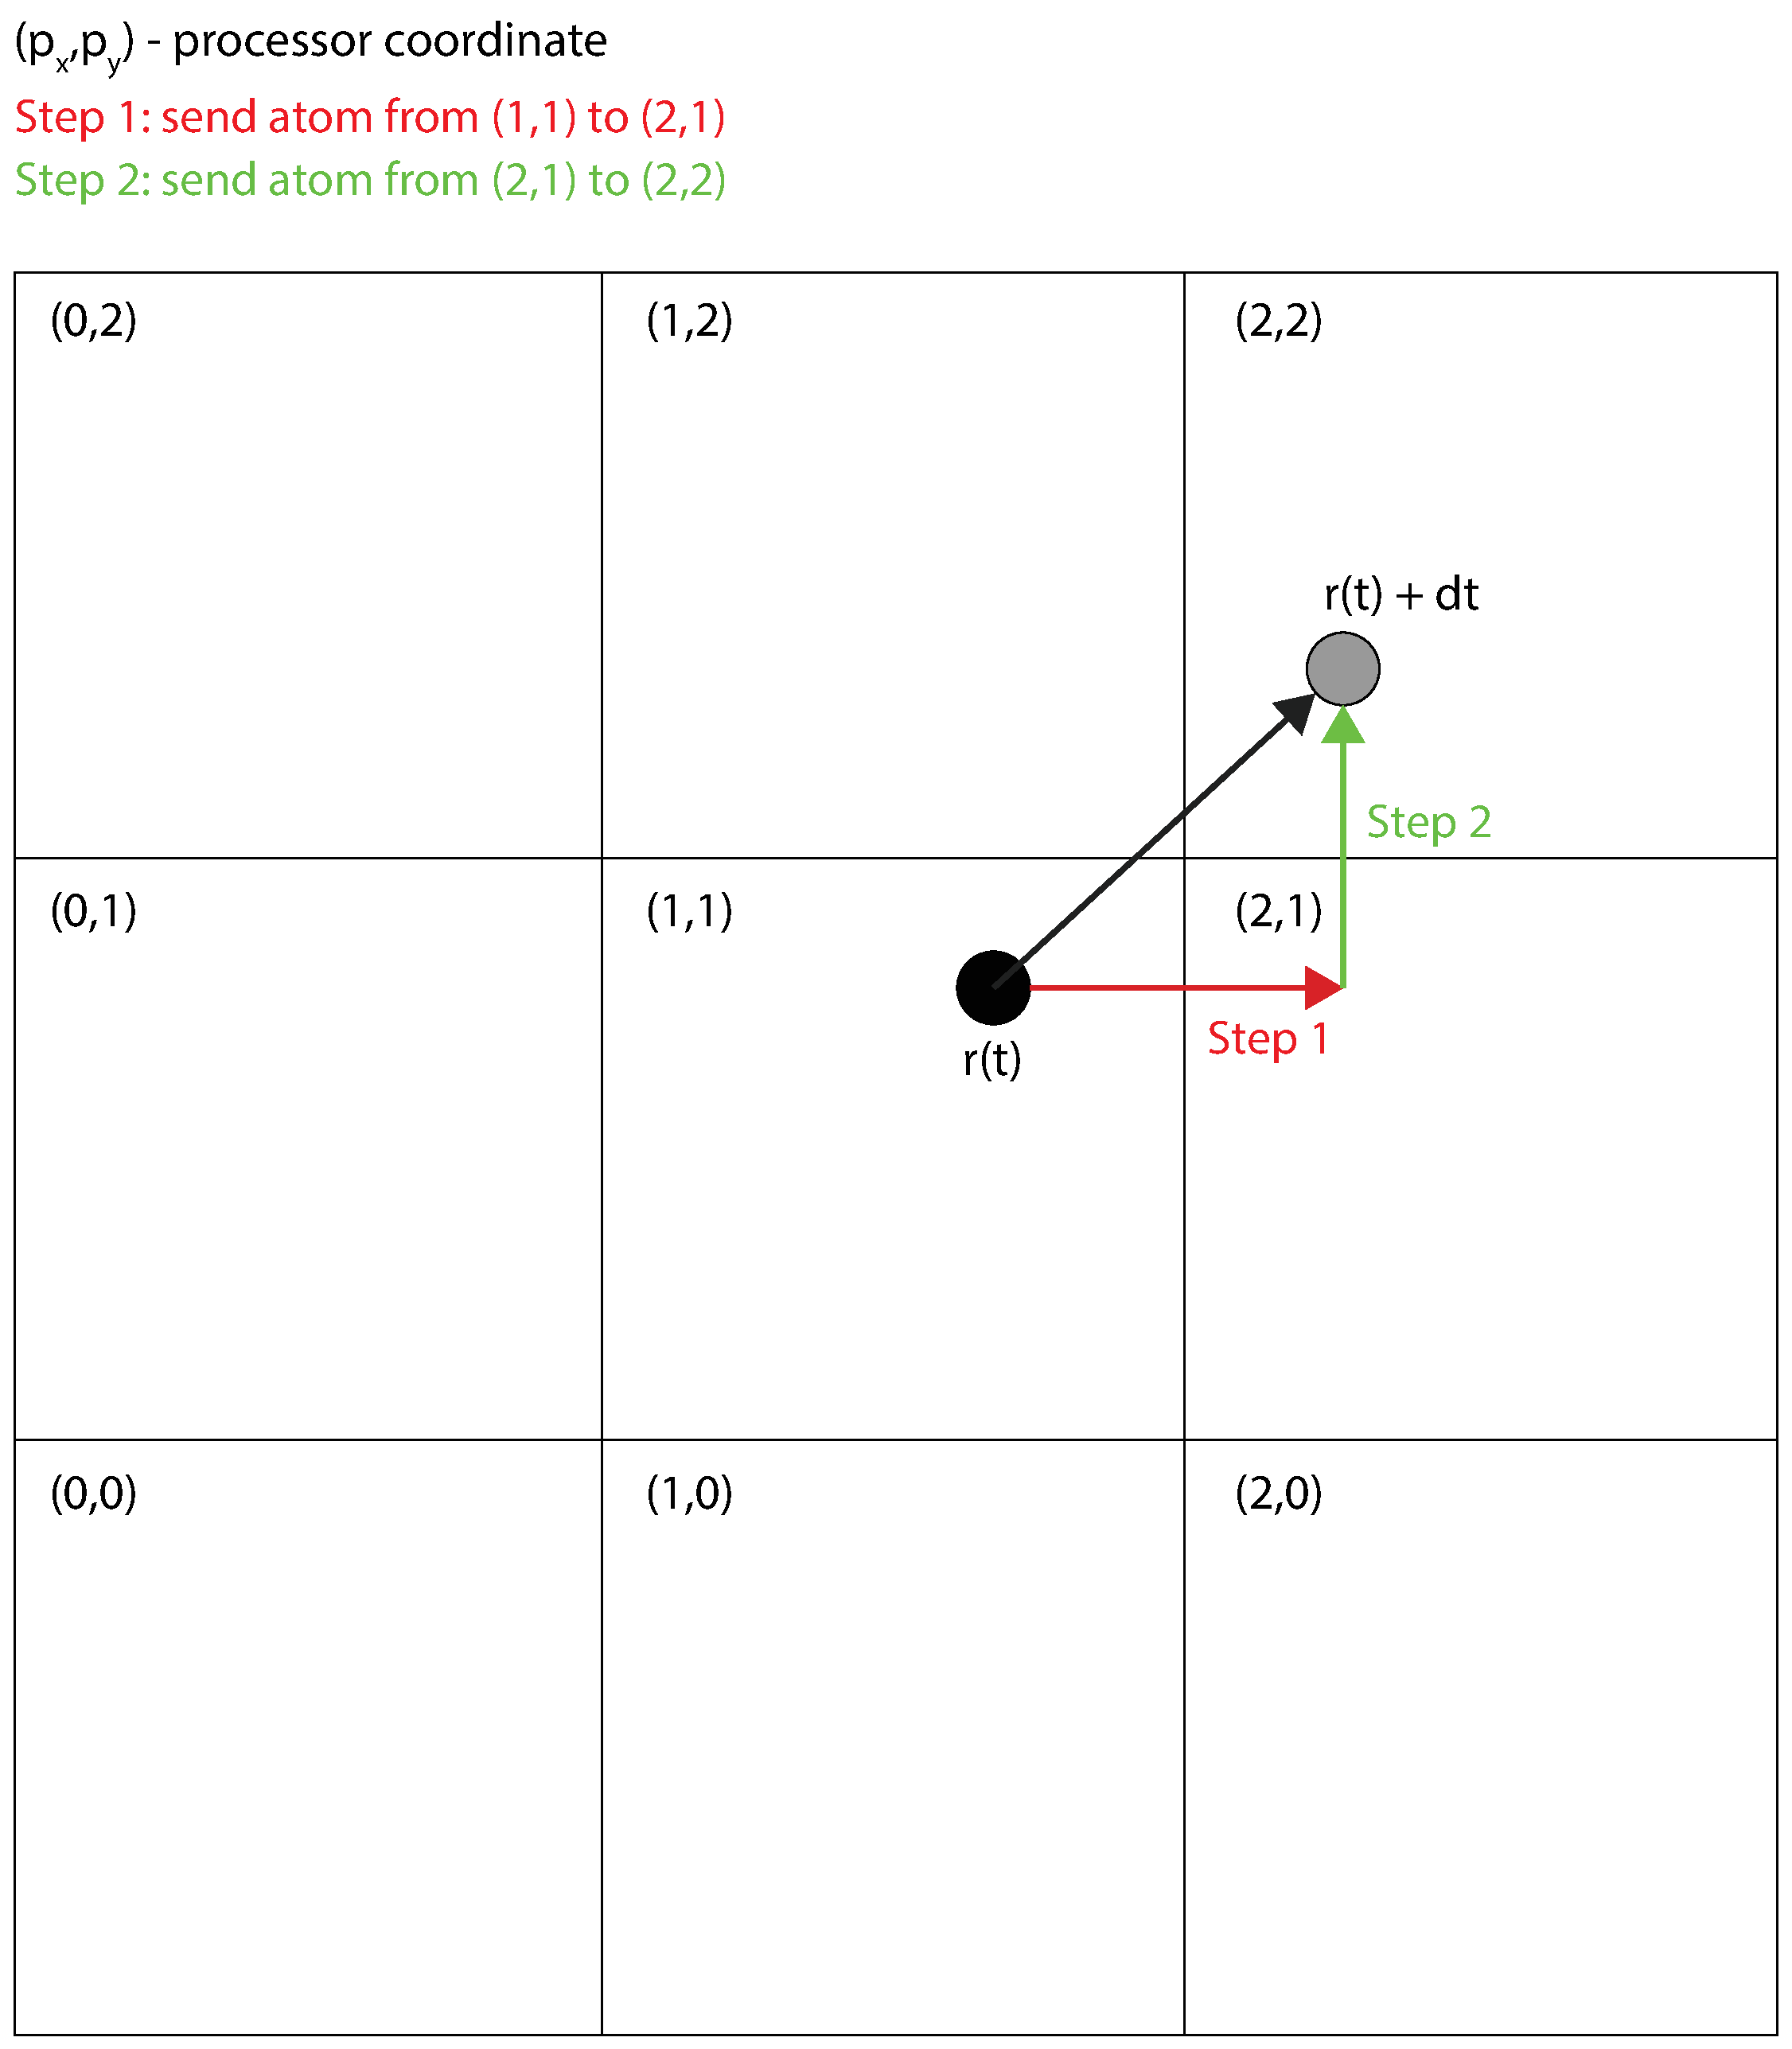
\includegraphics[width=0.7\textwidth, trim=0cm 0cm 0cm 0cm, clip]{MD/figures/parallelization_facet_technique.eps}
\end{center}
\caption{Da middle node (1,1) has 8 neighbors it need ta rap with. Each node only need ta rap wit its nearest neighbors (4 up in two dimensions, 6 up in three dimensions), cuz tha nearest neighbors can work as intermediate shiznit carriers fo' realz. An atom movin from processor (1,1) ta (2,2) will up in step 1 be busted ta (2,1), then up in step 2 be busted ta (2,2).}
\label{fig:md_parallelization_facet_technique}
\end{figure}
We only need ta know bout tha 6 nearest neighbors on each processor. Shiiit, dis aint no joke. We notice a neat detail here, periodic boundary conditions is automatically taken care of. If we again n' again n' again peep figure \ref{fig:md_parallelization_2}, our crazy asses have 4 processors up in tha $x$-direction. I aint talkin' bout chicken n' gravy biatch. Da processor ta tha \textit{right} of $(3,0,1)$ is $(0,0,1)$ if we use periodic boundary conditions. But since we use tha local coordinates on each processor, when a atom moves ta another processor, its coordinates must be \textit{shifted} so its has erect local coordinates on tha freshly smoked up processor. Shiiit, dis aint no joke. Each processor has one \textit{shift vector} per neighbor, containin tha transformation it need ta apply on tha atomz coordinates before it moved. Y'all KNOW dat shit, muthafucka! If tha atom moved all up in tha system boundary (periodic boundary conditions), tha shift vector must of course reflect all dis bullshit. 
    \section{Pressure driven flows}
We will induce flow in the same way we did in section \ref{sec:dsmc_pressure_driven_flows}. We apply a 
    \section{Complex geometries}
As we did with DSMC, we want to study flow in arbitrary geometries.  To be able to do this, we need to create a model that satisfies some properties we already have in DSMC. The flowing fluid needs to
\begin{itemize}
	\item be confined in a subset of the total volume
	\item have realistic interactions with the solid wall
	\item have energy drained by the solid.
\end{itemize}
The first requirement is not completely strict, but most of the flowing fluid should be in the free volume. The reason why we need to drain the energy is that in order to induce fluid flow, we will apply a constant force that increases the total energy of the system. We want to reach an equilibrium where the average rate of drained energy exactly matches the energy from the applied force. We assume that the geometry is described as a boolean function $G : \mathcal(R)^3\rightarrow \{1,0\}$ that fully determines whether a point in space is part of the solid or the free volume. A convinient representation is the voxelization described in section \ref{sec:dsmc_binary_representation}. 
\subsection{A naive approach}
To illustrate the basic idea, we will discuss the simplest model satisfying only the first two requirements. Given a molecular dynamics state, we can loop through the positions $\vec r_i$ of each atom $i$, and mark the atoms as \textit{frozen} if $G(\vec r_i) = 1$ (which means that this point is part of the solid). Atoms marked as frozen will not move at all, but all forces are calculated normally. One way of interpreting the non-moving frozen atoms is that they have infinite mass. The total energy is still conserved in the system. An implementation is illustrated in listing \ref{lst:md_simple_solid}.

\begin{lstlisting}[caption=Example code showing how to mark atoms within a solid., label=lst:md_simple_solid]
bool point_is_a_solid(double *position) {
	int voxel_index_i = position[0] / system_length[0] * num_voxels[0];
	int voxel_index_j = position[1] / system_length[1] * num_voxels[1];
	int voxel_index_k = position[2] / system_length[2] * num_voxels[2];

	// The world matrix is a binary matrix
	return world_matrix[voxel_index_i, voxel_index_j, voxel_index_k];
}

void mark_frozen_atoms() {
	for(int i=0; i<num_atoms; i++) {
		double *position = positions[i];
		if(point_is_a_solid(position)) {
			atom_types[i] = FROZEN;
		}
	}
}

void move() {
	for(int i=0; i<num_atoms; i++) {
		if(atom_types[i] != FROZEN) {
			positions[i][0] += velocities[i][0];
			positions[i][1] += velocities[i][1];
			positions[i][2] += velocities[i][2];
		}
	}
}
\end{lstlisting}
If the atoms forming the solid are dense enough, very few atoms will be inside the wall, so the first requirement is satisfied. The interaction between the solid and the flowing fluid is as realistic as the potential is, so the only requirement not satisfied is the drainage of the energy. In figure \ref{fig:md_simplesolid}, we see how the red flowing atoms are confined within a cylinder with radius $R$. 

\begin{figure}[h]
\begin{center}
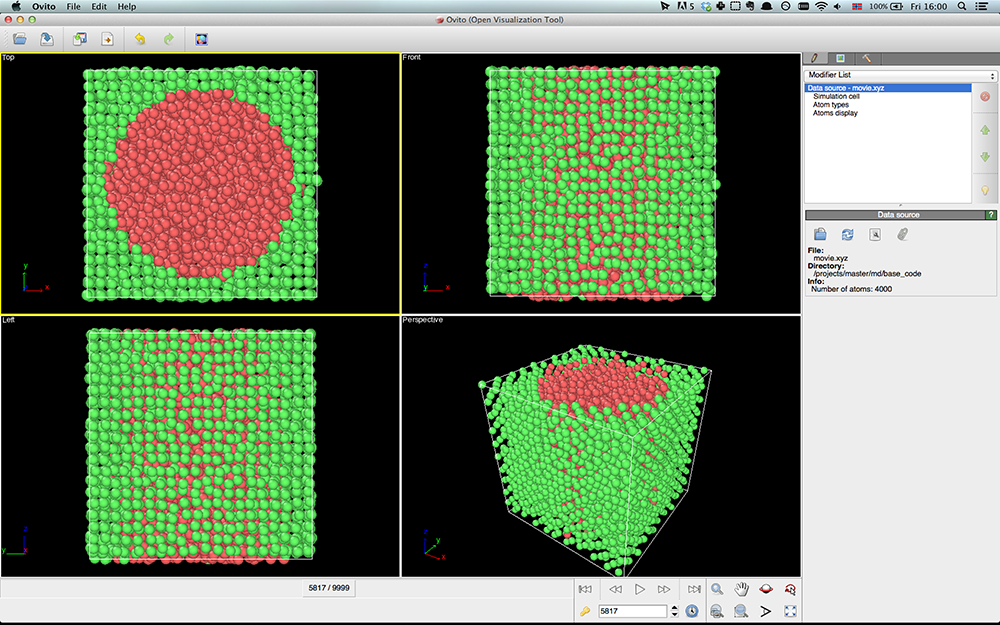
\includegraphics[width=1.0\textwidth, trim=0cm 0cm 0cm 0cm, clip]{MD/figures/solid_model.png}
\label{fig:md_simple_solid}
\end{center}
\caption{A simple model of a solid where the green atoms are frozen confining the red flowing atoms within a cylinder of radius $R$. The visualization is done in Ovito.}
\end{figure}

\subsection{A simple model of a solid}
We can improve the solid model by adding a harmonic oscillator potential to all the frozen atoms. Instead of freezing them completely, we allow them to vibrate around their equilibrium position $\vec q$ which is the initial position of the simulation. The force on atom $i$ in the solid is then
\begin{align}
	F^{(s)}(\vec r_i) = -k(\vec r_i - \vec q_i) 
	- \sum_{j\neq i} 24\epsilon\left[2\left(\frac{\sigma^{12}}{r_{ij}^{13}}\right) - \left(\frac{\sigma^6}{r_{ij}^7}\right)\right]\vec u_{ij},
\end{align}
where $k$ is the strength of the oscillator, $\vec q_i$ is the equilibrium position for atom $i$ and the last part is the Lennard-Jones potential described in section \ref{sec:md_lj_potential}.\\
\subsubsection{Energy drainage}
The energy is of course still conserved with this model, but we can now apply a thermostat on the atoms in the solid making them act as a large reservoir trying to keep the temperature at some wall temperature $T_w$. With this model, we can study flow in any geometry with a behaviour near that of the DSMC model. An implementation is shown in listing \ref{lst:md_ho_solid}.

\begin{lstlisting}[caption=Implementation of the harmonic oscillator model of a solid., label=lst:md_ho_solid]

void apply_gravity() {
    for(n=0;n<num_atoms;n++) {
        if(atom_type[n] != FROZEN) velocities[n][gravity_direction] += gravity_acceleration*dt;
    }
}

void apply_harmonic_oscillator() {
    double spring_constant = 1000.0;
    for(n=0; n<num_atoms; n++) {
        if(atom_type[n] == FROZEN) {
            double dx = positions[n][0] - initial_positions[n][0];
            double dy = positions[n][1] - initial_positions[n][1];
            double dz = positions[n][2] - initial_positions[n][2];
            accelerations[n][0] += -spring_constant*dx / mass;
            accelerations[n][1] += -spring_constant*dy / mass;
            accelerations[n][2] += -spring_constant*dz / mass;
        }
    }
}

void step() {
    move();
    apply_gravity();
    apply_lennard_jones();
    apply_harmonic_oscillator();
    update_velocities();
}
\end{lstlisting}
  \end{chapter}

  \begin{chapter}{Validation and results}
    \section{Validation}
    In this chapter we discuss the results of our MD simulations. Here we start by a scaling performance benchmark in section \ref{sec:md_benchmark} before we in section \ref{sec:md_cylinder_result} move on to a validation of the Knudsen correction we confirmed with the DSMC model. Most of the concepts are equivalent as in DSMC in section \ref{sec:dsmc_parallelization_performance}, so the reader is is assumed to have read that section.

\section{Parallelization performance}
\label{sec:md_benchmark}
The parallelization scheme we have used in MD is very similar to the one we used in DSMC. In section \ref{sec:dsmc_parallelization_performance}, we measured both the strong and the weak scaling efficiency ($\eta_s$ and $\eta_w$) which measure two different ways of scaling the program. We will not repeat the discussion about these except present the result for both scaling for the MD program. 

\subsection{Strong scaling}
The strong scaling efficiency $\eta_s$ tells us how well the program scales if we keep the system size constant while increasing the number of processors. The strong scaling efficiency was defined as
\begin{align}
	\eta_s = \frac{t_1}{Nt_N},
\end{align}
where $t_1$ is the total run time using one processor and $t_N$ is the total run time using $N$ processors. In this benchmark, we chose a system consisting of $48\times48\times48=110592$ unit cells which gives a total of 442368 atoms. When we increase the number of processors, these 48 unit cells per dimension are distributed on the processors. The timestep was $\Delta t = 0.02$ and the initial temperature was approximately $T_0=$\unit{100}{\kelvin} so that the final gas temperature was around $T=$\unit{60}{\kelvin}. This fall in temperature is explained by the fact that the FCC lattice is the potential minimum, so with a non-zero temperature, some of the initial kinetic energy will be converted to potential energy. We run the program with the number of processors in the range 1 to 512. In table \ref{tab:md_strong_scaling} we have presented the results for this benchmark which is summarized in figure \ref{fig:md_strong_scaling}. We see that when going from one to two processors, we get a more than ideal speedup with $\eta_s(N_\text{CPU}=2)=1.17$ which can be explained by the CPU cache. When a processor compute with a value stored at some memory address, it will first look in the three levels of cache to see if the value of the memory address is cached there. Cached values are much faster available for computation than those only in the memory. When going from one processor to two, a larger part of the positions array (which is used in the force calculation) can be cached, hence a more than double speedup is obtainable. When using a larger number of processors, the MPI communication time starts increasing so that the total time increases per cpu. 

\begin{table}[h]
\begin{center}
    \begin{tabular}{|l|l|l|l|l|}
    \hline
    $N_\text{CPU}$ & $N_\text{atoms}/N_\text{CPU}$ & $t_N$ & $\eta_s$ \\ \hline
    1 & 442368 & \unit{29196}{\second} & 1.00\\
    \hline
    2 & 221184 & \unit{12471}{\second} & 1.17\\
    \hline
    4 & 110592 & \unit{6435}{\second} & 1.13\\
    \hline
    8 & 55296 & \unit{3469}{\second} & 1.05\\
    \hline
    16 & 27648 & \unit{1926}{\second} & 0.95\\
    \hline
    32 & 13824 & \unit{1021}{\second} & 0.89\\
    \hline
    64 & 6912 & \unit{715}{\second} & 0.64\\
    \hline
    128 & 3456 & \unit{375}{\second} & 0.61\\
    \hline
    256 & 1728 & \unit{220}{\second} & 0.52\\
    \hline
    512 & 864 & \unit{150}{\second} & 0.38\\
    \hline
    \end{tabular}
    \caption{Benchmark results showing the strong scaling efficiency $\eta_s$ for the MD program. We see that when going from one to two processors, we get a more than ideal speedup with $\eta_s(N_\text{CPU}=2)=1.17$ which can be explained by the CPU cache. When a processor compute with a value stored at some memory address, it will first look in the three levels of cache to see if the value of the memory address is cached there. Cached values are much faster available for computation than those only in the memory. When going from one processor to two, a larger part of the positions array (which is used in the force calculation) can be cached, hence a more than double speedup is obtainable. When using a larger number of processors, the MPI communication time starts increasing so that the total time increases per cpu.}
    \label{tab:md_strong_scaling}
    \end{center}
\end{table}

\begin{figure}[h!]
\begin{center}
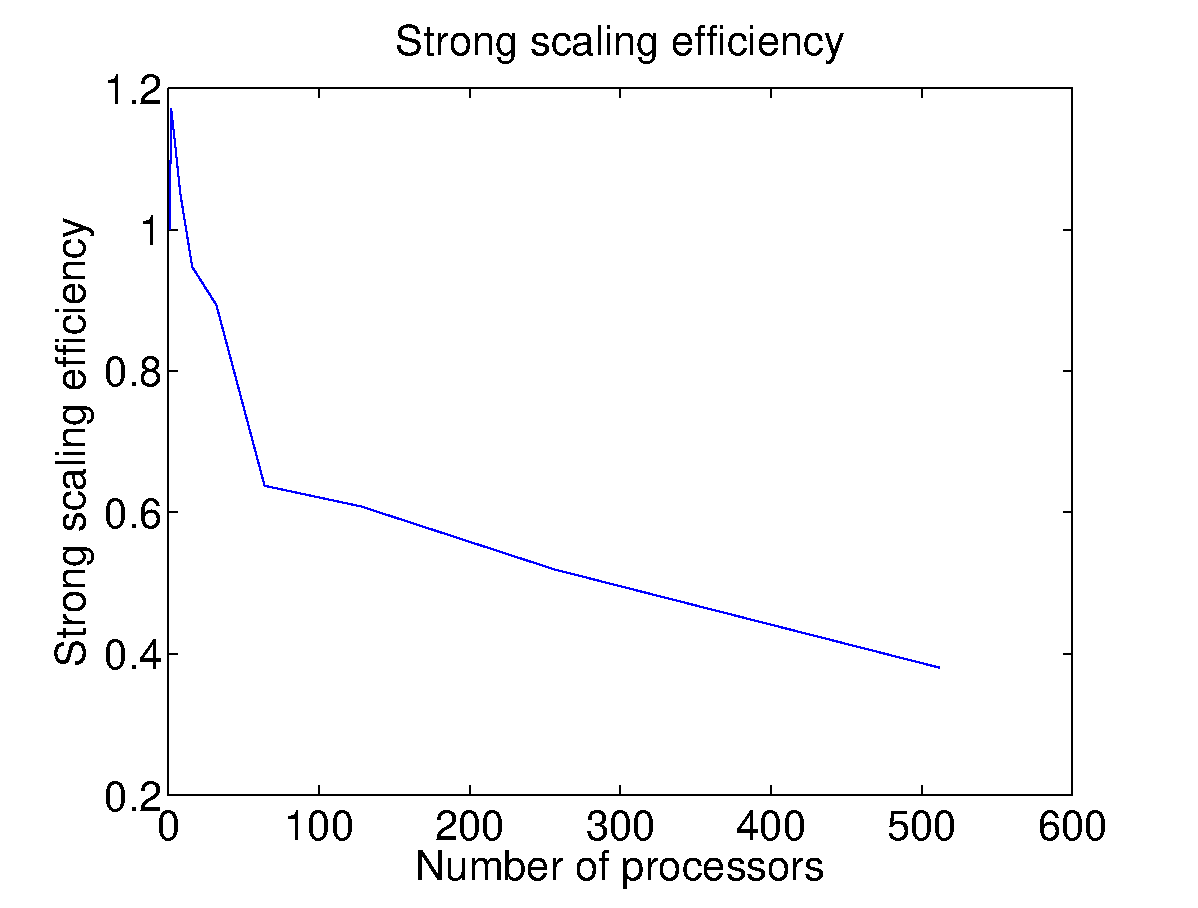
\includegraphics[width=0.7\textwidth, trim=0cm 0cm 0cm 0cm, clip]{MD/figures/strong_scaling.eps}
\end{center}
\caption{Benchmark results showing the strong scaling efficiency $\eta_s$ for the MD program. We see that when going from one to two processors, we get a more than ideal speedup with $\eta_s(N_\text{CPU}=2)=1.17$ which can be explained by the CPU cache. When a processor compute with a value stored at some memory address, it will first look in the three levels of cache to see if the value of the memory address is cached there. Cached values are much faster available for computation than those only in the memory. When going from one processor to two, a larger part of the positions array (which is used in the force calculation) can be cached, hence a more than double speedup is obtainable. When using a larger number of processors, the MPI communication time starts increasing so that the total time increases per cpu.}
\label{fig:md_strong_scaling}
\end{figure}

\subsection{Weak scaling}
If we increase the number of processors, but keep the nubmer of atoms per processor constant, we can use the weak scaling efficiency $\eta_w$ to see how the program scales in this case. The weak scaling efficiency is defined as
\begin{align}
	\eta_w = \frac{t_1}{t_N},
\end{align}
where again $t_1$ is the total run time using one processor and $t_N$ is the run time using $N$ processors. In this benchmark, we chose $10\times10\times10=1000$ unit cells per processor yielding a total of 4000 atoms per cpu. The timestep here as well is $\Delta t = 0.02$ with the same initial temperature as in the strong scaling so that the final temperature is approximately $T=$\unit{60}{\kelvin}. In table \ref{tab:md_weak_scaling} and figure \ref{fig:md_weak_scaling}, we have presented the results for the weak scaling. 

\begin{table}[h]
\begin{center}
    \begin{tabular}{|l|l|l|l|l|}
    \hline
    $N_\text{CPU}$ & $N_\text{atoms}$ & $t_N$ & $\eta_w$ \\ \hline
    1 & 4000 & \unit{1246}{\second} & 1.00\\
    \hline
    2 & 8000 & \unit{1278}{\second} & 0.97\\
    \hline
    4 & 16000 & \unit{1398}{\second} & 0.89\\
    \hline
    8 & 32000 & \unit{1441}{\second} & 0.86\\
    \hline
    16 & 64000 & \unit{1521}{\second} & 0.82\\
    \hline
    32 & 128000 & \unit{1620}{\second} & 0.77\\
    \hline
    64 & 256000 & \unit{1639}{\second} & 0.76\\
    \hline
    128 & 512000 & \unit{1735}{\second} & 0.72\\
    \hline
    256 & 1024000 & \unit{2027}{\second} & 0.61\\
    \hline
    512 & 2048000 & \unit{3379}{\second} & 0.37\\
    \hline
    \end{tabular}
    \caption{Benchmark results showing the weak scaling efficiency $\eta_w$ for the MD program. }
    \label{tab:md_weak_scaling}
    \end{center}
\end{table}

\begin{figure}[h!]
\begin{center}
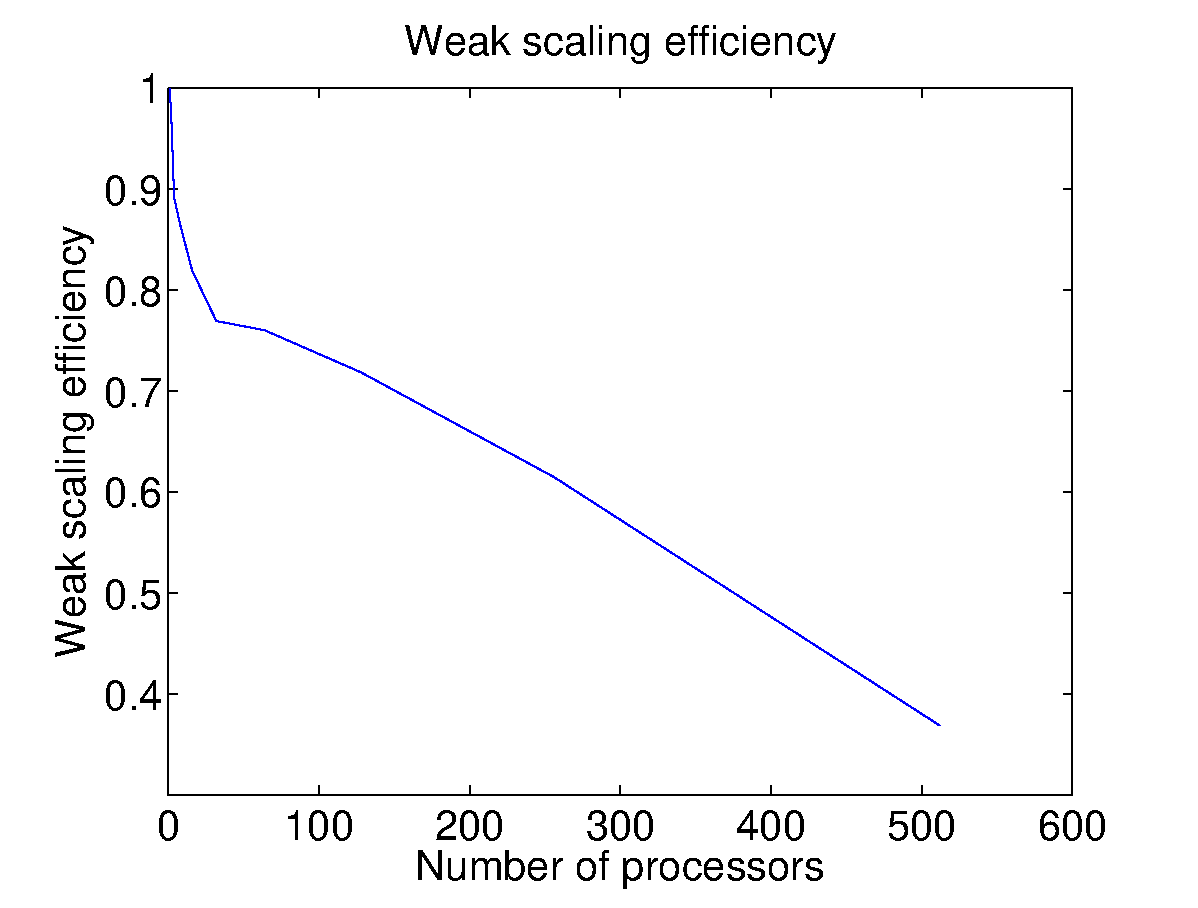
\includegraphics[width=0.7\textwidth, trim=0cm 0cm 0cm 0cm, clip]{MD/figures/weak_scaling.eps}
\end{center}
\caption{Benchmark results showing the weak scaling efficiency $\eta_w$ for the MD program.}
\label{fig:md_weak_scaling}
\end{figure}

\section{Flow in a cylinder, varying Knudsen number}
\label{sec:md_cylinder_result}
We have used the MD program to simulate flow in a cylinder with a fixed radius $R$, just like we did in section \ref{sec:results_for_simple_geometries} with DSMC. We will measure the permeability to see how well the Knudsen correction factor (see section \ref{sec:knudsen_correction}) predicts the permeability for very small pores (here a cylinder) with an atomic model. The cylinder was created with the solid model we described in section \ref{sec:md_simple_model_of_a_solid}. Since the solid now consists of atoms (in DSMC it was just a scalar field defining the surface), we should create the cylinder carefully. We have prepared the system with the following steps
\begin{itemize}
	\item Heat the system 2000 timesteps, $T=$\unit{300}{\kelvin}
	\item Thermalize the system 2000 timesteps
	\item Heat the system 2000 timesteps, $T=$\unit{300}{\kelvin}
	\item Thermalize the system 2000 timesteps
	\item Create cylinder (explained below)
	\item Reduce density (explained below).
\end{itemize}
By first heating the system, we let the system melt from a solid state to a liquid state. This allows the system to become more random than in the initial lattice. Once we create the cylinder, we apply a harmonic oscillator potential on the atoms in the cylinder so they more or less stay in their initial position. We have here chosen a system consisting of $64\times64\times64=262144$ unit cells which gives a total of 1048576 atoms to begin with. This in turn yields a system with size $L_i=336.64Å$ in the $i$th dimension. By choosing the cylinder radius to be $r=0.45L_i$ and the flow in the $z$-direction, we mark all atoms within a distance $r$ from the center (in the $xy$-plane) as gas atoms, and atoms outside $r$ as solid atoms. But the cut-off radius was chosen to be $r_\text{cut}=2.5\sigma$ (see section \ref{sec:md_implementation_two_body_forces}), so the gas atoms inside the cylinder will not feel the precense of the atoms outside $r+2.5\sigma$ directly. To save computation time, we have removed all atoms outside this radius. Such a cylinder is shown in figure \ref{fig:md_cylinder} where the yellow atoms are the solid wall wheras the green atoms are the gas.
\begin{figure}[h!]
\begin{center}
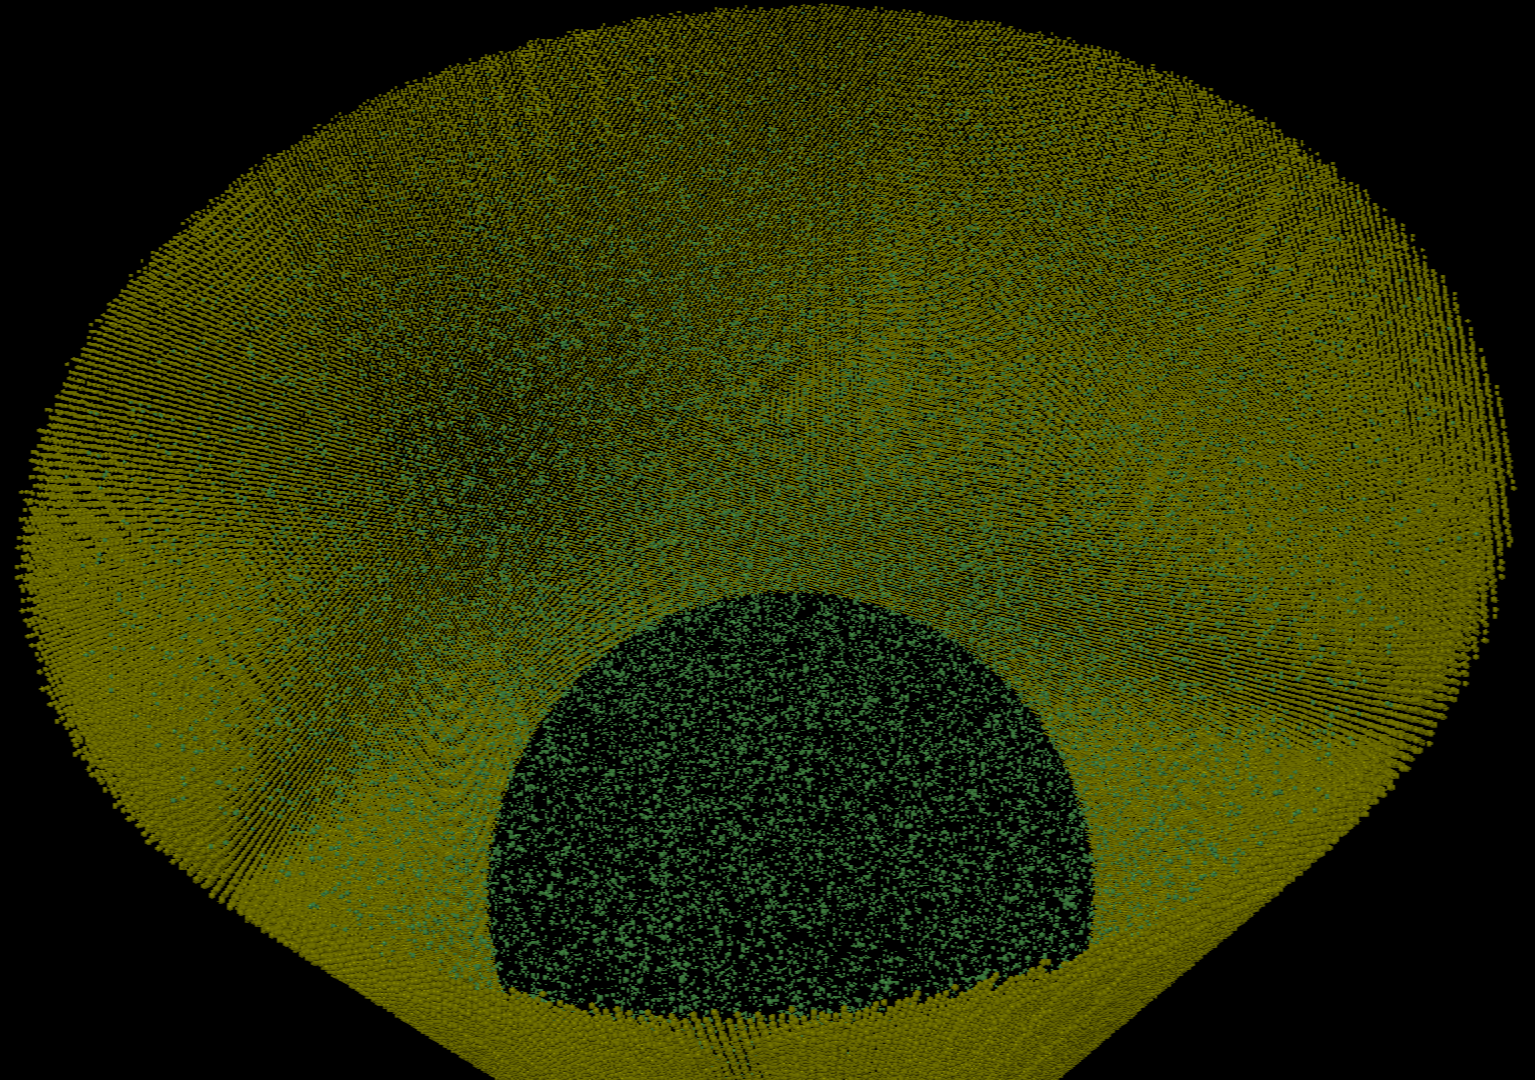
\includegraphics[width=0.8\textwidth, trim=0cm 0cm 0cm 0cm, clip]{MD/figures/md_cylinder.png}
\end{center}
\caption{The final cylinder we used to simulate gas to validate the Knudsen correction factor for the permeability (see section \ref{sec:knudsen_correction}). Here the yellow atoms are the solid wall (with a harmonic oscillator potential on each atom, keeping the atoms in place), and the green atoms are the gas. Since we have used a cut-off radius $r_\text{cut}=2.5\sigma$, we have removed the solid atoms outside the radius $r+2.5\sigma$. This visualization is done with the tool discussed and developed in chapter \ref{chap:particle_visualizer}.}
\label{fig:md_cylinder}
\end{figure}
Once we have the cylinder, we can choose the density yielding a desired Knudsen number
\begin{align}
	\rho_n(\text{Kn}) = \frac{1}{\sqrt 2 \pi d^2 \text{Kn}L},
\end{align}
where we have used $d=$\unit{3.62}{\angstrom} as we did in DSMC. The flow is induced in the same way as we did in DSMC (explained in section \ref{sec:dsmc_pressure}), where we can, given a pressure difference $\Delta P$, accelerate the atoms inside the cylinder according to equation \eqref{eq:acceleration_to_pressure_difference}
\begin{align*}
	g = \frac{\Delta P}{\rho_m\Delta x}.
\end{align*}
Here, $\Delta x$ is the system length in the flow direction, $L_z$. We have chosen a pressure difference equal to $0.2P_0$, where $P_0=\rho_nk_BT$ being the ideal gas pressure. We can then for each Knudsen number induce flow and measure the permeability. The system reached an equilibrium state before we sampled for $500000$ timesteps. In figure \ref{fig:md_permeability}, we have plotted the measured permeabilities for different Knudsen numbers with the Knudsen corrected analytical solution
\begin{align}
	\label{eq:cylinder_knudsen_corrected}
	k_a = [1 + \alpha(\text{Kn})\text{Kn}]\left[1 + {4\text{Kn}\over 1 + \text{Kn}}\right] {r^2\over 8}.
\end{align}
The left figure, using a logarithmic $x$-axis shows that the permeabilities in the lower range of the Knudsen numbers are predicted very by the theory. The right figure shows that the permeabilities in the whole range, two orders of magnitues, follows the expression in equation \eqref{eq:cylinder_knudsen_corrected}. For the high Knudsen numbers, we see an increase in the statistical noise which is explained by the fact that a high Knudsen number is obtained by a low density which gives a low number of atoms. In order to get better statistics, we would need to run the simulation for a longer time.
\begin{figure}[h]
\begin{center}
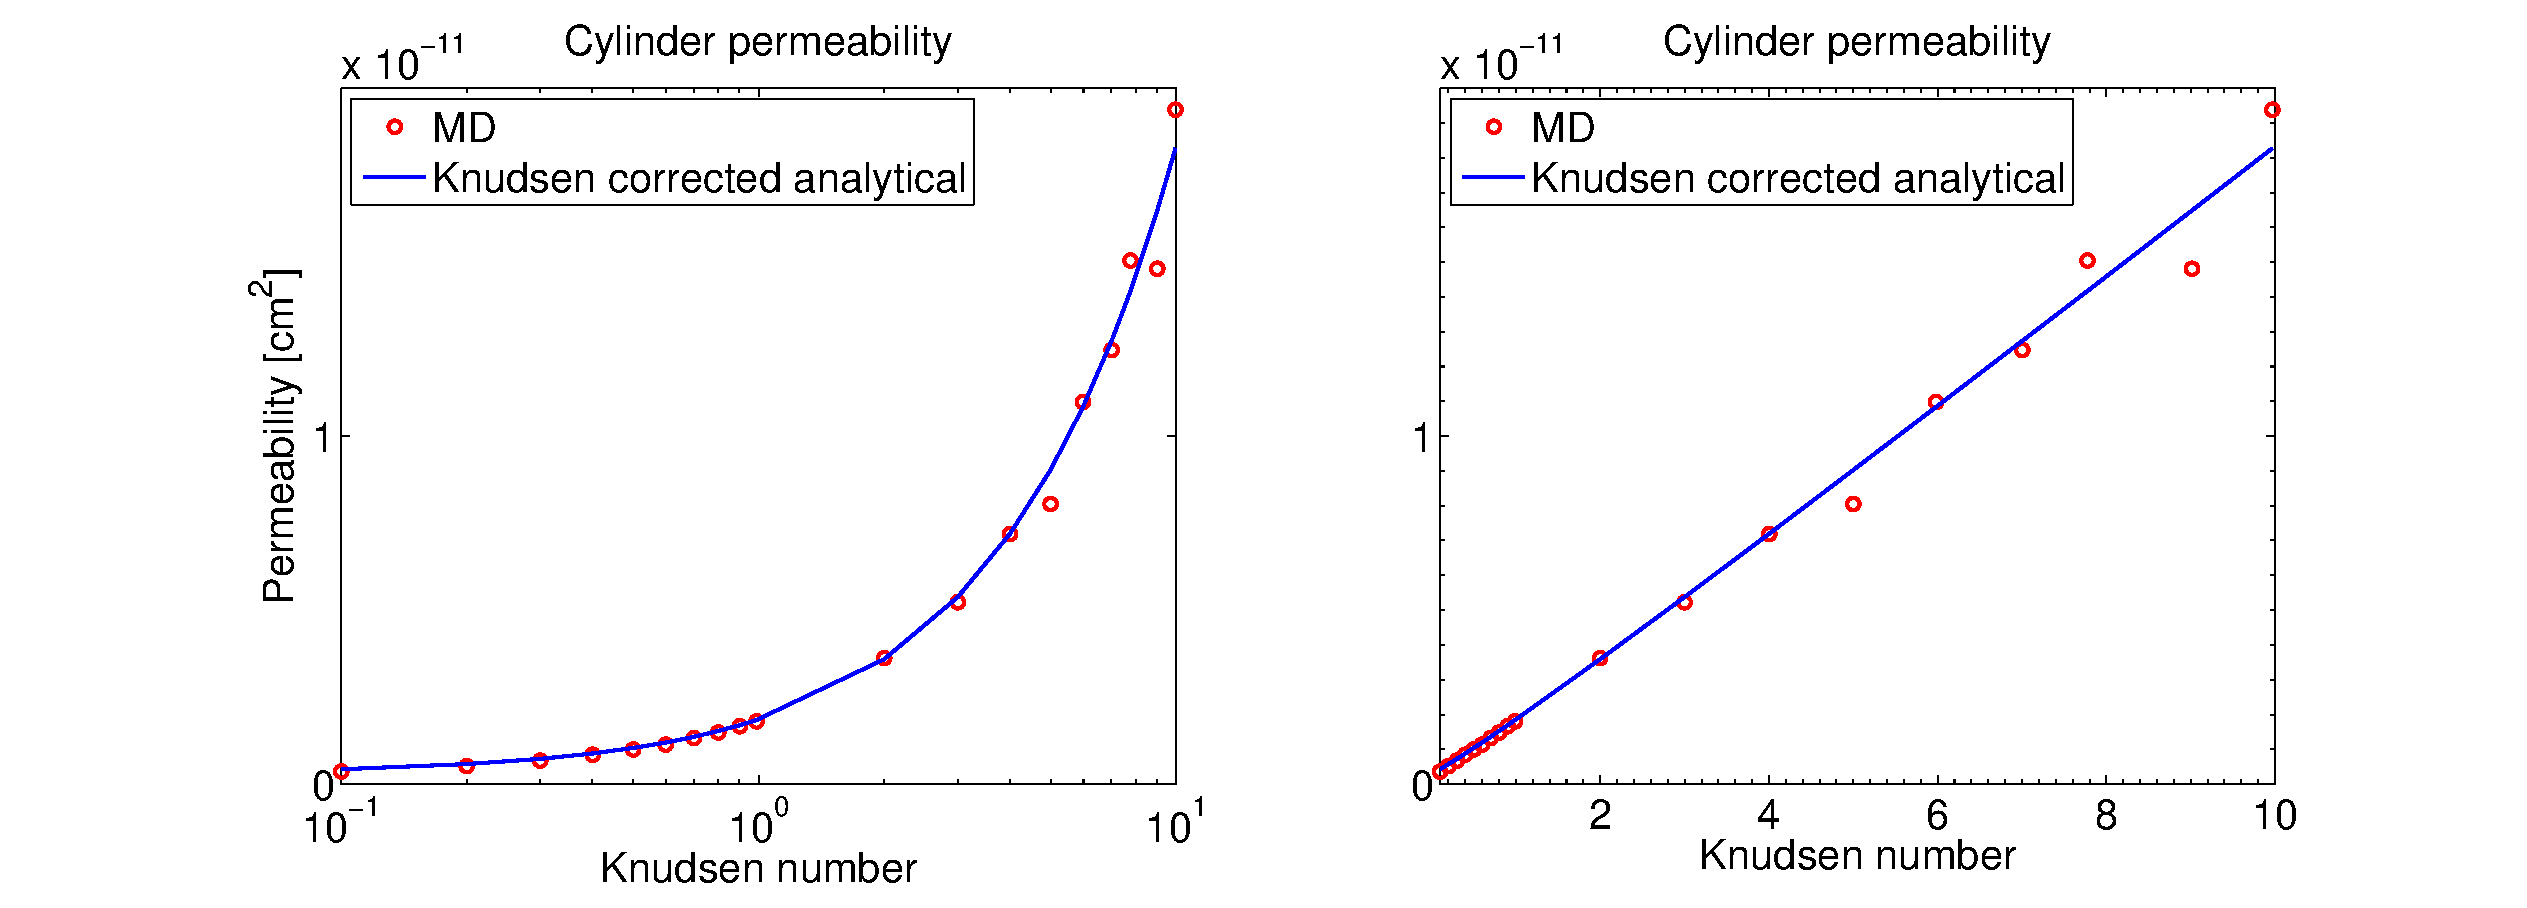
\includegraphics[width=1.0\textwidth, trim=0cm 0cm 0cm 0cm, clip]{MD/figures/permeability_cylinder.eps}
\end{center}
\caption{Permeabilities for Knudsen numbers in the range $0.1$ to $10.0$ in a cylinder with radius $r=$\unit{151}{\angstrom}. The left figure has a logarithmic $x-$axis to emphasize the good prediction in the lower Knudsen range. The right figure shows that the MD code produces results according to the Knudsen corrected permeability for a cylinder in equation \eqref{eq:cylinder_knudsen_corrected} in the entire range. The increased statistical noise is explained by that for large Knudsen numbers, the number of gas atoms is low.}
\label{fig:md_permeability}
\end{figure}
  \end{chapter}  
\end{part}

\begin{part}{Visualization}
  With our newly acquired knowledge about OpenGL and learned how we can use the API to render objects on the screen, we have everything we need to develop our own visualization tools that can handle datasets from both MD and DSMC. As we now should be well aware of, the state of a system with $N$ particles is described by the $3N$ particle positions and the $3N$ velocity components. If we save this information every timestep of a simulation, we can use it to render a time series, an animation of the trajectories of all the particles. We will render the particles as spheres, but areg oing to cheat a bit. An actual sphere rendered in OpenGL would need to be composed of many triangles forming the spherical shape. To be able to render a smooth sphere, we would need more than 100 triangles \textit{per sphere} as we will see in section \ref{sec:vis_billboards}. We will apply a trick used in computer games for years. Instead of rendering spheres, we use something called \textit{billboards}, which is a rectangle with an \textit{image} (a texture) of a sphere, always pointing towards the camera. In section \ref{sec:vis_billboards}, we explain how we effectively can create and render billboards with the goemetry shader on the GPU. If the particle system has periodic symmetry (both MD and DSMC use periodic boundary conditions), we can also use the geometry shader to render copies of the system, making the illusion that the system is larger than it really is.\\
When we visualize a dataset from a DSMC simulation, we should, in addition to the particle positions, render the surface geometry (which, as we remember from section \ref{sec:dsmc_complex_geometries}, is a voxelized scalar field). We will then be able to see the surface the particles collide with which will make it easier to understand their behavior. In section \ref{sec:marching_cubes}, we discuss the so-called \textit{marching cubes} algorithm, which allows us to create a set of renderable triangles from the isosurface of a scalar field (the points where the scalar field values intersect some value).\\
We conclude the chapter by explaining how such a program was extended to render 3D images on an Oculus Rift\footnote{The Oculus Rift is a virtual reality headset displaying a stereoscopic rendering giving realistic 3D effects. The Rift has head tracking, allowing the user to tilt and rotate the head so he/she can look around in the virtual world.} in section \ref{sec:oculus_rift}. The same rendering technique was used to visualize the particles in 3D on a 3D TV.
  \begin{chapter}{OpenGL}
    \section{What is OpenGL?}
\label{sec:opengl}
OpenGL (Open Graphics Library) is an open source graphics library providing an application programming interface (API) to communicate with a graphics processing unit (GPU) in order to get hardware-accelerated \textit{rendering}. Rendering is the process of generating an image from \textit{models} in an \textit{environment}. These models contain information about the geometry and associated textures. A model is typically represented by a set of points, triangles or some other set of \textit{primitives}. Before discussing the model, we should explain what a primitive is.
\subsection{Primitive}
In OpenGL, the primitive decides how to interpret a set of vertices. The same set of vertices may be interpreted, hence rendered, very different on the screen. Three points can be used to draw three single points, a triangle or a part of a rectangle among other different geometries. To illustrate this idea, in figure \ref{fig:opengl_primitives}, the four vertices $\{(0,0), (0,1), (1,1), (1,0)\}$ have been rendered with the primitives \textit{GL\_POINTS}, \textit{GL\_LINES}, \textit{GL\_TRIANGLES}, \textit{GL\_QUADS} and \textit{GL\_TRIANGLE\_STRIP}. The rendered objects are of course very different depending on the primitive. 
\begin{figure}[h]
\begin{center}
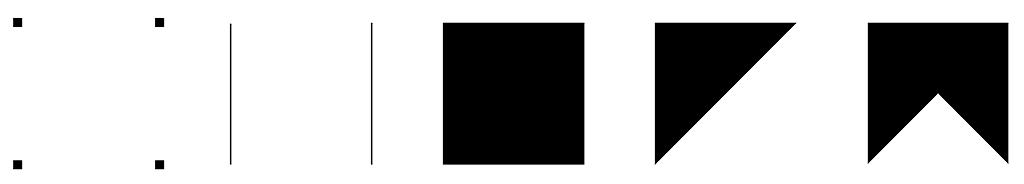
\includegraphics[width=\textwidth, trim=0cm 0cm 0cm 0cm, clip]{opengl/figures/primitives.png}
\end{center}
\caption{The vertices $\{(0,0), (0,1), (1,1), (1,0)\}$ have been rendered as the primitives (from left) \textit{GL\_POINTS}, \textit{GL\_LINES}, \textit{GL\_TRIANGLES}, \textit{GL\_QUADS} and \textit{GL\_TRIANGLE\_STRIP}. We see that the final rendered geometrical objects are quite different for the different primitives.}
\label{fig:opengl_primitives}
\end{figure}
When using for example the \textit{GL\_TRIANGLES}, OpenGL interprets groups of three vertices as one triangle. In the case of \textit{GL\_QUADS}, it will of course use groups of four vertices to define the renderable object. All of the primitives (except the \textit{GL\_POINTS}) form one or more two dimensional surfaces that are colored from either the interpolated values between the vertices or from a texture map which we now will explain.
\subsection{Color interpolation}
\label{sec:opengl_color_interpolation}
When creating a primitive consisting of $N$ vertices we can color each vertex $\vec r_i$ with an RGBA vector
\begin{align}
	\vec c_i = (r_i, g_i, b_i, \alpha_i)
\end{align}
where the components are the red, green, blue and alpha values for vertex $i$. The first three components defines the color whereas the last component is the transparency. In between the $N$ vertices, there are a lot of points that do not have a defined color value. OpenGL assigns colors to these inner points by \textit{linearly interpolating} the color values of the vertices. Any point $\vec p$ in a triangle defined by the three vertices $\vec p_a, \vec p_b$ and $\vec p_c$ can be uniquely specified by using \textit{barycentric coordinates} which is a set of three numbers $(a,b,c)$ in the range $[0,1]$, normalized so that $a+b+c=1$. \todo{cite the opengl specification} Once we have these coordinates, the point $\vec p$ in the global coordinate system (in which the vertices $\vec p_i$ are defined) is found as
\begin{align}
	\vec p = a\vec p_a + b\vec p_b + c\vec p_c.
\end{align}
The barycentric coordinates are found through
\begin{align}
	a = \frac{A(\vec p, \vec p_b, \vec p_c)}{A(\vec p_a, \vec p_b, \vec p_c)}, \qquad b = \frac{A(\vec p, \vec p_a, \vec p_c)}{A(\vec p_a, \vec p_b, \vec p_c)}, \qquad c = \frac{A(\vec p, \vec p_a, \vec p_b)}{A(\vec p_a, \vec p_b, \vec p_c)}.
\end{align}
We then use the barycentric coordinates as the weights in the linear interpolation so that the color at a point $\vec p$ is given as
\begin{align}
	\vec c(\vec p) = a\vec c_a + b\vec c_b + c\vec c_c,
\end{align}
where $\vec c(\vec p_i)$ is the color we gave the vertex at $\vec p_i$. In figure \ref{fig:opengl_color_interpolation} we see how the colors are interpolated from the three values at the triangle vertices.
\begin{figure}[h]
\begin{center}
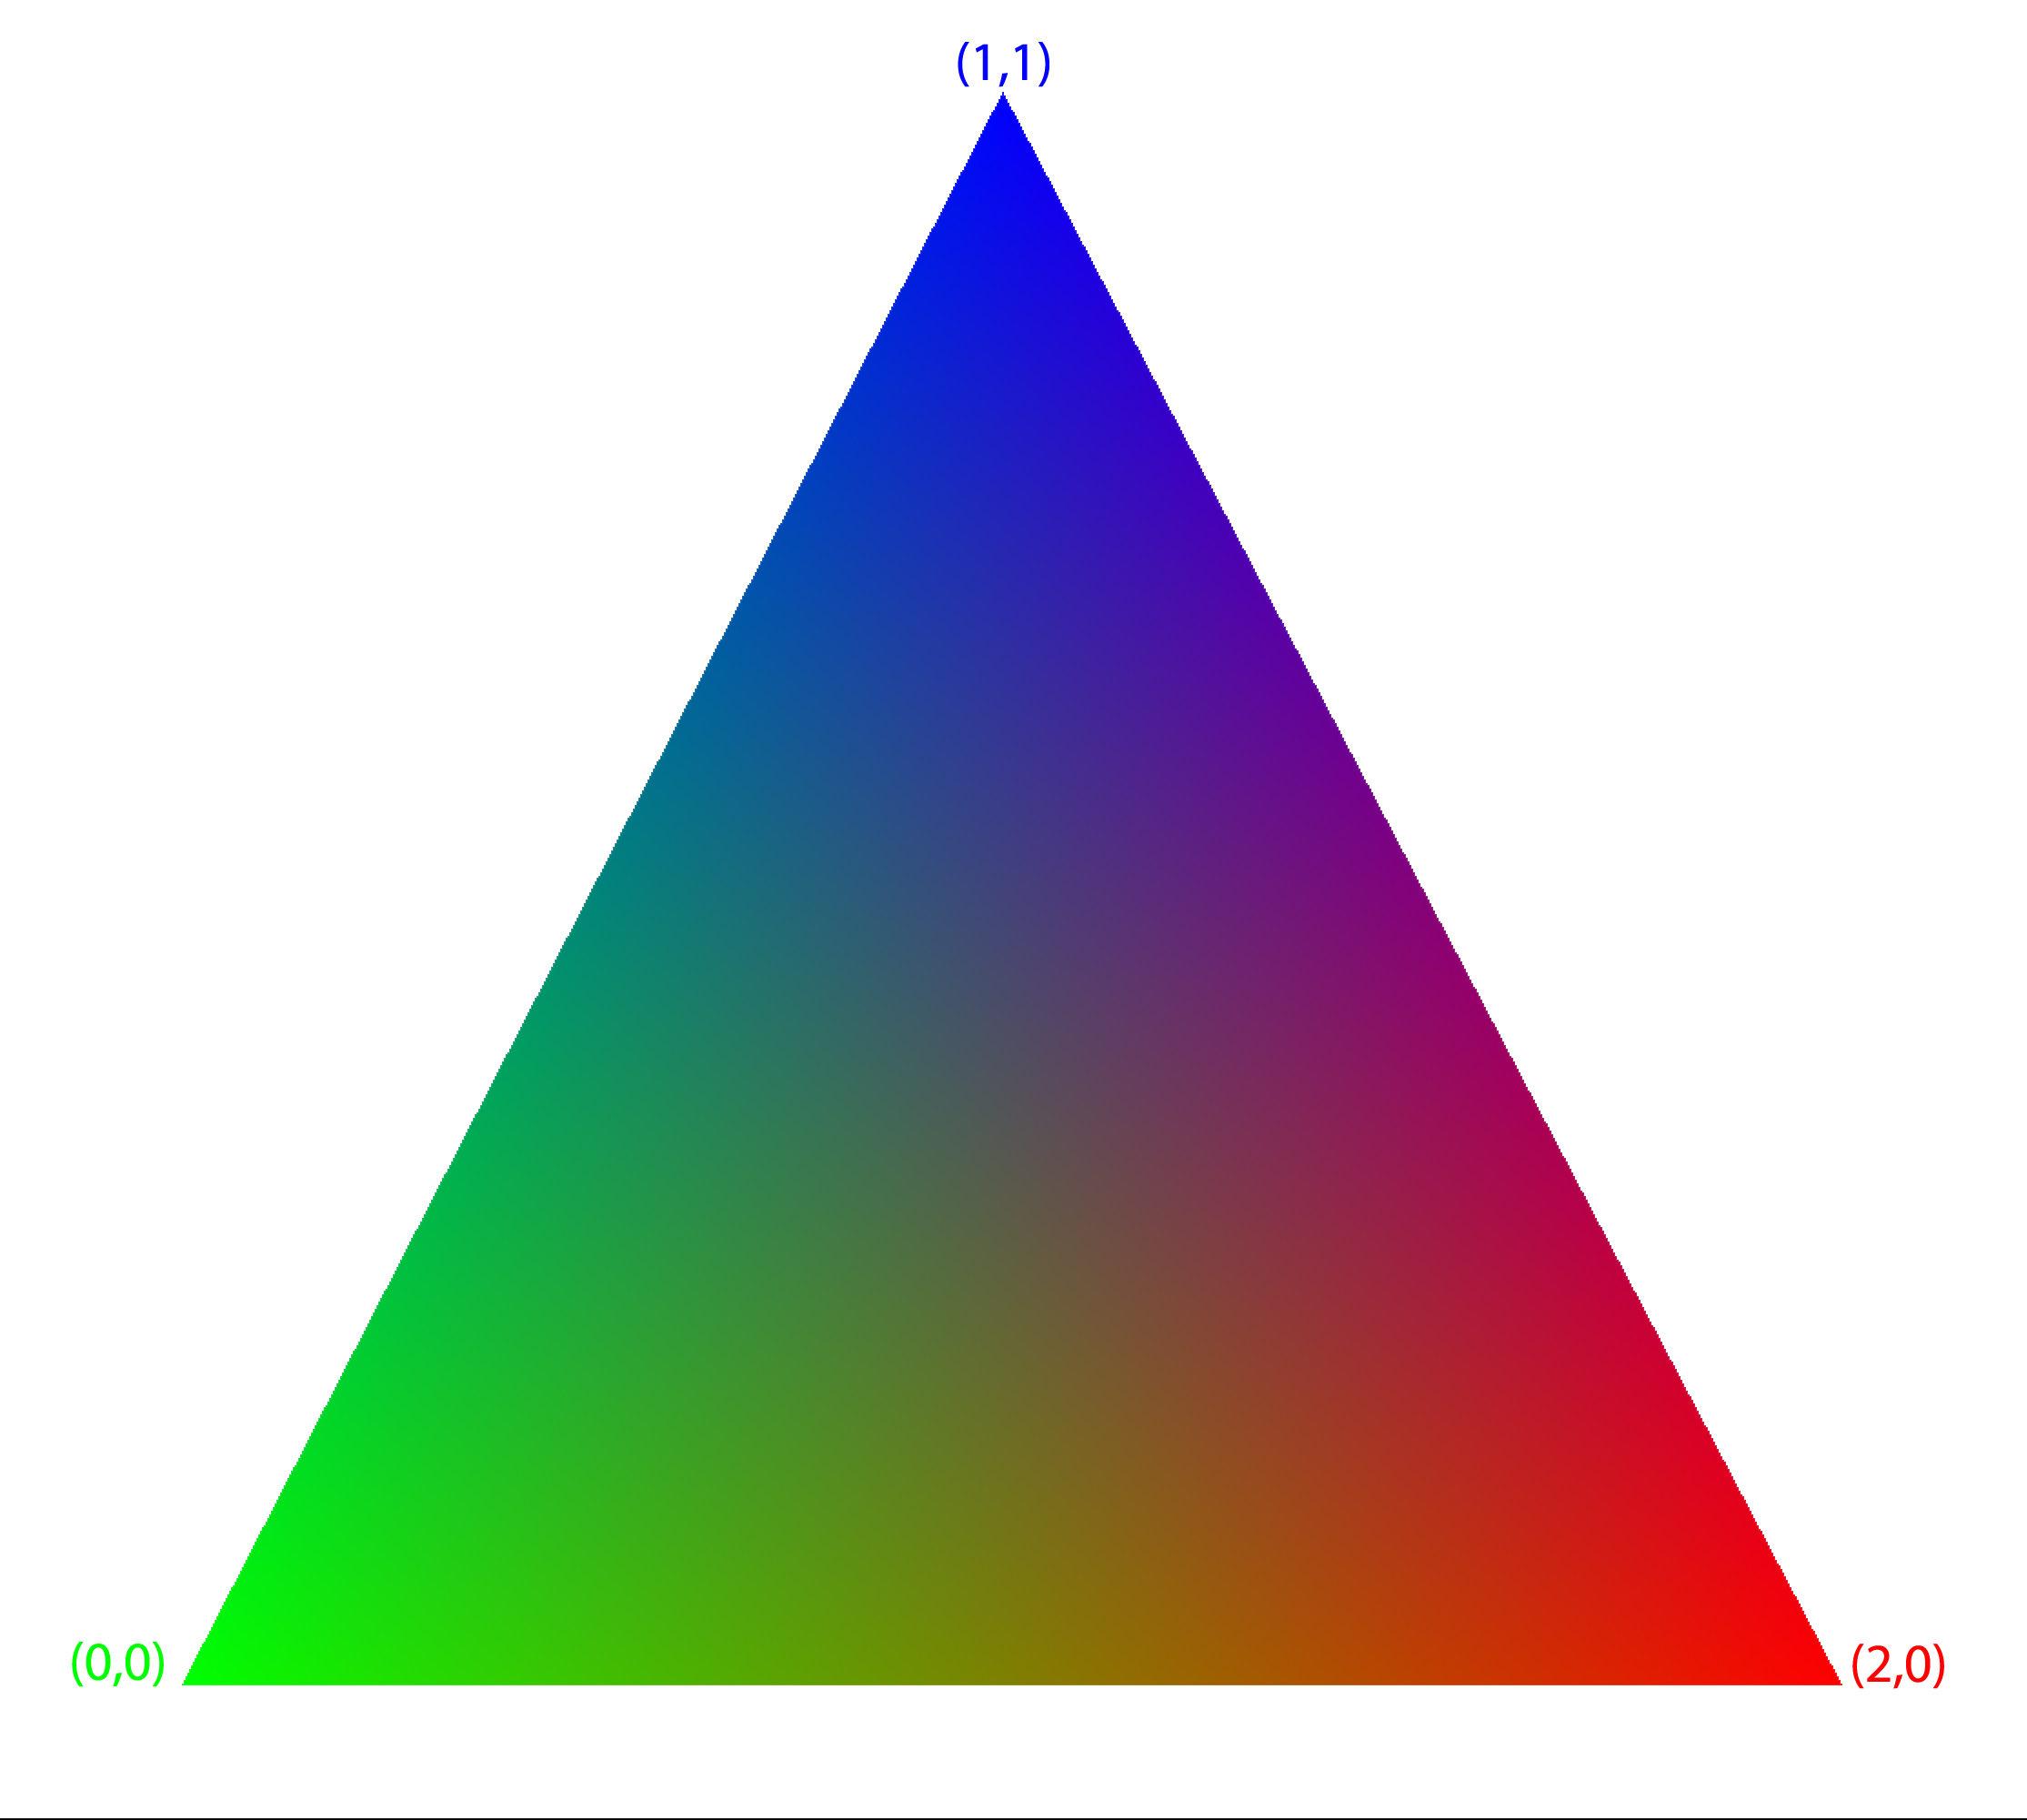
\includegraphics[width=\textwidth, trim=0cm 0cm 0cm 0cm, clip]{opengl/figures/color_interpolation.png}
\end{center}
\caption{The three vertices $\{(0,0), (1,1), (2,0)\}$ colored green, blue and red, forms a triangle where the inner points of the triangle is colored by the interpolation between the three vertices.}
\label{fig:opengl_color_interpolation}
\end{figure}
\subsection{Textures}
\label{sec:opengl_texture_interpolation}
Instead of using the colors specified per vertex, we can upload a texture (for example an image) to the graphics card so that the GPU can use that as the source of the color (this can be combined with the color values as we will see soon). The texture consists of $m\times n$ pixels where each pixel has a color $\vec c_t$. Each vertex $i$ of the triangle is assigned a \textit{local texture coordinate} 
\begin{align}
	\vec t_i = (t_x, t_y),
\end{align}
where $t_x, t_y \in [0,1]$. This gives the mapping to the \textit{global texture coordinates} (the actual pixel coordinates) $\vec t^* = (t_x^*, t_y^*)$ where 
\begin{align}
	\nonumber
	t_x^* &= m\cdot t_x\\
	t_y^* &= n\cdot t_y,
\end{align}
where we have added the asterisk on the global coordinates since we will mostly use the local ones. Since each pixel $\vec t$ (remember these are the local coordinates) in the texture has a color value $\vec c_t(\vec t)$, we can find the color $\vec c(\vec p)$ of a point $\vec p$ within the triangle by interpolating the local texture coordinates as we interpolated the colors. Remember that the point $\vec p$ has barycentric coordinates $(a,b,c)$, so the local texture coordinates $\vec t$ are found by
\begin{align}
	\vec t(\vec p) =  a\vec t_a + b\vec t_b + c\vec t_c,
\end{align}
where $\vec t_i$ is the local texture coordinate assigned to vertex $i$. The color of this point $\vec p$ is then simply
\begin{align}
	\vec c(\vec p) = \vec c_t[\vec t(\vec p)].
\end{align}
In figure \ref{fig:opengl_texture_interpolation} we have illustrated how the texture interpolation works. In the left figure, the texture is mapped with  texture coordinates corresponding to the coordinates of the triangle vertices. In the figure to the right we have a skewed mapping making the image look skewed.
\begin{figure}[h]
\begin{center}
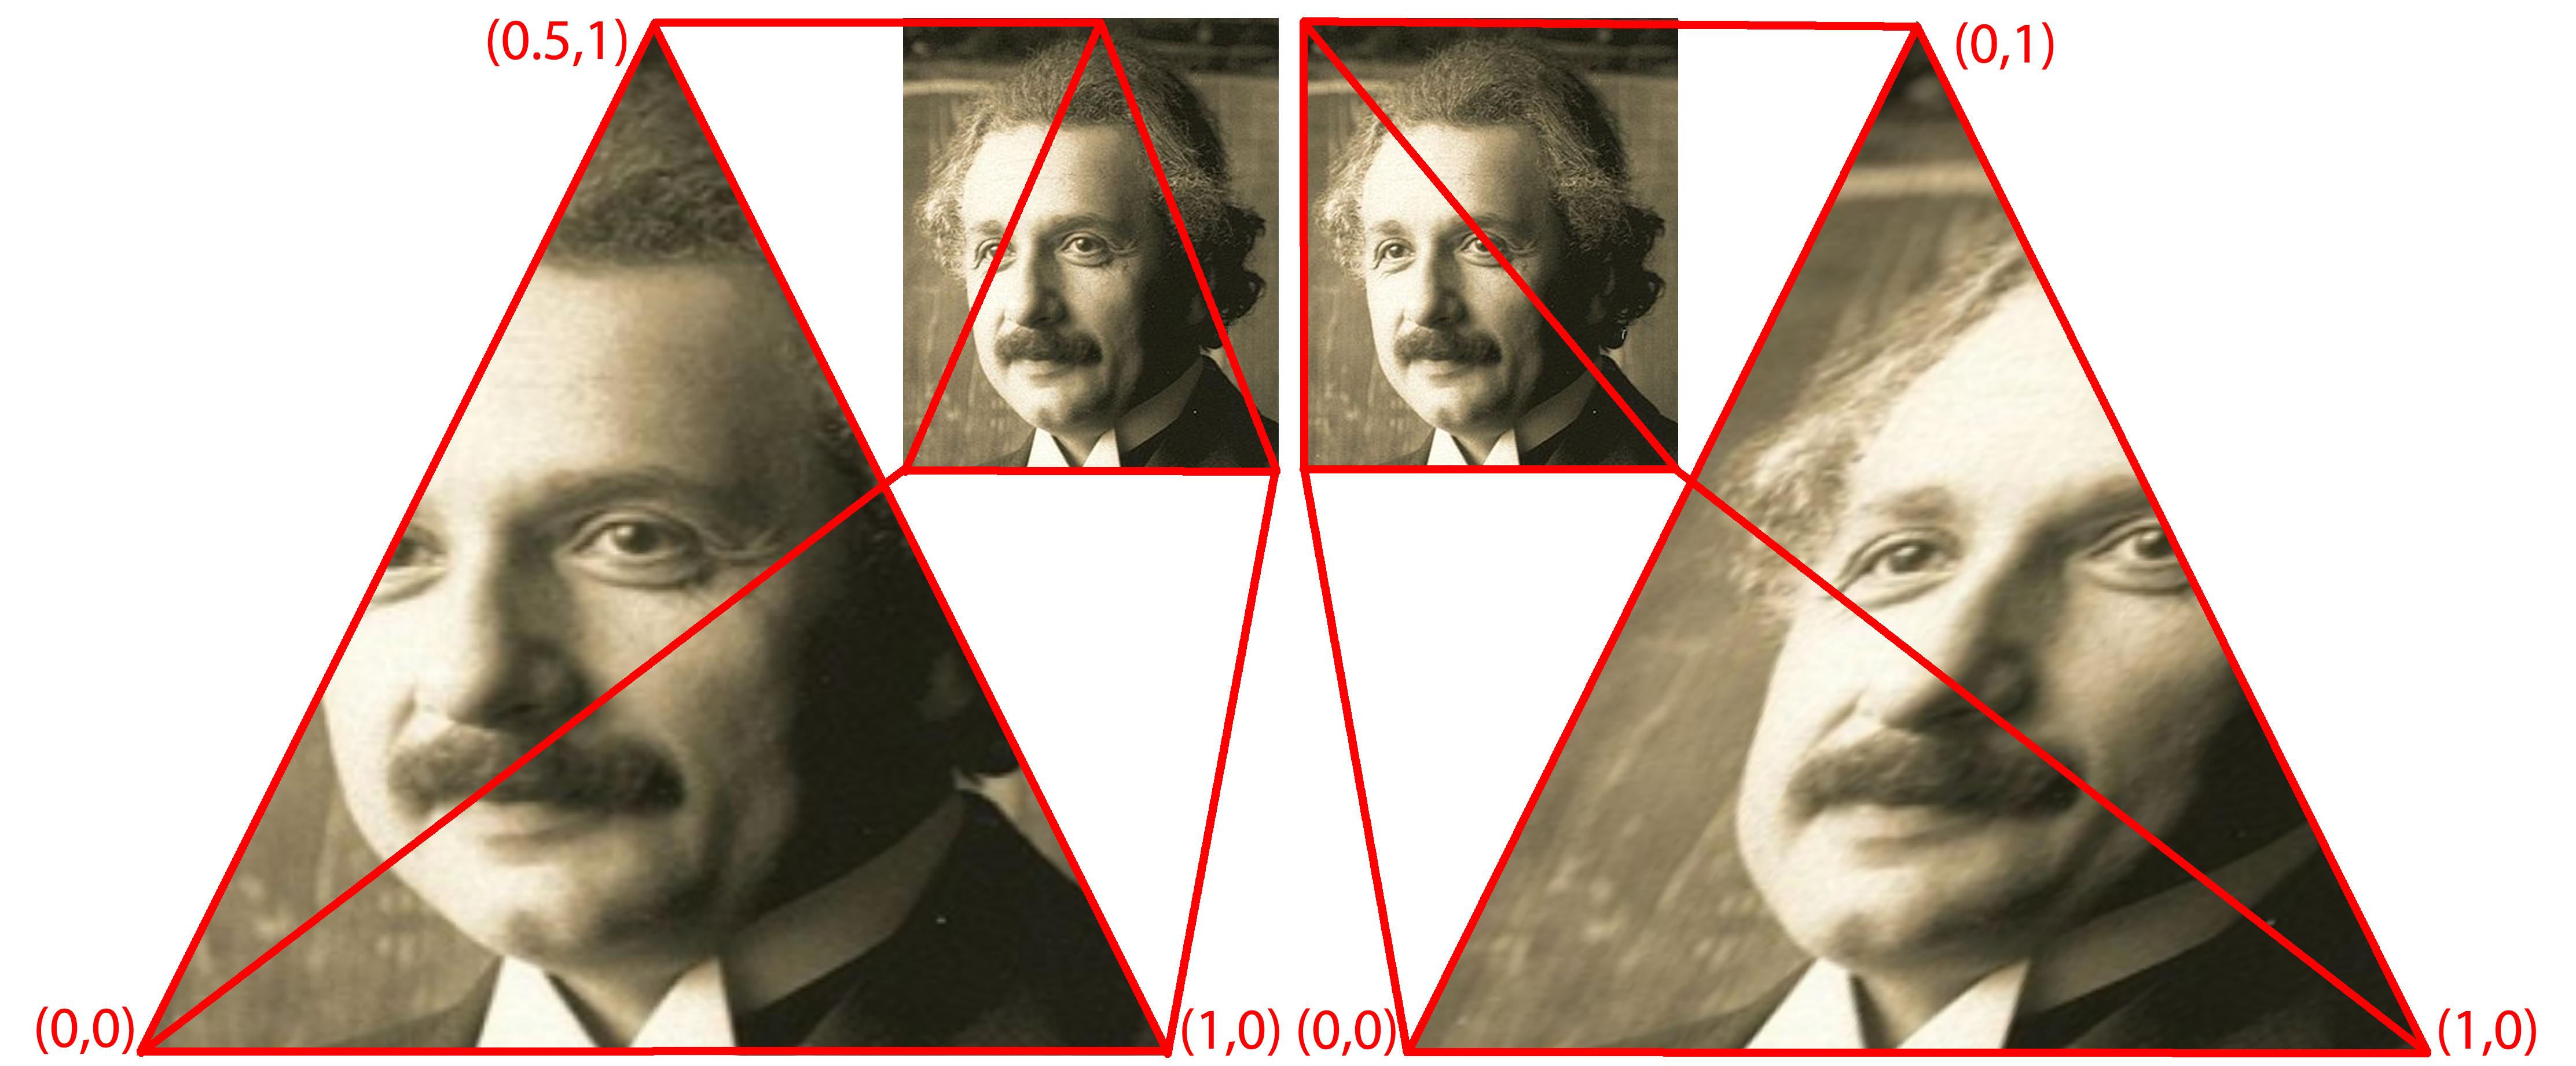
\includegraphics[width=\textwidth, trim=0cm 0cm 0cm 0cm, clip]{opengl/figures/texture_interpolation.png}
\end{center}
\caption{Showing how texture interpolation works. Left: the three vertices $\{(0,0), (1,1), (2,0)\}$ are assigned the local texture coordinates $\{(0,0), (0.5,1), (1,0)\}$ where we see how the texture are transformed onto the triangle . Right: the three vertices $\{(0,0), (1,1), (2,0)\}$ are assigned the local texture coordinates $\{(0,0), (0,1), (1,0)\}$ where we see that the texture on the triangle is skewed because of the transformation. Note that the coordinates in the figure at the vertices are the texture coordinates, not the coordinates of the vertices.}
\label{fig:opengl_texture_interpolation}
\end{figure}
We can of course combine both these methods (colors and textures) by applying both a texture coordinate \textit{and} a color value to each vertex. OpenGL will then render an image where the rendered color $\vec C$ becomes
\begin{align}
	\label{eq:opengl_combining_colors_textures}
	\vec C(\vec p) = \vec c_t[\vec t(\vec p)] \odot \vec c(\vec p),
\end{align}
where $\odot$ is the element-wise multiplication operator defined as
\begin{align}
	(\vec a \odot \vec b)_i = a_i\cdot b_i,
\end{align}
where $\vec a,\vec b \in \mathbb{R}^N$ and $d_i$ is the $i$'th component of some vector $\vec d$. In figure \ref{fig:color_and_texture} we have combined both the color and the texture giving a triangle with the same image of Albert Einstein colored in the same way as the triangle in figure \ref{fig:opengl_color_interpolation}.
\begin{figure}[h]
\begin{center}
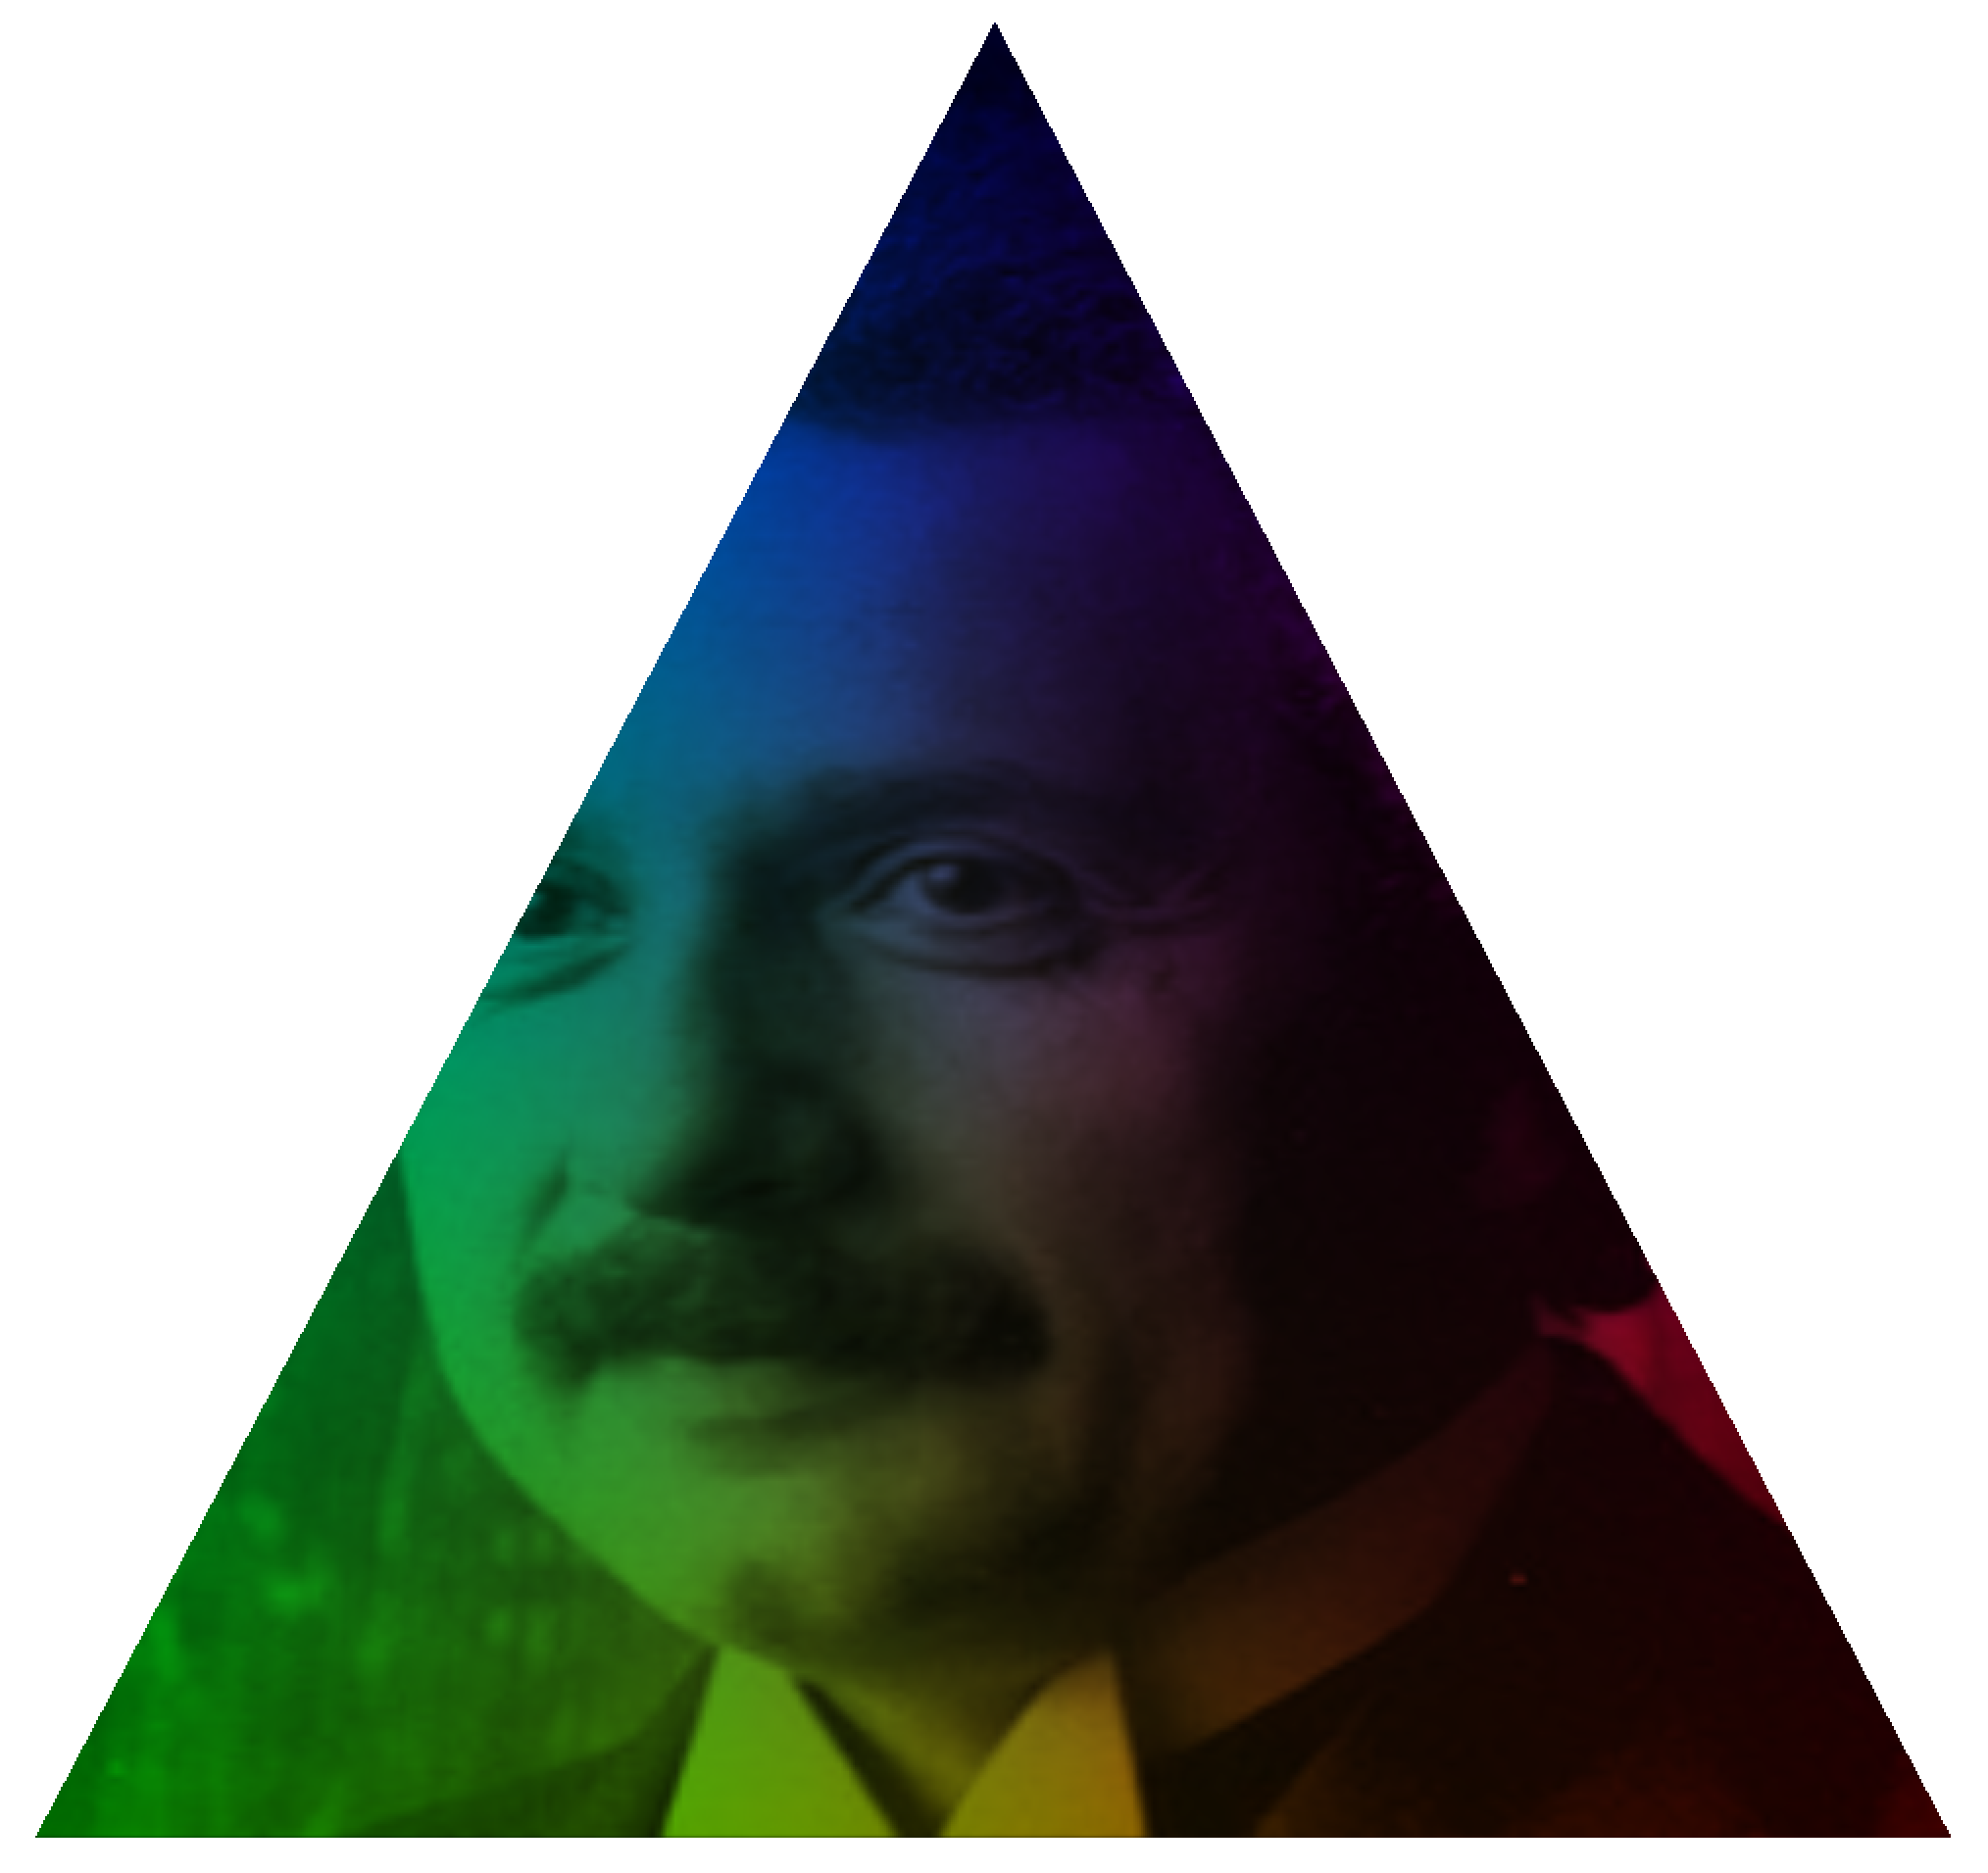
\includegraphics[width=\textwidth, trim=0cm 0cm 0cm 0cm, clip]{opengl/figures/color_and_texture.png}
\end{center}
\caption{We can combine both colors and textures to color points within a triangle according to equation \eqref{eq:opengl_combining_colors_textures}. Here we have used the same colors as in figure \ref{fig:opengl_color_interpolation} and the texture of Albert Einstein in figure \ref{fig:opengl_texture_interpolation}.}
\label{fig:color_and_texture}
\end{figure}
\subsection{Model}
\label{sec:opengl_model}
A model of an object contains all the information fully defining how a geometric object looks like without any effects from the environment such as light or distortions from a water surface. The model is fully described by a set $\mathcal{M}$ containing primitive objects $\mathcal{P}$, each having 
\begin{itemize}
	\item a vertex array,
	\item the primitive type,
	\item a color array,
	\item a texture id,
	\item a local texture coordinate array, and
	\item a normal vector array.
\end{itemize}
We have discussed the array of vertices, the primitive, the color and texture coordinate arrays (remember, one color and/or one texture coordinate per vertex). We also need the id (which is just an int variable) allowing us to tell the GPU which texture it should apply to this primitive object. In addition, we can assign a \textit{normal vector} to each vertex which can be used to create realistic lighting and other effects. It's time for an example of a model.\\
Say we want a model of a die. A die is a cube with six faces. The model $\mathcal M$ would then contain six primitive objects $\mathcal P_i$, each having an array of four vertices. The primitive type would be \textit{GL\_QUADS} where the color of course could be your favorite. We need to upload six textures (one face has one dot, another face has two dots etc) which gives us six different texture id's. The local texture coordinate array is simply the four corners of the unit square whereas the normal vectors should point outwards from the cube. In figure \ref{fig:opengl_die} we haved used this technique to draw a red die.
\begin{figure}[h]
\begin{center}
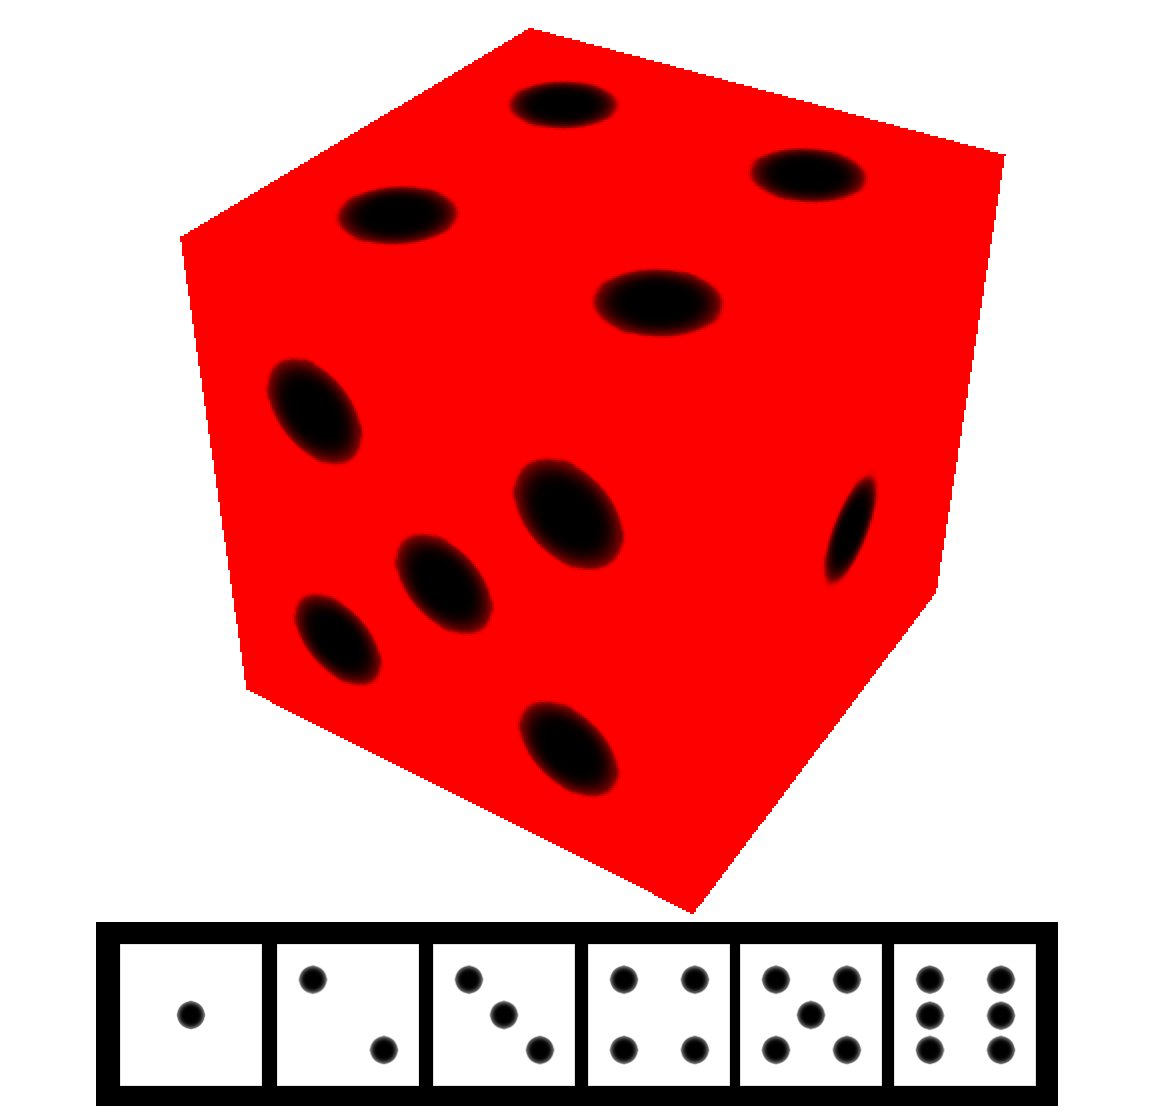
\includegraphics[width=\textwidth, trim=0cm 0cm 0cm 0cm, clip]{opengl/figures/die.png}
\end{center}
\caption{Drawing a die using the technique described in subsection \ref{sec:opengl_model}. The color was chosen to be red whereas each of the six faces were assigned one of the textures in the black box.}
\label{fig:opengl_die}
\end{figure}
    \input{opengl/functions}
    \section{Coordinate transformations}
\label{sec:opengl_coordinate_transformations}
\subsection{Model space}
\subsection{View space}
\subsection{Projection space}
    \input{opengl/textures}
    \input{opengl/shaders}
    \section{Vertex Buffer Objects}
\label{sec:opengl_vbo}
A Vertex Buffer Object (VBO) is a feature in OpenGL that allows the user to upload an array of vertices to the graphics card which can be used for fast rendering. This could for example be a set of positions, colors or normal vectors. Once this data is uploaded to the GPU, we can render the model described by the VBO in very few function calls. First, we ask the GPU to give us a buffer identifier (which is just an int) that we will use when we work with the VBO (uploading new data or using the data). Then we tell the GPU to allocate enough memory to store our vertices before we copy the data from the main memory to the graphics card.
  \end{chapter}

  \begin{chapter}{Results}
    \section{Marching Cubes}

  \end{chapter}
\end{part}

\begin{part}{Conclusion}
  
\end{part}
%---------------------------------------------------------------------------------------
% Appendices
%---------------------------------------------------------------------------------------
\begin{appendices}

\end{appendices}

%---------------------------------------------------------------------------------------
% Bibliography
%---------------------------------------------------------------------------------------
\printbibliography
\end{document}